\documentclass[11pt,a4paper,oneside]{report}
\usepackage[T1]{fontenc}
\usepackage[utf8]{inputenc}
\usepackage{lmodern,microtype}
\usepackage[a4paper,left=24mm,right=24mm,top=23mm,bottom=25mm,headheight=14pt]{geometry}
\usepackage{amsmath,amssymb,amsthm,mathtools,bm}
\usepackage{booktabs,longtable,array,enumitem,xcolor,needspace}
\usepackage{graphicx}
\usepackage[round,authoryear]{natbib}
\usepackage{titlesec,fancyhdr}
\usepackage{xurl}
\usepackage{hyperref}
\definecolor{inkblue}{HTML}{234F67}
\definecolor{inkgrey}{HTML}{4B5459}
\hypersetup{colorlinks=true,linkcolor=inkblue,citecolor=inkblue,urlcolor=inkblue,
  pdftitle={Derivations of additive channels: mathematical foundations and biological interpretation},
  pdfauthor={Daniel Ortiz-Barrientos and Mark Cooper},
  pdfsubject={Detailed mathematical derivations and their biological interpretation}}
\urlstyle{same}
\titleformat{\chapter}[display]{\normalfont\Large\bfseries\color{inkblue}\raggedright\hyphenpenalty=10000}
 {\large\chaptertitlename\ \thechapter}{6pt}{\LARGE}
\titlespacing*{\chapter}{0pt}{-6pt}{18pt}
\titleformat{\section}{\normalfont\large\bfseries\color{inkblue}}{\thesection}{0.7em}{}
\titleformat{\subsection}{\normalfont\normalsize\bfseries}{\thesubsection}{0.7em}{}
\setlength{\parindent}{0pt}
\setlength{\parskip}{5pt plus 1pt minus 1pt}
\setlength{\emergencystretch}{2em}
\setlist{topsep=4pt,itemsep=3pt,parsep=1pt,leftmargin=*}
\allowdisplaybreaks[1]
\numberwithin{equation}{chapter}
\pagestyle{fancy}
\fancyhf{}
\fancyhead[L]{\small\color{inkgrey}Additive channels: derivation companion}
\fancyhead[R]{\small\color{inkgrey}\thepage}
\renewcommand{\headrulewidth}{0.3pt}
\fancypagestyle{plain}{\fancyhf{}\fancyfoot[C]{\small\thepage}\renewcommand{\headrulewidth}{0pt}}
\newcommand{\vect}[1]{\boldsymbol{#1}}
\newcommand{\mat}[1]{\mathbf{#1}}
\newcommand{\bGamma}{\boldsymbol{\Gamma}}
\newcommand{\bgamma}{\boldsymbol{\gamma}}
\newcommand{\E}{\mathbb E}
\newcommand{\Var}{\operatorname{Var}}
\newcommand{\Cov}{\operatorname{Cov}}
\newcommand{\Corr}{\operatorname{Corr}}
\newcommand{\tr}{\operatorname{tr}}
\newcommand{\Ag}{\mathcal A_g}
\newcommand{\Vlin}{V_{\mathrm{lin}}}
\newcommand{\Vquad}{V_{\mathrm{quad}}}
\newcommand{\Gsel}{\mat G_{\mathrm{sel}}}
\newcommand{\norm}[1]{\left\lVert #1\right\rVert}
\newcommand{\R}{\mathbb R}
\newcommand{\given}{\mid}
\newtheorem{theorem}{Theorem}[chapter]
\newtheorem{proposition}[theorem]{Proposition}
\newtheorem{lemma}[theorem]{Lemma}
\newtheorem{corollary}[theorem]{Corollary}
\theoremstyle{definition}
\newtheorem{definition}[theorem]{Definition}
\newtheorem{example}[theorem]{Example}
\theoremstyle{remark}
\newtheorem{remark}[theorem]{Remark}
\newcommand{\codepath}[1]{{\urlstyle{tt}\nolinkurl{#1}}}
\newcommand{\repofile}[2]{\href{https://github.com/dortizbarrientos/additive_channels/blob/main/#1}{#2}}
\begin{document}
\begin{titlepage}
\vspace*{15mm}
{\large\color{inkblue}ADDITIVE CHANNELS\par}
\vspace{9mm}
{\Huge\bfseries Derivations of\par additive channels\par}
\vspace{7mm}
{\Large Mathematical foundations and\par biological interpretation\par}
\vspace{14mm}
{\large Daniel Ortiz-Barrientos and Mark Cooper\par}
\vspace{6mm}
13 November 2026\par
\vfill
\begin{minipage}{0.93\textwidth}
A derivation companion for readers who want to follow each mathematical result from its assumptions through its algebra to its biological meaning. The result map connects the proofs and worked calculations to the numerical reproduction code, figures, supplementary examples and interactive resources.
\end{minipage}\par
\vspace{10mm}
\href{https://github.com/dortizbarrientos/additive_channels}{github.com/dortizbarrientos/additive\_channels}
\end{titlepage}
\pagenumbering{roman}
\chapter*{How to use this companion}
\addcontentsline{toc}{chapter}{How to use this companion}
\label{reading:map}

The linear share measures the fraction of variance supplied by the linear term of a stated quadratic approximation to log expected reproductive output. We call a population--fitness relationship with a large linear share an additive channel. To interpret that description, we need to know what has been averaged, which population supplies the frequency weights, and which assumptions permit a linear and a curved contribution to be separated. To predict selection, we must then change the weights to account for reproductive output. To predict a later generation, we must additionally specify inheritance.

This companion follows that sequence. It develops the calculations behind \emph{Additive channels in curved fitness landscapes}, its mathematical appendices, mathematics guide, estimation example and visual tutorials. It expands the intermediate steps that a shorter scientific account can leave implicit: Gaussian moment contractions, population regression normal equations, matrix factorisations, normalising integrals, covariance order, fixed-point arguments and integration over uncertain breeding values. It also states the biological assumptions that make each calculation relevant.

The accompanying repository contains numerical reproductions, data generated under the stated models, and teaching resources. The proofs here are analytical. A numerical check can confirm an implementation or expose an error in a stated case; agreement in finitely many examples cannot prove a general identity. Conversely, the reported fitted estimates, simulation discrepancies and bootstrap endpoints are outputs of specified algorithms and random seeds. Their mathematical definitions and procedures can be derived, but their particular values must be reproduced computationally. Chapter~\ref{worked:chapter} treats that distinction explicitly.

\section*{Three routes through the document}
Read Chapters~\ref{conditioning:chapter}--\ref{inheritance:chapter} in order to follow the theoretical argument from expected reproduction to an inheritance model. Continue with Chapters~\ref{estimation:chapter} and~\ref{conversion:chapter} to connect those quantities to observations and phenotype-space regressions. If you need one particular result, use the linked result map in Appendix~\ref{coverage:chapter}; it covers every entry in the repository's 53-record result catalogue. The equation map in Section~\ref{coverage:equations} also connects all 106 source-qualified equation labels to their detailed derivations or definitions.

Each substantial derivation identifies the mathematical tools it uses and explains the biological interpretation afterwards. The prerequisites are developed where they first become necessary. Familiarity with derivatives, finite sums, vectors and matrices will help; familiarity with Gaussian quadratic forms or matrix order is not assumed. The distinction between a selected-parent distribution and an offspring distribution is maintained throughout.

\begin{longtable}{@{}>{\raggedright\arraybackslash}p{0.24\textwidth}>{\raggedright\arraybackslash}p{0.41\textwidth}>{\raggedright\arraybackslash}p{0.27\textwidth}@{}}
\toprule
Mathematical concept & Why it is needed & Start here \\
\midrule\endhead
Conditional expectation & Average reproductive output without confusing it with individual observations; obtain parental weights. & Chapter~\ref{conditioning:chapter} \\
Taylor expansion and moments & Specify the quadratic target and calculate its population variance. & Chapter~\ref{gaussian:chapter} \\
Least-squares projection & Identify the fitted intercept, slopes and explained variance under population frequencies. & Chapter~\ref{gaussian:chapter} \\
Eigenvalues and coordinate changes & Separate changes in trait units from changes in biological variation. & Chapter~\ref{geometry:chapter} \\
Normalisation and quadratic forms & Calculate selected-parent moments and determine when the reproductive weights are integrable. & Chapter~\ref{selection:chapter} \\
Matrix order and fixed points & Determine which covariances can persist under the specified inheritance closure. & Chapter~\ref{inheritance:chapter} \\
Likelihood and latent integration & Estimate the fitness relationship while accounting for uncertainty in breeding values. & Chapter~\ref{estimation:chapter} \\
Conditional Gaussian moments & Convert compatible phenotype-regression moments into breeding-value-space quantities. & Chapter~\ref{conversion:chapter} \\
\bottomrule
\end{longtable}

\section*{Notation and units}
Vectors are columns. Bold capital letters denote matrices unless they identify a random vector. The transpose is $\mathsf T$. A covariance matrix is symmetric and positive semidefinite. The notation $\mat G\succ0$ adds strict positive definiteness; inverses require it, or an explicit restriction to the subspace with positive variance.

\begin{longtable}{@{}p{0.22\textwidth}p{0.70\textwidth}@{}}
\toprule Symbol & Meaning \\
\midrule\endhead
$\vect A$, $\vect a$ & Random breeding-value vector and a possible value. Breeding values sum population-specific average allelic effects; the inheritance model later makes stronger fixed-effect assumptions. \\
$\bar{\vect A}$, $\vect X$ & Population mean and centred deviation $\vect A-\bar{\vect A}$. \\
$\mat G$ & Breeding-value covariance in the population used to define the fitness description. \\
$W$, $W_A(\vect a)$ & Reproductive output and its conditional mean $\E[W\mid\vect A=\vect a]$. \\
$\ell_A(\vect a)$ & $\log W_A(\vect a)$ where the conditional mean is positive. All logarithms are natural. \\
$\ell_0$, $\vect b$, $\mat H$ & Value, gradient and Hessian of $\ell_A$ at the reference mean. Their units are respectively log output, reciprocal trait units, and reciprocal products of trait units. \\
$\widetilde\ell_A$ & The stated second-order polynomial. It equals the full log conditional mean only under an exact log-quadratic model. \\
$L$, $Q_c$ & Linear and centred quadratic terms of that polynomial. \\
$\Vlin$, $\Vquad$, $\Ag$ & Variances of those terms and the linear fraction $\Vlin/(\Vlin+\Vquad)$ when the denominator is positive. These are quantities on the log expected-output scale. \\
$\bGamma$ & $-\mat H$. Stabilising curvature means $\bGamma\succeq0$. Some selection calculations also allow indefinite curvature if the combined precision is positive definite. \\
$\Gsel$, $\vect\Delta$ & Covariance and mean displacement under reproductive weighting of parents. \\
$\mat B$, $\rho$ & Fixed genic covariance and the specified fraction of the selected covariance's departure from it retained after reproduction. \\
$\mat P$, $\vect\beta$, $\bgamma$ & Phenotype covariance and linear/quadratic coefficients of a compatible raw relative-fitness regression. They are not automatically $\mat G$, $\vect b$ and $\mat H$. \\
\bottomrule
\end{longtable}

The meaning of a subscript is stated where it is introduced. In the estimation chapter, the offspring count and prediction reliability have separate symbols. Environmental variance in a fitness assay and measurement variance in repeated trait observations also require separate biological assumptions, even when both have Gaussian distributions.

\section*{Versions and scope}
The mathematical results correspond to the public code archive at \href{https://github.com/dortizbarrientos/additive_channels/tree/05c75c6ee4335513b217f3026bf6e43ccbd0f62b}{commit \texttt{05c75c6}}. The result catalogue, expanded checks and resource organisation used for this companion are those at \href{https://github.com/dortizbarrientos/additive_channels/tree/c860f6a1373be310a59502e244effe75e0e622be}{commit \texttt{c860f6a}}. The present companion adds explanations and proof steps; it does not change the generating models or their reference numerical results. Its source, result map and build instructions accompany this PDF in the same repository.

The assumptions strengthen at distinct points. Gaussian moments give an exact variance partition for a quadratic polynomial. Exact selected-parent formulas require an integrable exponential quadratic fitness function. The covariance recursion additionally assumes a fixed genic baseline and a specified inheritance closure. Estimation introduces its own observation model. None of these later assumptions follows merely from a large value of $\Ag$.

\tableofcontents
\clearpage
\pagenumbering{arabic}
\chapter{Conditional fitness, reproductive contributions and logarithms}
\label{conditioning:chapter}

An individual's breeding value does not determine its realised reproductive
output. Individuals with the same breeding value can differ in environment,
genetic background and unmeasured traits, and reproduction itself can be
stochastic. We therefore begin with an average over the individuals represented
at each breeding value. This chapter derives what that average supplies, why its
logarithm is taken after averaging, and how environmental variation changes it.
The variance calculations in Chapter~\ref{gaussian:chapter} then describe
variation in this specified quantity.

\section{A conditional mean defines the fitness relationship}

Let \(\vect A\) denote breeding value in a specified population and let \(W\)
denote nonnegative reproductive output during one selection episode. Assume
\[
 0<\bar W=\E[W]<\infty.
\]
The conditional expected output is
\begin{equation}
 W_A(\vect a)=\E[W\mid\vect A=\vect a].
 \label{conditioning:target}
\end{equation}
The notation describes an expectation under the current joint distribution of
breeding values and reproductive output. It does not require a deterministic
map from breeding value to offspring count. Conditioning on a continuous
variable is understood through a conditional distribution, rather than through
the probability of the single event \(\vect A=\vect a\).

The \emph{tower property} states that an unconditional average can be obtained
by first averaging conditionally and then averaging those conditional means.
For example,
\[
 \E[W_A(\vect A)]
 =\E\{\E[W\mid\vect A]\}
 =\E[W]=\bar W.
\]
More generally, if \(f(\vect A)\) is a scalar quantity with
\(\E[|f(\vect A)|W]<\infty\), then
\begin{align}
 \E[f(\vect A)W]
 &=\E\{\E[f(\vect A)W\mid\vect A]\}\nonumber\\
 &=\E\{f(\vect A)\E[W\mid\vect A]\}\nonumber\\
 &=\E[f(\vect A)W_A(\vect A)].
 \label{conditioning:tower_weight}
\end{align}
The second line follows because \(f(\vect A)\) is already known when
\(\vect A\) is given. This identity is the reason conditional expected output
can be used to calculate the distribution of parental breeding values
represented by reproductive contributions.

\begin{proposition}[Expected reproductive weighting]
\label{conditioning:selection_weight}
Under the assumptions above, define a probability law \(Q\) by
\[
 Q(C)=\frac{\E[{\boldsymbol 1}_{\{\vect A\in C\}}W]}{\bar W}
\]
for each set \(C\) of breeding values. Its expectation of \(f\) is
\begin{equation}
 \E_Q[f(\vect A)]
 =\frac{\E[f(\vect A)W_A(\vect A)]}{\bar W}.
 \label{conditioning:weighted_expectation}
\end{equation}
If the initial distribution has density \(p_A\), the weighted density is
\begin{equation}
 p_{\rm sel}(\vect a)
 =\frac{W_A(\vect a)p_A(\vect a)}{\bar W}.
 \label{conditioning:selected_density}
\end{equation}
\end{proposition}

\begin{proof}
Nonnegative output makes \(Q(C)\) nonnegative. Taking \(C\) to be the entire
space gives \(Q(C)=\E[W]/\bar W=1\), and countable additivity follows from
additivity of the expectation of nonnegative indicators. Thus \(Q\) is a
probability law. Equation~\eqref{conditioning:tower_weight} gives its
expectation of \(f\). When a density exists, write the numerator as
\[
 \E[f(\vect A)W_A(\vect A)]
 =\int f(\vect a)W_A(\vect a)p_A(\vect a)\,d\vect a.
\]
Dividing by \(\bar W\) identifies the density in
Equation~\eqref{conditioning:selected_density}. Its integral is one because
the numerator integrates to \(\E[W_A(\vect A)]=\bar W\).
\end{proof}

The construction remains valid without a density. For two classes with
frequencies \(p_1,p_2\) and expected outputs \(w_1,w_2\), their reproductive
fractions are \(p_jw_j/(p_1w_1+p_2w_2)\). If the outputs are one and two,
increasing the frequency of the second class from \(1/4\) to \(3/4\) changes
mean output from
\[
 \tfrac34(1)+\tfrac14(2)=\tfrac54
 \quad\hbox{to}\quad
 \tfrac14(1)+\tfrac34(2)=\tfrac74.
\]
Its reproductive fraction consequently changes from
\[
 \frac{(1/4)2}{5/4}=\frac25
 \quad\hbox{to}\quad
 \frac{(3/4)2}{7/4}=\frac67.
\]
The expected output at each breeding value has not changed. Its frequency has.

Taking \(f(\vect A)=\vect A\) component by component also gives a general
selected-parent displacement. If the required first moments are finite,
\begin{align}
 \E_Q[\vect A]-\E[\vect A]
 &=\frac{\E[\vect A W]-\E[\vect A]\E[W]}{\bar W}\nonumber\\
 &=\frac{\Cov(\vect A,W)}{\bar W}
 =\frac{\Cov\{\vect A,W_A(\vect A)\}}{\bar W}.
 \label{conditioning:covariance_displacement}
\end{align}
This is the covariance part of the selection accounting developed by
\citet{Price1970}. It uses no Gaussian approximation. Gaussian selected
moments require the additional assumptions introduced in
Chapter~\ref{selection:chapter}.

\paragraph{Biological interpretation.}
The weights describe how parental breeding values are represented among
expected reproductive contributions. They do not specify an offspring's
breeding value. That requires a transmission model. Nor should a population
expectation be confused with the random ratio
\(\sum_i f(\vect A_i)W_i/\sum_i W_i\) in a finite realised sample: expectation
of that ratio need not equal a ratio of expectations. The population law above
is the target against which such finite-sample quantities can be compared.

\section{What taking the logarithm changes}

Where \(W_A(\vect a)>0\), define
\begin{equation}
 \ell_A(\vect a)=\log W_A(\vect a).
 \label{conditioning:log_target}
\end{equation}
For any two breeding values with positive conditional means,
\begin{align}
 \ell_A(\vect a_2)-\ell_A(\vect a_1)
 &=\log W_A(\vect a_2)-\log W_A(\vect a_1)\nonumber\\
 &=\log\!\left\{\frac{W_A(\vect a_2)}{W_A(\vect a_1)}\right\}.
 \label{conditioning:log_ratio}
\end{align}
Thus equal differences in \(\ell_A\) represent equal ratios of expected output.
A difference of \(0.10\) corresponds to a ratio \(e^{0.10}\), approximately
\(1.105\). The gradient of \(\ell_A\) measures a local proportional change in
expected output per unit change in breeding value:
\[
 \frac{\partial\ell_A}{\partial a_j}
 =\frac{1}{W_A}\frac{\partial W_A}{\partial a_j}.
\]
This is the connection to a log link for expected fitness
\citep{MorrisseyGoudie2022}. It concerns the conditional mean, not a
transformation of each observed count.

Changing the unit of reproductive output multiplies all expected outputs by
one positive constant \(c\). Then
\[
 \log\{cW_A(\vect a)\}=\log c+\ell_A(\vect a).
\]
The gradient, Hessian and variance of \(\ell_A\) are unchanged because the
added term is constant. The reproductive weights are unchanged as well:
\[
 \frac{cW_A(\vect a)p_A(\vect a)}{c\bar W}
 =\frac{W_A(\vect a)p_A(\vect a)}{\bar W}.
\]
Neither result makes variance on the log scale equal to variance on the
original output scale. They describe different functions.

\section{Why averaging and taking logarithms do not commute}

\begin{proposition}[Conditional Jensen inequality]
\label{conditioning:jensen}
Fix a breeding value \(\vect a\). Suppose the conditional output is positive
and has finite positive mean \(m=W_A(\vect a)\). If the conditional expectation
of \(\log W\) is finite, then
\begin{equation}
 \E[\log W\mid\vect A=\vect a]\leq\log W_A(\vect a).
 \label{conditioning:jensen_inequality}
\end{equation}
Equality holds precisely when \(W=m\) with conditional probability one.
\end{proposition}

\begin{proof}
For \(t>0\), put \(h(t)=t-1-\log t\). Its derivative is
\(h'(t)=1-1/t\), so it decreases up to \(t=1\) and increases after \(t=1\).
Its unique minimum is \(h(1)=0\). Therefore
\[
 \log t\leq t-1,
\]
with equality only at \(t=1\). Apply this inequality to \(t=W/m\):
\[
 \log W\leq\log m+\frac{W-m}{m}.
\]
Taking the conditional expectation gives
\[
 \E[\log W\mid\vect A=\vect a]
 \leq\log m+\frac{\E[W\mid\vect A=\vect a]-m}{m}
 =\log m.
\]
The nonnegative difference has expectation zero only if it is zero almost
surely. By the equality condition above, this requires \(W/m=1\) almost surely.
\end{proof}

If zero output has positive conditional probability, \(\log W\) is not a
finite-valued observation. It may be treated as \(-\infty\) in an extended
expectation, but it cannot be used as an ordinary finite response. Meanwhile
\(\log W_A(\vect a)\) remains finite whenever the conditional mean is positive.
For outputs zero and two with equal probability,
\[
 \log\E[W\mid\vect A=\vect a]=\log 1=0,
\]
whereas one of the individual logarithms is not finite. If the conditional
mean itself is zero, nonnegative output is zero almost surely at that breeding
value. Its contribution to the selected-parent law is then zero, and
\(\ell_A\) has no finite value there. These are different boundary cases.

\paragraph{Biological interpretation.}
Variation in counts among individuals with the same breeding value is averaged
before fitness differences across breeding values are described. Excluding zero
counts, adding a constant to every count before logging, or averaging logged
positive counts changes that target. A count likelihood with a log link can
retain zero counts because it models the positive mean while leaving the
observations on their count scale.

\section{When a log observation has the required conditional mean}

The distinction above does allow a useful special case. A log observation can
describe the same shape as \(\ell_A\) if the gap between its conditional mean
and \(\ell_A\) is constant across breeding values.

\begin{proposition}[A constant conditional log gap]
\label{conditioning:log_gap_model}
Assume \(0<W_A(\vect A)<\infty\) almost surely, and suppose
\[
 W=W_A(\vect A)U,
 \qquad U>0,\qquad U\ \hbox{independent of }\vect A,
 \qquad \E[U]=1,\qquad \E[(\log U)^2]<\infty.
\]
Then, with \(Y=\log W\),
\begin{equation}
 Y=\ell_A(\vect A)+\kappa+\varepsilon,
 \qquad
 \kappa=\E[\log U],\qquad
 \E[\varepsilon\mid\vect A]=0,
 \label{conditioning:constant_gap}
\end{equation}
where \(\varepsilon=\log U-\kappa\) has finite variance. Also \(\kappa\leq0\).
\end{proposition}

\begin{proof}
First check that the multiplicative model has the stated conditional mean:
\[
 \E[W\mid\vect A]
 =W_A(\vect A)\E[U\mid\vect A]
 =W_A(\vect A).
\]
Taking a logarithm of this positive observation gives
\[
 Y=\ell_A(\vect A)+\log U.
\]
Independence makes \(\E[\log U\mid\vect A]=\E[\log U]=\kappa\). Subtracting
\(\kappa\) therefore leaves a residual with zero conditional mean. The assumed
second moment makes its variance finite. Finally, Jensen's inequality gives
\(\kappa=\E[\log U]\leq\log\E[U]=0\).
\end{proof}

For an explicit example, take \(Z\sim N(0,1)\) independent of breeding value
and let
\[
 U=\exp(\sigma Z-\sigma^2/2).
\]
Completing the square in the standard normal integral gives
\[
 \E[e^{\sigma Z}]
 =\frac{1}{\sqrt{2\pi}}\int
   e^{\sigma z-z^2/2}\,dz
 =e^{\sigma^2/2}.
\]
Hence \(\E[U]=1\), \(\kappa=-\sigma^2/2\), and
\(\varepsilon=\sigma Z\) has variance \(\sigma^2\).
With \(\sigma^2=4\), the residual variance is four even though the conditional
mean of the log observation differs from \(\ell_A\) by the constant \(-2\).
Under the Gaussian quadratic assumptions, the nested-\(R^2\) result in
Proposition~\ref{gaussian:nested_r2} then applies.

Independence is a sufficient condition, not the only possibility. It is enough
that \(\E[U\mid\vect A]=1\), that
\(\E[\log U\mid\vect A]=\kappa\) is constant, and that the resulting residual
has finite variance. By contrast, if a conditionally mean-one lognormal factor
has variance parameter \(\sigma^2(\vect A)\), then
\[
 \E[\log U\mid\vect A]=-\frac12\sigma^2(\vect A).
\]
When that quantity varies across breeding values, it contributes its own slope
and curvature to \(\E[Y\mid\vect A]\). The required constant-gap model no longer
holds. None of these positive multiplicative models permits taking finite
logarithms of zero offspring counts.

\section{Deriving the environmental average}

We now construct \(W_A\) from a phenotype model. This is an additional
biological assumption, not a property implied by the definition of breeding
value. In one trait, let
\[
 Z=A+E,\qquad E\sim N(0,V_E),\qquad E\ \hbox{independent of }A.
\]
Here \(E\) is an environmental deviation and \(V_E>0\) its variance. Suppose
expected output conditional on the phenotype is
\begin{equation}
 f_Z(z)=W_{\max}
 \exp\!\left\{-\frac{(z-\theta)^2}{2\omega^2}\right\},
 \qquad W_{\max}>0,\quad\omega^2>0.
 \label{conditioning:phenotype_fitness}
\end{equation}
Assume that \(\E[W\mid A,E]=f_Z(A+E)\). This makes phenotype sufficient for
the conditional reproductive mean in this example. The tower property gives
\[
 W_A(a)=\E[f_Z(a+E)\mid A=a].
\]
This is the environmental averaging used in the quantitative-genetic treatment
of selection \citep{Lande1979}.

\begin{proposition}[Gaussian environmental averaging]
\label{conditioning:environmental_average}
Under these assumptions,
\begin{equation}
 W_A(a)=W_{\max}
 \sqrt{\frac{\omega^2}{\omega^2+V_E}}\,
 \exp\!\left\{-\frac{(a-\theta)^2}{2(\omega^2+V_E)}\right\}.
 \label{conditioning:environment_formula}
\end{equation}
At a population mean \(a_0\), its log slope and curvature are
\begin{equation}
 b=\frac{\theta-a_0}{\omega^2+V_E},
 \qquad H=-\frac{1}{\omega^2+V_E}.
 \label{conditioning:environment_derivatives}
\end{equation}
\end{proposition}

\begin{proof}
Put \(\delta=a-\theta\). Substituting the normal density gives
\begin{align}
 W_A(a)
 &=\frac{W_{\max}}{\sqrt{2\pi V_E}}
   \int_{-\infty}^{\infty}
   \exp\!\left\{-\frac12
   \left(\frac{e^2}{V_E}+\frac{(e+\delta)^2}{\omega^2}\right)\right\}\,de.
 \label{conditioning:environment_integral}
\end{align}
To integrate, first expand the expression in parentheses:
\[
 \frac{e^2}{V_E}+\frac{(e+\delta)^2}{\omega^2}
 =\frac{\omega^2+V_E}{V_E\omega^2}e^2
   +\frac{2\delta}{\omega^2}e+\frac{\delta^2}{\omega^2}.
\]
Let
\[
 C=\frac{\omega^2+V_E}{V_E\omega^2},
 \qquad d=\frac{V_E\delta}{\omega^2+V_E}.
\]
The first two terms are \(C(e+d)^2-Cd^2\). The remaining constant is
\begin{align*}
 \frac{\delta^2}{\omega^2}-Cd^2
 &=\frac{\delta^2}{\omega^2}
   -\frac{V_E\delta^2}{\omega^2(\omega^2+V_E)}\\
 &=\frac{\delta^2}{\omega^2+V_E}.
\end{align*}
Therefore
\[
 \frac{e^2}{V_E}+\frac{(e+\delta)^2}{\omega^2}
 =C(e+d)^2+\frac{\delta^2}{\omega^2+V_E}.
\]
The part independent of \(e\) can be taken outside the integral. In the
remaining integral, change variable to \(u=\sqrt C(e+d)\), so
\(de=du/\sqrt C\):
\[
 \int_{-\infty}^{\infty}e^{-C(e+d)^2/2}\,de
 =\frac{1}{\sqrt C}\int_{-\infty}^{\infty}e^{-u^2/2}\,du
 =\sqrt{\frac{2\pi}{C}}.
\]
Multiplying by the original normalising factor gives
\[
 \frac{1}{\sqrt{2\pi V_E}}\sqrt{\frac{2\pi}{C}}
 =\frac{1}{\sqrt{V_EC}}
 =\sqrt{\frac{\omega^2}{\omega^2+V_E}},
\]
which proves Equation~\eqref{conditioning:environment_formula}. Its logarithm
is a constant minus \((a-\theta)^2/\{2(\omega^2+V_E)\}\). Its first derivative
is \(- (a-\theta)/(\omega^2+V_E)\); its second derivative is
\(-1/(\omega^2+V_E)\). Evaluating at \(a_0\) proves
Equation~\eqref{conditioning:environment_derivatives}.
\end{proof}

The expression has a continuous zero-environmental-variance limit:
as \(V_E\) tends to zero, \(W_A(a)\) tends to \(f_Z(a)\).
For the recurring example \(V_E=\omega^2=1\), \(\theta=4\), and \(a_0=0\),
\[
 W_A(a)=\frac{W_{\max}}{\sqrt2}e^{-(a-4)^2/4},
 \qquad b=2,\qquad H=-\frac12.
\]
The phenotype-space curvature is \(-1\); the breeding-value-space curvature
is \(-1/2\). Their difference follows from averaging, before any population
variance calculation is made.

\subsection{The Jensen gap in this specific model}

This example also allows the two orders of operation to be compared
algebraically. Directly averaging the log phenotype-fitness function gives
\[
 \E[\log f_Z(a+E)]
 =\log W_{\max}-\frac{(a-\theta)^2+V_E}{2\omega^2},
\]
because \(\E[E]=0\) and \(\E[E^2]=V_E\). In contrast,
\[
 \log\E[f_Z(a+E)]
 =\log W_{\max}
  -\frac12\log\!\left(1+\frac{V_E}{\omega^2}\right)
  -\frac{(a-\theta)^2}{2(\omega^2+V_E)}.
\]
Subtracting the first expression from the second and writing
\(t=V_E/\omega^2\) gives
\begin{equation}
 \frac12\{t-\log(1+t)\}
 +\frac{(a-\theta)^2V_E}{2\omega^2(\omega^2+V_E)}.
 \label{conditioning:environment_jensen_gap}
\end{equation}
Both terms are nonnegative. For the first, \(\log(1+t)\leq t\) follows from
the same logarithm inequality used above. Unless \(V_E=0\), the gap generally
depends on breeding value through \((a-\theta)^2\). Averaging logged
phenotype-fitness values therefore does not even preserve the breeding-value
curvature in this model.

\paragraph{Biological interpretation.}
Environmental variation exposes individuals with a given breeding value to a
distribution of phenotypes. Their mean output is consequently a different
function from the phenotype-fitness relationship. The variance \(V_E\) in that
average and the breeding-value variance \(G\) used to weight the population
have different roles. Changing \(G\) on a fixed \(W_A\) is the controlled
population comparison analysed later; changing \(V_E\) generally changes
\(W_A\) itself. The width parameters and variances have trait-squared units,
the slope \(b\) has inverse-trait units, and \(H\) has inverse-trait-squared
units.

\section{Connection to the reproducible calculations}

The main and guide figure generators evaluate this environmental model, while
\codepath{code/reproduce_result_checks.py} checks its integral
independently in the group \codepath{conditional_mean_and_log}. That group also
checks the two-class reproductive fractions. Its
\codepath{noisy_regression_ratio} group illustrates the constant-gap observation
model. These are numerical checks of specified examples. The identities above
follow from the stated probability model and algebra; the checks do not
establish them for an unrestricted biological population.

\chapter{Gaussian variation and the population linear projection}
\label{gaussian:chapter}

A fitness relationship specifies an expected output at each breeding value.
A variance calculation additionally needs to know how often those breeding
values occur. This chapter derives the calculation for a Gaussian population,
then shows exactly which steps change when the population is not Gaussian.
The regression interpretation will follow from minimising a population mean
squared error. It is not an assumption that the local tangent is the fitted
line.

\section{The function and the population are separate inputs}
\label{gaussian:quadratic_target}

Let the breeding-value vector be $\vect A\in\R^n$, with population mean
$\vect\mu$ and covariance $\mat G$. Write
\begin{equation}
\vect X=\vect A-\vect\mu,
\qquad \E[\vect X]=\vect0,
\qquad \E[\vect X\vect X^{\mathsf T}]=\mat G.
\end{equation}
Breeding values use the population-specific average effects appropriate to
the trait and reference population. The following mathematics concerns the
distribution of those values; it does not derive the effects from a genetic
architecture.

Suppose log conditional expected reproductive output, $\ell_A$, is twice
continuously differentiable near $\vect\mu$. Its quadratic expansion is
\begin{align}
\ell_A(\vect\mu+\vect x)
 &=q(\vect x)+R(\vect x),\nonumber\\
q(\vect x)
 &=\ell_0+\vect b^{\mathsf T}\vect x
       +\frac12\vect x^{\mathsf T}\mat H\vect x,
\label{gaussian:quadratic_definition}
\end{align}
where $\ell_0=\ell_A(\vect\mu)$, $\vect b=\nabla\ell_A(\vect\mu)$ and
$\mat H=\nabla^2\ell_A(\vect\mu)$. Equality of the mixed second derivatives
makes $\mat H$ symmetric. The factor $1/2$ is the Taylor coefficient. Thus,
in two traits, the quadratic term is
\[
\frac12H_{11}x_1^2+H_{12}x_1x_2+\frac12H_{22}x_2^2.
\]
The off-diagonal contribution appears twice in the matrix product before
the factor $1/2$ is applied.

The function $q$ is the same quadratic approximation denoted
$\widetilde\ell_A$ elsewhere in the companion. Under the differentiability
assumption, $R(\vect x)=o(\norm{\vect x}^2)$ as $\vect x\to\vect0$.
This is a local statement. A Gaussian population has unbounded support, so
a local remainder statement alone does not establish that $R(\vect X)$ is
small in population mean square, or even that its variance is finite. The
results below are exact for the random variable $q(\vect X)$. They describe
the complete $\ell_A(\vect A)$ exactly only if the surface is quadratic on
the relevant support, or approximately when an additional approximation
argument is justified.

An element $b_i$ has units of log expected output per unit of trait $i$;
$H_{ij}$ has units per product of trait units; and $G_{ij}$ has the matching
product of trait units. Their contractions therefore give variances in log
expected output. Changing the common unit in which reproductive output is
counted adds a constant to $\ell_A$ and does not change either variance.

\paragraph{Biological interpretation.}
The slope describes how conditional expected output changes near the
population mean. Curvature describes how that slope changes. Neither is a
variance until combined with the population distribution. A small curvature
coefficient can contribute appreciable variation if the population occupies
a sufficiently broad range, and a substantial coefficient can contribute
little variation in a narrow population.

\subsection{Why the multivariate Taylor formula has this form}
\label{gaussian:taylor_derivation}

Fix a displacement $\vect x$ whose line segment from $\vect\mu$ to
$\vect\mu+\vect x$ lies in the differentiability neighbourhood. Define a
one-variable function along that segment,
\[
f(t)=\ell_A(\vect\mu+t\vect x),\qquad 0\leq t\leq1.
\]
The chain rule supplies the multivariate information:
\begin{align}
f'(t)&=\sum_i\partial_i\ell_A(\vect\mu+t\vect x)x_i,
\nonumber\\
f''(t)&=\sum_{i,j}\partial_i\partial_j
               \ell_A(\vect\mu+t\vect x)x_i x_j.
\end{align}
Integrate $f''$ once to obtain $f'(s)=f'(0)+\int_0^s f''(t)\,dt$,
then integrate over $s$ from zero to one. Reversing the order of integration
over the triangle $0\leq t\leq s\leq1$ gives
\[
f(1)=f(0)+f'(0)+\int_0^1(1-t)f''(t)\,dt.
\]
Writing $\mat H(\vect a)=\nabla^2\ell_A(\vect a)$ and subtracting the
constant-Hessian part of this integral yields the exact remainder
\begin{equation}
R(\vect x)
 =\int_0^1(1-t)\vect x^{\mathsf T}
       \{\mat H(\vect\mu+t\vect x)-\mat H(\vect\mu)\}
       \vect x\,dt.
\label{gaussian:second_order_remainder}
\end{equation}
The integral of $1-t$ is $1/2$, which explains the coefficient in
Equation~\eqref{gaussian:quadratic_definition}. Continuity of the Hessian
at $\vect\mu$ makes its difference tend uniformly to zero along a
shrinking segment. Multiplication by $\norm{\vect x}^2$ then gives the
stated $o(\norm{\vect x}^2)$ remainder.

If a third derivative also exists continuously, one more integration gives
\begin{equation}
R(\vect x)
 =\frac12\int_0^1(1-t)^2
  D^3\ell_A(\vect\mu+t\vect x)
     [\vect x,\vect x,\vect x]\,dt.
\label{gaussian:integral_remainder}
\end{equation}
Here $D^3\ell_A[\vect x,\vect x,\vect x]$ abbreviates
$\sum_{i,j,k}\partial_i\partial_j\partial_k\ell_A\,x_i x_j x_k$.
If the absolute value of this trilinear form is at most
$M\norm{\vect x}^3$ along the segment, then
\begin{equation}
|R(\vect x)|\leq\frac M2\norm{\vect x}^3
                    \int_0^1(1-t)^2\,dt
                 =\frac M6\norm{\vect x}^3.
\label{gaussian:remainder_bound}
\end{equation}
The derivative bound must hold where the segment runs. A bound established
only in a ball of radius $a_0$ controls
$\E[R(\vect X)^2\,\mathbf1\{\norm{\vect X}\leq a_0\}]$, but leaves
$\E[R(\vect X)^2\,\mathbf1\{\norm{\vect X}>a_0\}]$ uncontrolled.
Because a nondegenerate Gaussian places positive probability outside every
finite ball, a population approximation needs an additional tail argument
or a global derivative bound. We do not replace that requirement with the
observation that a local quadratic fit is close near the mean.

\section{Deriving the Gaussian moments}
\label{gaussian:moments}

Assume first that $\vect X\sim\mathcal N(\vect0,\mat G)$ with
$\mat G\succ0$. Section~\ref{gaussian:singular_support} removes the
positive-definiteness restriction by working only in directions that vary.
We need moments through order four because squaring the quadratic term
produces products of four breeding-value deviations.

The moment-generating function is
\[
M(\vect t)=\E[\exp(\vect t^{\mathsf T}\vect X)].
\]
It is useful because differentiating the exponential with respect to $t_i$
brings down a factor $X_i$. Completing the square in the normal density gives
\begin{align}
-\frac12\vect x^{\mathsf T}\mat G^{-1}\vect x
 +\vect t^{\mathsf T}\vect x
 &=-\frac12(\vect x-\mat G\vect t)^{\mathsf T}
          \mat G^{-1}(\vect x-\mat G\vect t)
   +\frac12\vect t^{\mathsf T}\mat G\vect t.
\end{align}
To check the equality, expand the first quadratic on the right: its two
cross terms each contribute $\vect t^{\mathsf T}\vect x/2$, and its
constant term cancels half of $\vect t^{\mathsf T}\mat G\vect t$.
The integral of the shifted normal density is one. Consequently,
\begin{equation}
M(\vect t)=\exp\!\left(\frac12\vect t^{\mathsf T}\mat G\vect t\right).
\label{gaussian:mgf}
\end{equation}
Differentiation under this Gaussian integral is legitimate: on a bounded
neighbourhood of $\vect t$, a polynomial times
$\exp(\vect t^{\mathsf T}\vect x)$ is dominated by an integrable Gaussian
with a slightly smaller positive precision. In particular, all moments
used here are finite.

For the derivatives, write $u_i=(\mat G\vect t)_i$. Then
$\partial u_i/\partial t_j=G_{ij}$, and
\begin{align}
\partial_i M&=u_iM,\nonumber\\
\partial_j\partial_i M&=(G_{ij}+u_i u_j)M,\nonumber\\
\partial_k\partial_j\partial_i M
 &=(G_{ij}u_k+G_{ik}u_j+G_{jk}u_i+u_i u_j u_k)M.
\label{gaussian:mgf_derivatives}
\end{align}
At $\vect t=\vect0$, every $u_i$ is zero and $M=1$. Therefore
\begin{equation}
\E[X_i]=0,
\qquad \E[X_iX_j]=G_{ij},
\qquad \E[X_iX_jX_k]=0.
\end{equation}
Differentiate the last line of Equation~\eqref{gaussian:mgf_derivatives}
once more. At zero, the derivative of $G_{ij}u_k$ is $G_{ij}G_{kl}$;
the next two terms give $G_{ik}G_{jl}$ and $G_{jk}G_{il}$. Terms retaining
any $u_i$ vanish. We have proved the fourth-moment identity:
\begin{equation}
\E[X_iX_jX_kX_l]
 =G_{ij}G_{kl}+G_{ik}G_{jl}+G_{il}G_{jk}.
\label{gaussian:fourth_moment}
\end{equation}
The three terms correspond to the three ways to pair four positions. This
is the order-four case of the Gaussian product-moment result associated
with \citet{Isserlis1918}; the calculation above establishes the particular
identity needed here rather than treating it as an unexplained rule.
Putting all four indices equal gives $\E[X_i^4]=3G_{ii}^2$.

Subtracting the product of the two second moments yields
\begin{align}
\Cov(X_iX_j,X_kX_l)
 &=\E[X_iX_jX_kX_l]-\E[X_iX_j]\E[X_kX_l]\nonumber\\
 &=G_{ik}G_{jl}+G_{il}G_{jk}.
\label{gaussian:product_covariance}
\end{align}
This covariance of products is the direct input to the quadratic variance.
It includes correlations among traits; independence of the $X_i$ is not
required.

\section{From moments to the variance partition}
\label{gaussian:variance_derivation}

Define the linear term, the uncentred quadratic term, and its centred version
by
\begin{equation}
L=\vect b^{\mathsf T}\vect X,
\qquad Q=\frac12\vect X^{\mathsf T}\mat H\vect X,
\qquad Q_c=Q-\E[Q].
\label{gaussian:terms}
\end{equation}
Since $\E[\vect X]=\vect0$, $\E[L]=0$. For the quadratic mean,
\begin{align}
\E[Q]
 &=\frac12\sum_{i,j}H_{ij}\E[X_iX_j]
   =\frac12\sum_{i,j}H_{ij}G_{ij}\nonumber\\
 &=\frac12\sum_i(\mat H\mat G)_{ii}
   =\frac12\tr(\mat H\mat G).
\label{gaussian:quadratic_mean}
\end{align}
The penultimate equality uses $G_{ij}=G_{ji}$. Thus
\[
q(\vect X)=\E[q(\vect X)]+L+Q_c,
\qquad
\E[q(\vect X)]=\ell_0+\tfrac12\tr(\mat H\mat G).
\]
Centring $Q$ changes its mean but not its variance; it makes the comparison
of the two varying components explicit.

For the linear term,
\begin{align}
\Var(L)
 &=\E\!\left[\left(\sum_i b_iX_i\right)
                   \left(\sum_j b_jX_j\right)\right]\nonumber\\
 &=\sum_{i,j}b_i b_jG_{ij}
   =\vect b^{\mathsf T}\mat G\vect b.
\label{gaussian:linear_variance}
\end{align}
For the quadratic term, covariance is bilinear, so
\begin{align}
\Var(Q_c)
 &=\frac14\sum_{i,j,k,l}H_{ij}H_{kl}
       \Cov(X_iX_j,X_kX_l)\nonumber\\
 &=\frac14\sum_{i,j,k,l}H_{ij}H_{kl}
       (G_{ik}G_{jl}+G_{il}G_{jk}).
\label{gaussian:four_index_variance}
\end{align}
There are two sums in the final line. Interchanging the dummy indices $k$
and $l$ in the first makes it equal to the second because $H_{kl}=H_{lk}$.
For the second sum, regroup the scalar factors:
\begin{align}
\sum_{i,j,k,l}H_{ij}H_{kl}G_{il}G_{jk}
 &=\sum_{i,k}
     \left(\sum_jH_{ij}G_{jk}\right)
     \left(\sum_lH_{kl}G_{li}\right)\nonumber\\
 &=\sum_{i,k}(\mat H\mat G)_{ik}(\mat H\mat G)_{ki}\nonumber\\
 &=\sum_i(\mat H\mat G\mat H\mat G)_{ii}
   =\tr(\mat H\mat G\mat H\mat G).
\end{align}
Again $G_{il}=G_{li}$ was used. No step interchanges the order of two
matrices. The two equal sums and the factor $1/4$ therefore give
\begin{equation}
\Var(Q_c)=\frac12\tr[(\mat H\mat G)^2].
\label{gaussian:quadratic_variance}
\end{equation}
The square is a matrix product, not an elementwise square.

Finally,
\begin{align}
\Cov(L,Q_c)
 &=\E[LQ_c]
   =\frac12\sum_{i,j,k}b_iH_{jk}\E[X_iX_jX_k]\nonumber\\
 &=0.
\label{gaussian:orthogonality}
\end{align}
The constant subtracted in $Q_c$ contributes nothing because $\E[L]=0$.
Equivalently, the linear term is odd under $\vect X\mapsto-\vect X$ and
the quadratic term is even, so their product integrates to zero under a
centrally symmetric Gaussian density.

\begin{proposition}[Gaussian variance partition]
\label{gaussian:variance_partition}
For a centred Gaussian vector with covariance $\mat G\succeq0$, a fixed
vector $\vect b$ and a fixed symmetric matrix $\mat H$, define $q$, $L$
and $Q_c$ by Equations~\eqref{gaussian:quadratic_definition} and
\eqref{gaussian:terms}. Then
\begin{align}
\Vlin&=\Var(L)=\vect b^{\mathsf T}\mat G\vect b,\nonumber\\
\Vquad&=\Var(Q_c)=\frac12\tr[(\mat H\mat G)^2],\nonumber\\
\Var(q)&=\Vlin+\Vquad.
\label{gaussian:variance_formulas}
\end{align}
If the total is positive, the first-order variance share is
\begin{equation}
\Ag=\frac{\Vlin}{\Vlin+\Vquad}.
\label{gaussian:share}
\end{equation}
\end{proposition}
\begin{proof}
For $\mat G\succ0$, the preceding moment calculations establish each
identity; the variance of a sum adds twice the covariance in
Equation~\eqref{gaussian:orthogonality}, which is zero. For singular
$\mat G$, apply the same calculation to its positive-variance coordinates,
as justified in Section~\ref{gaussian:singular_support}.
\end{proof}

Uncorrelated terms need not be independent. For example, if $X$ is standard
normal, $X$ and $X^2-1$ have zero covariance, yet the second is determined
once the first is known. The decomposition above is an orthogonal
decomposition in mean square; it does not describe two independent
biological mechanisms.

\paragraph{Biological interpretation.}
Both components are variation among breeding values in a conditional
expected-fitness function. They are not the additive and epistatic genetic
variance components of the underlying trait, and they are not a partition
of the variance of realised reproductive counts. The environmental and
other variation averaged at each breeding value has already entered the
definition of that conditional mean.

\section{Why the population-fitted line has this share}
\label{gaussian:projection_section}

For a square-integrable response $Y$ and centred predictors $\vect X$, a
population affine fit minimises
\[
J(k,\vect d)=\E[(Y-k-\vect d^{\mathsf T}\vect X)^2].
\]
An affine fit includes both an intercept $k$ and a slope vector $\vect d$.
Expanding this quadratic objective, or differentiating with respect to its
coefficients, gives
\begin{align}
\frac{\partial J}{\partial k}
 &=-2\E[Y-k-\vect d^{\mathsf T}\vect X],\nonumber\\
\nabla_{\vect d}J
 &=-2\E[\vect X(Y-k-\vect d^{\mathsf T}\vect X)].
\end{align}
Setting these derivatives to zero yields the normal equations
\begin{equation}
k=\E[Y],
\qquad
\mat G\vect d=\Cov(\vect X,Y).
\label{gaussian:normal_equations}
\end{equation}
The objective is a convex quadratic in the coefficients. When
$\mat G\succ0$, these equations give its unique minimum. More directly,
if $\widehat Y=k+\vect d^{\mathsf T}\vect X$ satisfies them, its residual
is orthogonal to constants and to every component of $\vect X$. For any
other affine fit $\widehat Y+h$,
\begin{align}
\E[(Y-\widehat Y-h)^2]
 &=\E[(Y-\widehat Y)^2]+\E[h^2]
       -2\E[(Y-\widehat Y)h]\nonumber\\
 &=\E[(Y-\widehat Y)^2]+\E[h^2].
\end{align}
This verifies optimality without relying on a derivative test and shows why
the normal equations are an orthogonal-projection condition.

Apply the equations to $Y=q(\vect X)$. The mean was calculated above, and
\begin{align}
\Cov(\vect X,q)
 &=\Cov(\vect X,\vect b^{\mathsf T}\vect X)
   +\Cov(\vect X,Q_c)\nonumber\\
 &=\mat G\vect b+\vect0.
\end{align}
The last vector is zero component by component by the same third-moment
calculation used in Equation~\eqref{gaussian:orthogonality}. We obtain
\begin{proposition}[Population affine projection]
\label{gaussian:affine_projection}
Under the assumptions of Proposition~\ref{gaussian:variance_partition}, the
best population affine prediction of $q(\vect X)$ is
\begin{equation}
\widehat q_1(\vect X)
 =\ell_0+\frac12\tr(\mat H\mat G)+\vect b^{\mathsf T}\vect X.
\label{gaussian:fitted_affine}
\end{equation}
Its residual is $Q_c$. If $\Var(q)>0$, its population coefficient of
determination is
\begin{equation}
R_1^2
 =1-\frac{\E[(q-\widehat q_1)^2]}{\Var(q)}
 =\frac{\Vlin}{\Vlin+\Vquad}
 =\Ag.
\label{gaussian:regression_share}
\end{equation}
\end{proposition}
\begin{proof}
The normal equations give the displayed intercept and $\vect d=\vect b$
on the varying support. Subtracting the fit from $q$ leaves $Q_c$.
The residual has zero mean and variance $\Vquad$, whereas
$\Var(q)=\Vlin+\Vquad$. Substitution gives the stated $R^2$.
\end{proof}

The tangent plane at the population mean is
$\ell_0+\vect b^{\mathsf T}\vect X$. Its slope agrees with the population
fit under these assumptions, but its intercept omits the mean curvature
contribution. For one trait with $H<0$, the fitted intercept is lower by
$|H|G/2$. Comparing the curve to its tangent without this intercept
adjustment does not give the fitted regression residual.

If $\Vlin>0$, the correlation expression follows separately:
\begin{align}
\Corr(L,L+Q_c)^2
 &=\frac{\Cov(L,L+Q_c)^2}
         {\Var(L)\Var(L+Q_c)}\nonumber\\
 &=\frac{\Vlin^2}{\Vlin(\Vlin+\Vquad)}=\Ag.
\label{gaussian:correlation_identity}
\end{align}
This form requires a nonconstant $L$. The regression form still assigns
$R_1^2=0$ to a constant fit when the target varies.

\paragraph{Biological interpretation.}
Every individual has equal weight in the population mean squared error.
Common breeding values collectively receive more weight because more
individuals have them. A large share therefore means that a linear
description accounts for much of the quadratic target's variation under
those frequencies. It neither identifies gene action nor establishes an
accurate prediction after reproductive reweighting.

\section{What happens when the response includes noise?}
\label{gaussian:noisy_response}

Suppose the observed response has the model
\begin{equation}
Y=q(\vect X)+\kappa+\varepsilon,
\qquad \E[\varepsilon\given\vect X]=0,
\qquad \E[\varepsilon^2]=\sigma_\varepsilon^2<\infty,
\label{gaussian:noise_model}
\end{equation}
where $\kappa$ is constant. Conditional noise variance may depend on
$\vect X$; constant variance and independence are stronger assumptions
than this argument needs. If $f(\vect X)$ is any square-integrable
function for which the product is integrable, conditioning gives
\begin{equation}
\E[f(\vect X)\varepsilon]
 =\E\{f(\vect X)\E[\varepsilon\given\vect X]\}=0.
\label{gaussian:conditional_orthogonality}
\end{equation}
In particular, the residual is orthogonal to the intercept, all linear
predictors, and the complete quadratic conditional mean.

The best quadratic prediction is $q+\kappa$, with residual $\varepsilon$.
The best affine prediction is $\widehat q_1+\kappa$, with residual
$Q_c+\varepsilon$. Hence
\begin{align}
\Var(Y)&=\Vlin+\Vquad+\sigma_\varepsilon^2,\nonumber\\
\E[(Y-\widehat q_1-\kappa)^2]
 &=\Vquad+\sigma_\varepsilon^2.
\end{align}
We can now derive both $R^2$ values rather than assuming they have the same
interpretation as the noiseless share.
\begin{proposition}[The nested-regression ratio]
\label{gaussian:nested_r2}
Under Gaussian predictors, the quadratic target, and
Equation~\eqref{gaussian:noise_model}, let $R_1^2$ and $R_{1+2}^2$ denote
the population coefficients of determination of the affine and complete
quadratic fits. If $\Vlin+\Vquad>0$, then
\begin{align}
R_1^2&=\frac{\Vlin}
 {\Vlin+\Vquad+\sigma_\varepsilon^2},\nonumber\\
R_{1+2}^2&=\frac{\Vlin+\Vquad}
 {\Vlin+\Vquad+\sigma_\varepsilon^2},\nonumber\\
\frac{R_1^2}{R_{1+2}^2}&=\Ag.
\label{gaussian:nested_ratio}
\end{align}
\end{proposition}
\begin{proof}
Subtract the appropriate mean squared residual from $\Var(Y)$ to obtain
each explained variance. Both use the same total response variance.
Dividing cancels that denominator, and the positive quadratic-target
variance ensures that $R_{1+2}^2$ is not zero.
\end{proof}

For $b=2$, $H=-0.5$, $G=1$ and $\sigma_\varepsilon^2=4$, the components
are $4$ and $0.125$. Thus
\[
R_1^2=\frac{4}{8.125}=\frac{32}{65},\qquad
R_{1+2}^2=\frac{4.125}{8.125}=\frac{33}{65},\qquad
\frac{R_1^2}{R_{1+2}^2}=\frac{32}{33}.
\]
Neither individual $R^2$ equals $32/33$. If the quadratic target is
constant but the noise varies, both $R^2$ values are zero and their ratio
is undefined. An infinite residual variance also prevents this variance
calculation.

Chapter~\ref{conditioning:chapter}, especially
Proposition~\ref{conditioning:log_gap_model}, specifies when a logged
individual response can have the conditional mean in
Equation~\eqref{gaussian:noise_model}. The required gap between
$\E[\log W\given\vect A]$ and $\log\E[W\given\vect A]$ must be
constant in breeding value, and the log error must have a finite second
moment. Those are additional observation-model conditions. A general
fitness response, particularly a count with zeros, does not satisfy them
merely because its expected value is positive.

\paragraph{Biological interpretation.}
A ratio of two fit statistics can recover the share only if both fits
target the same conditional relationship with the stated residual model.
The algebra does not turn variation in realised reproduction into
breeding-value variance, and it does not justify logging individual counts.
Directly modelling expected output remains a separate route.

\section{Singular covariance and the boundary cases}
\label{gaussian:singular_support}

A covariance matrix can be singular when some recorded trait combinations
do not vary. An inverse in all recorded coordinates would then be
meaningless, but the variance calculation remains well defined.
Let $r=\operatorname{rank}(\mat G)$ and choose orthonormal columns of an
$n\times r$ matrix $\mat U$ spanning its positive-eigenvalue subspace.
Then
\begin{equation}
\mat G=\mat U\mat\Lambda\mat U^{\mathsf T},
\qquad \mat U^{\mathsf T}\mat U=\mat I_r,
\qquad \mat\Lambda\succ0.
\label{gaussian:support_decomposition}
\end{equation}
If $\vect v$ lies in the null space of $\mat G$, then
$\Var(\vect v^{\mathsf T}\vect X)=0$ and its mean is zero. Therefore
$\vect v^{\mathsf T}\vect X=0$ almost surely. It follows that
$\vect X=\mat U\vect Z$ almost surely, where
$\vect Z=\mat U^{\mathsf T}\vect X\sim\mathcal N(\vect0,\mat\Lambda)$.
In these occupied coordinates,
\begin{equation}
\vect b_r=\mat U^{\mathsf T}\vect b,
\qquad \mat H_r=\mat U^{\mathsf T}\mat H\mat U,
\qquad
q=\ell_0+\vect b_r^{\mathsf T}\vect Z
       +\tfrac12\vect Z^{\mathsf T}\mat H_r\vect Z.
\end{equation}
All positive-definite derivations apply to $\mat\Lambda$. Substitution and
cyclicity of trace recover the formulas in the original coordinates.
The normal equation only requires
$\mat G(\vect d-\vect b)=\vect0$: slope coefficients outside the occupied
subspace are not uniquely identified, but fitted values are unique because
those extra directions contribute zero almost surely.

The boundary distinctions are consequently precise:
\begin{itemize}
\item If $\Vlin=0<\Vquad$, the fitted response is constant and its $R^2$
is zero. The correlation in Equation~\eqref{gaussian:correlation_identity}
is undefined because its first argument has zero variance.
\item If $\Vquad=0<\Vlin$, the quadratic target is affine on the occupied
support and $\Ag=1$.
\item If both components are zero, the target is constant almost surely;
the share and target-regression $R^2$ are undefined, not zero.
\end{itemize}
In particular, $\Vlin=0$ means that the gradient has no component in a
varying direction. It need not mean that every component of the gradient
in an enlarged, partly unoccupied trait space is zero.

\section{What changes outside a Gaussian population?}
\label{gaussian:non_gaussian}

The conditioning and reproductive-weighting definitions do not require
Gaussian breeding values. The moment formulas do. It is useful to derive
the corrections explicitly so that a departure from normality has a
mathematical meaning rather than serving as a general caveat.

Let $\vect X$ now be any centred vector with finite fourth moments. Retain
$\mat G=\E[\vect X\vect X^{\mathsf T}]$, and define the third central
moment tensor and fourth cumulant tensor by
\begin{align}
M_{ijk}&=\E[X_iX_jX_k],\nonumber\\
K_{ijkl}&=\E[X_iX_jX_kX_l]
 -G_{ij}G_{kl}-G_{ik}G_{jl}-G_{il}G_{jk}.
\label{gaussian:cumulants}
\end{align}
The tensor $K$ records the part of the fourth moment that the Gaussian
pairings do not explain. The linear variance and quadratic mean still use
only second moments, so their previous formulas remain valid. Repeating
the covariance calculation, however, gives
\begin{align}
\Cov(L,Q_c)
 &=\frac12\sum_{i,j,k}b_iH_{jk}M_{ijk},\nonumber\\
\Var(Q_c)
 &=\frac12\tr[(\mat H\mat G)^2]
   +\frac14\sum_{i,j,k,l}H_{ij}H_{kl}K_{ijkl}.
\label{gaussian:non_gaussian_corrections}
\end{align}
These are exact identities under the stated finite-moment assumption.
The total variance includes twice the first line in addition to the
linear and actual quadratic variances. Central symmetry makes $M_{ijk}=0$
but need not make $K_{ijkl}=0$.

The slope of the best affine fit can also change. Set
\begin{equation}
u_i=\Cov(X_i,Q_c)=\frac12\sum_{j,k}H_{jk}M_{ijk}.
\end{equation}
On a positive-definite occupied support,
\begin{align}
\Cov(\vect X,q)&=\mat G\vect b+\vect u,\nonumber\\
\vect d&=\vect b+\mat G^{-1}\vect u,\nonumber\\
\Var(\vect d^{\mathsf T}\vect X)
 &=\vect b^{\mathsf T}\mat G\vect b
   +2\vect b^{\mathsf T}\vect u
   +\vect u^{\mathsf T}\mat G^{-1}\vect u.
\label{gaussian:non_gaussian_projection}
\end{align}
Thus the variance of the local linear term and the variance explained by
the best affine fit are different quantities in general. One can still
calculate the actual population regression using the observed
distribution; one cannot infer that its $R^2$ equals the Gaussian
expression simply by substituting an observed covariance.

\begin{example}[Symmetry preserves orthogonality but not the fourth moment]
Let $X=-1$ or $1$ with equal probabilities, $b=1$ and $H=-1$. Then
$G=1$, $\E[X^3]=0$ and $\E[X^4]=1$, so the fourth cumulant is
$1-3=-2$. Since $X^2=1$ always, $Q_c=-(X^2-1)/2=0$. The quadratic
variance is exactly zero. Equation~\eqref{gaussian:non_gaussian_corrections}
gives the same answer, $1/2+(-2)/4=0$. The response is perfectly affine
on these two points, with $R^2=1$, whereas substituting $G=1$ into the
Gaussian formula would give $1/(1+1/2)=2/3$.
\end{example}

\begin{example}[Asymmetry changes the fitted slope]
Let $X=-1$ with probability $2/3$ and $X=2$ with probability $1/3$.
Then $\E[X]=0$, $G=2$, $\E[X^3]=2$, and $\E[X^4]=6$.
Choose $b=1$ and $H=-1/2$, so $q=X-X^2/4$. The centred quadratic term
is $Q_c=-(X^2-2)/4$. Direct averaging gives
\[
\Var(L)=2,\qquad \Var(Q_c)=\frac18,\qquad
\Cov(L,Q_c)=-\frac12.
\]
Consequently $\Var(q)=2+1/8-1=9/8$. Here
$u=H\E[X^3]/2=-1/2$, and the fitted slope is
$d=1+(-1/2)/2=3/4$. The intercept is $\E[q]=-1/2$.
The fitted line $-1/2+3X/4$ equals $q$ at both support points, so its
$R^2$ is one. The Gaussian expression instead uses quadratic variance
$H^2G^2/2=1/2$ and would report $2/(2+1/2)=0.8$.
\end{example}

\paragraph{Biological interpretation.}
Changes in breeding-value frequencies can affect third and fourth moments
as well as covariance. The Gaussian formulas isolate a tractable case,
not a property of all populations with the same covariance. A finite
multilocus simulation can assess the approximation in its specified
design; it cannot prove Gaussianity or make higher moments irrelevant.

\section{Connection to executable checks}

The groups \codepath{gaussian_projection},
\codepath{noisy_regression_ratio}, and
\codepath{boundaries_and_non_gaussian_cases} in
\codepath{code/reproduce_result_checks.py} independently
integrate or fit small specified populations. They check the displayed
values and implementations. The general results above follow from their
proofs, not from passing a finite set of examples. Sample correlations
from a finite Gaussian sample can differ from the population identity
because the sample's third and fourth moments are not exactly their
population values.

\chapter{Covariance, coordinates and the geometry of the linear share}
\label{geometry:chapter}

There are two distinct ways to change a calculation involving several
traits. We can change the population while keeping the trait coordinates
fixed, or we can describe the same population in different coordinates.
The first can change the variance share. The second must leave it
unchanged if every quantity is transformed consistently. This chapter
proves both statements and explains the orientation comparisons used in
the visual examples.

Throughout, the population is Gaussian and the target is the specified
quadratic function $q$ from Chapter~\ref{gaussian:chapter}. A comparison
on a fixed surface also holds the population mean, gradient and Hessian
fixed unless a change is explicitly stated. The results are exact for
that quadratic function; applying them to a local expansion of a wider
surface retains the remainder qualifications in
Section~\ref{gaussian:taylor_derivation}.

\section{Proportional change in covariance}
\label{geometry:scaling}

Let $\mat G_0\succeq0$ be a reference covariance and define a family of
Gaussian populations with the same mean and covariance
$\mat G_s=s\mat G_0$, where $s>0$. This changes every variance and
covariance by the same factor. A standard deviation changes by $\sqrt{s}$;
the parameter $s$ is a variance multiplier, not a standard-deviation
multiplier. Put
\[
L_0=\vect b^{\mathsf T}\mat G_0\vect b,
\qquad
Q_0=\frac12\tr[(\mat H\mat G_0)^2].
\]

\begin{proposition}[Proportional-covariance scaling]
\label{geometry:scaling_proposition}
With the mean, $\vect b$ and $\mat H$ fixed, the two components under
$\mat G_s=s\mat G_0$ are
\begin{equation}
\Vlin(s)=sL_0,
\qquad \Vquad(s)=s^2Q_0.
\label{geometry:component_scaling}
\end{equation}
If $L_0+Q_0>0$, then
\begin{equation}
\Ag(s)=\frac{L_0}{L_0+sQ_0}.
\label{geometry:share_scaling}
\end{equation}
If both $L_0$ and $Q_0$ are positive, the share decreases strictly with
$s$, so proportional contraction increases it.
\end{proposition}
\begin{proof}
The linear expression contains one copy of the covariance:
$\vect b^{\mathsf T}(s\mat G_0)\vect b=sL_0$.
The quadratic expression contains two:
\[
\frac12\tr\{\mat H(s\mat G_0)\mat H(s\mat G_0)\}
 =s^2Q_0.
\]
Cancelling the common positive factor $s$ in the component ratio gives
Equation~\eqref{geometry:share_scaling}. Differentiating yields
\begin{equation}
\frac{d\Ag}{ds}
 =-\frac{L_0Q_0}{(L_0+sQ_0)^2},
\label{geometry:share_derivative}
\end{equation}
which is strictly negative precisely when both components are positive.
\end{proof}

The absolute quantities and their ratio therefore change at different
rates. For example,
\begin{align}
\frac{d\Vlin}{ds}&=L_0,
&\frac{d\Vquad}{ds}&=2sQ_0,\nonumber\\
1-\Ag(s)&=\frac{sQ_0}{L_0+sQ_0},
&\frac{d(1-\Ag)}{ds}&=\frac{L_0Q_0}{(L_0+sQ_0)^2}.
\label{geometry:omitted_fraction}
\end{align}
The omitted fraction does not scale as $s^2$, although the absolute
quadratic variance does. For $L_0>0$, its small-$s$ behaviour is
$1-\Ag(s)=sQ_0/L_0+O(s^2)$.

If $L_0,Q_0>0$, the mathematical limits are
\[
\lim_{s\downarrow0}\Ag(s)=1,
\qquad
\lim_{s\to\infty}\Ag(s)=0.
\]
At $s=0$ itself, however, both variances vanish and the share is undefined.
The first limit is not the share of a population with no variation.
If $L_0=0<Q_0$, the share remains zero for every positive $s$; if
$Q_0=0<L_0$, it remains one. Thus a narrow population at a stationary
point does not acquire a linear contribution merely by becoming narrower.
Large-$s$ limits describe the specified quadratic family, not an assurance
that a local expansion remains accurate over arbitrarily broad populations.

\paragraph{Biological interpretation.}
For a fixed local relationship and mean, narrowing the breeding-value
distribution can improve the fraction represented by a line while
reducing the amount of linearly described variation. There is no
contradiction: the numerator becomes smaller, but the curved contribution
becomes smaller faster. An actual comparison among populations must also
consider changes in the mean, conditional expected-fitness surface and
population-specific average effects. Holding these inputs fixed is how
this calculation isolates the frequency-distribution effect.

\subsection{Why an arbitrary contraction is different}
\label{geometry:anisotropic_counterexample}

The condition $\mat G_1\preceq\mat G_0$ says that variance has not
increased in any linear trait combination. It does not require all
directions to contract by the same fraction. Consider
\[
\vect b=\begin{pmatrix}1\\0\end{pmatrix},\qquad
\mat H=-\mat I_2,\qquad
\mat G_0=\mat I_2,\qquad
\mat G_1=\begin{pmatrix}0.1&0\\0&0.9\end{pmatrix}.
\]
The difference $\mat G_0-\mat G_1=\operatorname{diag}(0.9,0.1)$ is
positive definite. The initial components are
\[
V_{\mathrm{lin},0}=1,\qquad
V_{\mathrm{quad},0}=\tfrac12(1^2+1^2)=1,\qquad
\mathcal A_{g,0}=\tfrac12.
\]
After the contraction,
\[
V_{\mathrm{lin},1}=0.1,\qquad
V_{\mathrm{quad},1}=\tfrac12(0.1^2+0.9^2)=0.41,\qquad
\mathcal A_{g,1}=\frac{0.1}{0.51}\simeq0.1961.
\]
Both absolute components decreased, yet the share decreased too. Most of
the contraction was in the direction supplying the linear variation;
substantial variance remained in a direction supplying only curvature.
This example prevents extending Equation~\eqref{geometry:share_derivative}
to every covariance change described informally as a reduction in variation.

\section{An invertible change of trait coordinates}
\label{geometry:coordinate_change}

Let $\vect X'=\mat D\vect X$, where $\mat D$ is invertible. This is a
new description of the same individuals, not a new population. The
covariance becomes
\begin{equation}
\mat G'=\E[\vect X'\vect X'^{\mathsf T}]
       =\mat D\mat G\mat D^{\mathsf T}.
\end{equation}
The scalar target cannot change when its argument is relabelled. Since
$\vect X=\mat D^{-1}\vect X'$, its expression is
\begin{align}
q&=\ell_0+\vect b^{\mathsf T}\mat D^{-1}\vect X'
 +\frac12(\vect X')^{\mathsf T}
           \mat D^{-\mathsf T}\mat H\mat D^{-1}\vect X'.
\end{align}
Reading off its coefficients gives
\begin{equation}
\vect b'=\mat D^{-\mathsf T}\vect b,
\qquad
\mat H'=\mat D^{-\mathsf T}\mat H\mat D^{-1},
\label{geometry:transformation_rules}
\end{equation}
where $\mat D^{-\mathsf T}=(\mat D^{-1})^{\mathsf T}$.
Transforming a covariance while leaving the derivative coefficients in
their old units would describe a different calculation.

\begin{proposition}[Coordinate invariance]
\label{geometry:coordinate_invariance}
Under the simultaneous transformations above, the linear variance,
quadratic variance, quadratic mean contribution and defined share are
unchanged.
\end{proposition}
\begin{proof}
For the linear variance, adjacent inverse factors cancel:
\begin{align}
(\vect b')^{\mathsf T}\mat G'\vect b'
 &=\vect b^{\mathsf T}\mat D^{-1}
     (\mat D\mat G\mat D^{\mathsf T})
       \mat D^{-\mathsf T}\vect b\nonumber\\
 &=\vect b^{\mathsf T}\mat G\vect b.
\end{align}
For the quadratic term,
\begin{align}
\mat H'\mat G'
 &=\mat D^{-\mathsf T}\mat H\mat G\mat D^{\mathsf T},\nonumber\\
(\mat H'\mat G')^2
 &=\mat D^{-\mathsf T}\mat H\mat G
    (\mat D^{\mathsf T}\mat D^{-\mathsf T})
    \mat H\mat G\mat D^{\mathsf T}\nonumber\\
 &=\mat D^{-\mathsf T}(\mat H\mat G)^2\mat D^{\mathsf T}.
\end{align}
For compatible matrices, the trace identity
\[
\tr(\mat A\mat B)=\sum_{i,j}A_{ij}B_{ji}
                 =\tr(\mat B\mat A)
\]
allows a cyclic rotation of factors inside a trace. Applying it gives
\begin{align}
\tr[(\mat H'\mat G')^2]
 &=\tr\{(\mat H\mat G)^2
          \mat D^{\mathsf T}\mat D^{-\mathsf T}\}\nonumber\\
 &=\tr[(\mat H\mat G)^2].
\end{align}
The same argument with one copy of $\mat H'\mat G'$ proves invariance
of $\tr(\mat H\mat G)$. A cyclic rotation is not permission to rearrange
factors in an arbitrary order: matrices need not commute. The unchanged
components give an unchanged ratio whenever its denominator is positive.
\end{proof}

For a one-trait unit conversion $X'=10X$, the transformed quantities are
$G'=100G$, $b'=b/10$ and $H'=H/100$. Taking $G=1$, $b=2$ and $H=-0.5$
gives $G'=100$, $b'=0.2$ and $H'=-0.005$, and hence
\[
(0.2)^2(100)=4,\qquad
\tfrac12(-0.005)^2(100)^2=0.125.
\]
The numerical coefficients change, while the variances in log expected
output do not. The proof also applies to singular covariance matrices;
the coordinate transformation preserves their rank and maps the occupied
support to the same population expressed differently.

\section{Whitening and the curvature spectrum}
\label{geometry:whitening}

For $\mat G\succ0$, its spectral decomposition can be written
$\mat G=\mat U\mat\Lambda\mat U^{\mathsf T}$ with orthogonal
$\mat U$ and positive diagonal $\mat\Lambda$. Define the symmetric
square root and its inverse by
\[
\mat G^{1/2}=\mat U\mat\Lambda^{1/2}\mat U^{\mathsf T},
\qquad
\mat G^{-1/2}=\mat U\mat\Lambda^{-1/2}\mat U^{\mathsf T}.
\]
The rescaled variable $\vect Z=\mat G^{-1/2}\vect X$ has covariance
$\mat I$. For Gaussian $\vect X$, its density is proportional to
$\exp(-\sum_i z_i^2/2)$, a product of standard normal densities.
Thus the coordinates of $\vect Z$ are independent standard normals.
This covariance-removing transformation is called whitening.

Substitution $\vect X=\mat G^{1/2}\vect Z$ gives
\begin{equation}
q=\ell_0+\vect c^{\mathsf T}\vect Z
              +\frac12\vect Z^{\mathsf T}\mat S\vect Z,
\qquad
\vect c=\mat G^{1/2}\vect b,
\qquad
\mat S=\mat G^{1/2}\mat H\mat G^{1/2}.
\label{geometry:whitened_coefficients}
\end{equation}
The symmetric matrix $\mat S$ has real eigenvalues $\mu_i$. Write
$\mat S=\mat O\operatorname{diag}(\mu_i)\mat O^{\mathsf T}$ and
$\vect Y=\mat O^{\mathsf T}\vect Z$. Orthogonal rotation preserves a
standard normal density, so the $Y_i$ are again independent standard
normals. In these coordinates,
\begin{equation}
L=(\mat O^{\mathsf T}\vect c)^{\mathsf T}\vect Y,
\qquad
Q_c=\frac12\sum_i\mu_i(Y_i^2-1).
\end{equation}
Since $\Var(Y_i)=1$, $\Var(Y_i^2)=3-1=2$, and distinct squared
coordinates are independent, these forms give
\begin{equation}
\Vlin=\norm{\vect c}^2,
\qquad
\Vquad=\frac12\sum_i\mu_i^2.
\label{geometry:spectral_components}
\end{equation}
This also supplies a direct explanation of nonnegativity. Although
$\mat H\mat G$ need not be symmetric,
\begin{align}
\tr[(\mat H\mat G)^2]
 &=\tr[(\mat G^{1/2}\mat H\mat G^{1/2})^2]\nonumber\\
 &=\tr(\mat S^2)=\sum_i\mu_i^2\geq0.
\end{align}
For positive-definite $\mat G$,
$\mat H\mat G=\mat G^{-1/2}\mat S\mat G^{1/2}$, so it is similar
to $\mat S$. For singular $\mat G$, the whitening and similarity
statements are made on the occupied support; the trace identity itself
still holds in the full coordinates.

If $\norm{\vect c}$ and the eigenvalues $\mu_i$ are fixed, rotating
$\vect c$ relative to the eigenvectors of $\mat S$ cannot change the
share: neither scalar on the right of
Equation~\eqref{geometry:spectral_components} changes. The relative
orientation can affect selected-parent displacement, however, because
that calculation uses an inverse matrix acting on the gradient; see
Section~\ref{selection:eigenbasis_error}.

\paragraph{Biological interpretation.}
The number of named traits does not by itself determine how linear the
population description is. What matters here is the gradient and
curvature after accounting for the amount and association of variation in
the population. Adding a trait coordinate that never varies adds no
variance contribution. Relabelling the same varying coordinates cannot
change the share either.

\section{Physical orientation and the Rayleigh quotient}
\label{geometry:physical_orientation}

Now keep the trait axes fixed and change a biological input. For a unit
direction $\vect u$, the variance of the breeding-value combination
$\vect u^{\mathsf T}\vect X$ is
$\vect u^{\mathsf T}\mat G\vect u$. It is a directional evolvability
measure in the specified trait units \citep{HansenHoule2008}. Write a
gradient of fixed Euclidean length as $\vect b=a\vect u$, with $a>0$.
If $\mat G$ has eigenvectors $\vect v_i$ and eigenvalues $\lambda_i$,
expand $\vect u=\sum_i z_i\vect v_i$, where $\sum_i z_i^2=1$.
Then
\begin{equation}
\Vlin=a^2\vect u^{\mathsf T}\mat G\vect u
      =a^2\sum_i\lambda_i z_i^2.
\label{geometry:rayleigh_expansion}
\end{equation}
The weighted mean of the $\lambda_i$ lies between their minimum and
maximum. Hence
\begin{equation}
a^2\lambda_{\min}(\mat G)
 \leq\Vlin\leq a^2\lambda_{\max}(\mat G).
\label{geometry:rayleigh_bound}
\end{equation}
The upper equality holds when the gradient lies entirely in the
largest-eigenvalue eigenspace; if that eigenvalue is simple, this means
the corresponding eigenvector, with either sign. The lower equality is
analogous. This is the Rayleigh-quotient argument, including its equality
conditions. It fixes the gradient's ordinary length, not the length of
the whitened gradient.

Curvature's orientation relative to covariance can also matter. In a
two-trait coordinate system where $\mat G=\operatorname{diag}(g_1,g_2)$,
matrix multiplication gives
\begin{equation}
\Vquad=\frac12\{H_{11}^2g_1^2
                     +2H_{12}^2g_1g_2+H_{22}^2g_2^2\}.
\label{geometry:two_trait_curvature}
\end{equation}
Rotating a fixed set of curvature eigenvalues relative to these axes
changes the entries $H_{ij}$ and can change this variance. If instead
$\mat H=h\mat I$, then
$\Vquad=h^2\tr(\mat G^2)/2$, which depends only on the covariance
eigenvalues. A rotation of $\mat G$ with those eigenvalues fixed leaves
the quadratic variance unchanged.

This last case explains the two-trait rotation figure. Choose axes along
and perpendicular to the gradient, with gradient length $a$. Let the
population's larger-variance eigenvector make angle $\phi$ with the
gradient, and let its principal variances be $g_1$ and $g_2$. Resolving the
unit gradient direction along the two covariance eigenvectors gives
\begin{equation}
\Vlin=a^2(g_1\cos^2\phi+g_2\sin^2\phi),
\qquad
\Vquad=\frac{h^2}{2}(g_1^2+g_2^2)
\quad\text{when }\mat H=h\mat I.
\label{geometry:rotation_formula}
\end{equation}
At $\phi=90^\circ$, the linear variance is $a^2g_2$, not zero unless
the smaller principal variance is zero. A section along the long axis
can therefore have zero slope while the complete fitted plane still
varies in the perpendicular direction.

These physical comparisons do not contradict the fixed-spectrum statement
in Section~\ref{geometry:whitening}. Changing the relative position of
$\mat G$, $\vect b$ and $\mat H$ in fixed trait coordinates need not
preserve $\norm{\mat G^{1/2}\vect b}$ or the eigenvalues of
$\mat G^{1/2}\mat H\mat G^{1/2}$. Each comparison must state what stays
fixed before drawing an orientation conclusion.

\section{The regression triangle is in a space of functions}
\label{geometry:projection_triangle}

The geometry of a population regression is different from the physical
geometry of trait axes. For centred square-integrable functions $U$ and
$V$ of breeding value, define an inner product and length by
\[
\langle U,V\rangle=\E[UV],
\qquad \norm{U}_{L^2}=\sqrt{\E[U^2]}.
\]
Functions that agree almost surely are the same element for this
calculation. The population distribution enters the inner product:
changing its frequencies changes which differences matter to the fit.
For the Gaussian quadratic target,
\[
q-\E[q]=L+Q_c,
\qquad \langle L,Q_c\rangle=0.
\]
Expanding the square proves the right-triangle identity
\begin{equation}
\norm{q-\E[q]}_{L^2}^2
 =\norm{L}_{L^2}^2+\norm{Q_c}_{L^2}^2
 =\Vlin+\Vquad.
\label{geometry:pythagorean_projection}
\end{equation}
When $\Vlin>0$, define the angle $\psi$ between the centred target and
its linear projection through their normalised inner product. Then
\begin{align}
\cos\psi
 &=\frac{\langle L,L+Q_c\rangle}
         {\norm{L}_{L^2}\norm{L+Q_c}_{L^2}}\nonumber\\
 &=\frac{\Vlin}{\sqrt{\Vlin}\sqrt{\Vlin+\Vquad}},
\qquad \cos^2\psi=\Ag.
\label{geometry:angle_share}
\end{align}
The triangle's side lengths are standard deviations, not the component
variances themselves. It represents the relation among functions over a
population, not an angle between two trait vectors or a direction of
evolution. If $\Vlin=0<\Vquad$, the ordinary angle to a zero projection
is undefined; a plotted $90^\circ$ angle is only a limiting convention.
If both variances vanish, no such triangle is defined.

\paragraph{Biological interpretation.}
A large share states that the linear fit's mean squared residual is small
relative to the quadratic target's population variance. Neither a small function-space
angle nor a thin breeding-value ellipse specifies the descendants of the
population. Selection changes the weighting of the parental distribution,
and inheritance requires information beyond either geometric picture.

\section{Connection to executable checks}

\codepath{code/verify_mathematics.py} checks coordinate
transformations, proportional scaling and the explicit anisotropic
counterexample. The \codepath{orientation_and_absolute_scale} group in
\codepath{code/reproduce_result_checks.py} checks fixed
whitened norms separately from a physical-coordinate Rayleigh comparison.
\codepath{tutorials/geometry/code/geometry.py} integrates the
specified Gaussian populations to check the visual examples. These
finite computations illustrate the distinctions established in the
derivations; they do not substitute for the invariance or scaling proofs.

\chapter{Reproductive weighting and the selected-parent distribution}
\label{selection:chapter}

A population fit asks how well a function describes individuals under
their existing frequencies. Selection asks how those frequencies change
when weighted by expected reproductive output. This chapter performs that
second calculation exactly for a Gaussian population and a log-quadratic
conditional mean. It then derives a separate error bound for ignoring
curvature. No inheritance rule is used: the distribution obtained here
describes parents weighted by their reproductive contributions.

\section{The exact model and its integrability condition}
\label{selection:model}

Let $\vect X=\vect A-\vect\mu\sim\mathcal N(\vect0,\mat G)$ with
$\mat G\succ0$. The singular case will be treated on the occupied
support. Assume in this chapter that conditional expected output is
exactly
\begin{equation}
W_A(\vect\mu+\vect x)
 =\exp\!\left(\ell_0+\vect b^{\mathsf T}\vect x
                   -\frac12\vect x^{\mathsf T}\bGamma\vect x\right),
\qquad \bGamma=-\mat H=\bGamma^{\mathsf T}.
\label{selection:log_quadratic_weight}
\end{equation}
This assumption is stronger than having a quadratic Taylor approximation
near the mean. It allows the selection integrals to use this function
over the whole occupied support. The matrix $\bGamma$ need not initially
be positive semidefinite. Positive semidefiniteness will be imposed when
deriving covariance contraction under stabilising curvature.

As derived in Proposition~\ref{conditioning:selection_weight}, the
reproductively weighted density is
\begin{equation}
p_{\mathrm{sel}}(\vect x)
 =\frac{p(\vect x)W_A(\vect\mu+\vect x)}{\overline W},
\qquad
\overline W=\int_{\R^n}p(\vect x)W_A(\vect\mu+\vect x)\,d\vect x.
\label{selection:density_definition}
\end{equation}
A probability density requires $0<\overline W<\infty$. Positivity of
the fitness function does not by itself ensure finiteness.

Multiplying the normal density by
Equation~\eqref{selection:log_quadratic_weight} gives
\begin{equation}
p(\vect x)W_A(\vect\mu+\vect x)
 =\frac{e^{\ell_0}}{(2\pi)^{n/2}\det(\mat G)^{1/2}}
    \exp\!\left(-\frac12\vect x^{\mathsf T}\mat J\vect x
                     +\vect b^{\mathsf T}\vect x\right),
\qquad \mat J=\mat G^{-1}+\bGamma.
\label{selection:combined_precision}
\end{equation}
The matrix $\mat J$ is the combined precision: it collects the quadratic
coefficient from population frequency and the quadratic coefficient from
expected output. ``Precision'' here means inverse covariance in a normal
density. Its sign determines whether the product can be normalised.

\begin{proposition}[Integrability of the Gaussian quadratic weight]
\label{selection:integrability}
For $\mat G\succ0$, finite $\ell_0$ and $\vect b$, and symmetric
$\bGamma$, the normalising integral in
Equation~\eqref{selection:density_definition} is finite if and only if
$\mat J=\mat G^{-1}+\bGamma\succ0$.
\end{proposition}
\begin{proof}
Diagonalise the symmetric matrix as
$\mat J=\mat O\operatorname{diag}(\lambda_i)\mat O^{\mathsf T}$,
where $\mat O$ is orthogonal. Set $\vect y=\mat O^{\mathsf T}\vect x$
and $\vect d=\mat O^{\mathsf T}\vect b$. The Jacobian has absolute
determinant one, and the nonconstant exponential becomes
\[
\prod_{i=1}^n\exp(-\lambda_i y_i^2/2+d_i y_i).
\]
Because it is nonnegative, integration can be performed one coordinate
at a time. If every $\lambda_i>0$, completing each scalar square gives
a finite Gaussian integral. If some $\lambda_i<0$, that coordinate has
a positive quadratic exponent and its integral diverges. If
$\lambda_i=0$, the integral is $\int_{\R}e^{d_i y_i}\,dy_i$; it
diverges whether $d_i=0$ or not. Thus strict positivity in every occupied
direction is necessary as well as sufficient.
\end{proof}

In particular, a zero eigenvalue at the boundary cannot be rescued by
putting a zero gradient in that direction. The integrand would then be
constant along an unbounded direction, which still has infinite integral.

\paragraph{Biological interpretation.}
Population frequencies can make a locally increasing expected-output
function integrable even if the fitness curvature is not stabilising in
every direction. Conversely, an assumed output function that increases
too fast relative to the Gaussian frequency decline gives infinite
population mean output. Such a model cannot define the selected group by
the proposed normalisation.

\section{Complete the square, including the normalising constant}
\label{selection:complete_square}

Assume henceforth that $\mat J\succ0$. Define
\begin{equation}
\mat V=\mat J^{-1},
\qquad \vect m=\mat V\vect b.
\end{equation}
Since $\mat J\vect m=\vect b$, expansion gives
\begin{align}
(\vect x-\vect m)^{\mathsf T}\mat J(\vect x-\vect m)
 &=\vect x^{\mathsf T}\mat J\vect x
   -\vect x^{\mathsf T}\mat J\vect m
   -\vect m^{\mathsf T}\mat J\vect x
   +\vect m^{\mathsf T}\mat J\vect m\nonumber\\
 &=\vect x^{\mathsf T}\mat J\vect x
   -2\vect b^{\mathsf T}\vect x
   +\vect b^{\mathsf T}\mat V\vect b.
\end{align}
Therefore
\begin{equation}
-\frac12\vect x^{\mathsf T}\mat J\vect x+\vect b^{\mathsf T}\vect x
 =-\frac12(\vect x-\vect m)^{\mathsf T}\mat J(\vect x-\vect m)
   +\frac12\vect b^{\mathsf T}\mat V\vect b.
\label{selection:completed_square}
\end{equation}
The two cross terms combine because $\mat J$ is symmetric; no commutation
of $\mat G$ and $\bGamma$ has been assumed.

To integrate the remaining centred quadratic, diagonalise $\mat J$ as
in the preceding proof. Translation by $\vect m$ and orthogonal rotation
leave the integration element unchanged. The product of one-dimensional
Gaussian integrals is
\begin{align}
\int_{\R^n}
 e^{-(\vect x-\vect m)^{\mathsf T}\mat J(\vect x-\vect m)/2}
 \,d\vect x
 &=\prod_i\sqrt{\frac{2\pi}{\lambda_i}}\nonumber\\
 &=(2\pi)^{n/2}\det(\mat J)^{-1/2}.
\end{align}
Substituting this into Equation~\eqref{selection:combined_precision}
gives the exact population mean output:
\begin{equation}
\overline W
 =e^{\ell_0}\det(\mat G)^{-1/2}\det(\mat J)^{-1/2}
      \exp\!\left(\frac12\vect b^{\mathsf T}\mat J^{-1}\vect b\right).
\label{selection:normaliser}
\end{equation}
Dividing by this constant cancels every term independent of $\vect x$.
The selected density is
\begin{equation}
p_{\mathrm{sel}}(\vect x)
 =\frac{\det(\mat J)^{1/2}}{(2\pi)^{n/2}}
   \exp\!\left[-\frac12(\vect x-\vect m)^{\mathsf T}
                       \mat J(\vect x-\vect m)\right].
\label{selection:normalised_density}
\end{equation}
This establishes the distribution, not only its first two moments.

\begin{proposition}[Selected-parent Gaussian moments]
\label{selection:selected_moments}
Under the exact Gaussian/log-quadratic model and positive combined
precision,
\begin{align}
\Gsel&=(\mat G^{-1}+\bGamma)^{-1},\nonumber\\
\vect\Delta_{\mathrm{full}}
 &=\E[\vect A\given\mathrm{sel}]-\vect\mu
   =\Gsel\vect b.
\label{selection:moment_formulas}
\end{align}
The selected breeding-value distribution is
$\mathcal N(\vect\mu+\vect\Delta_{\mathrm{full}},\Gsel)$.
\end{proposition}
\begin{proof}
Equation~\eqref{selection:normalised_density} is the normal density with
mean $\vect m$ and covariance $\mat J^{-1}$. Returning from centred
$\vect X$ to $\vect A=\vect\mu+\vect X$ adds $\vect\mu$ to the mean
and leaves the covariance unchanged.
\end{proof}

The covariance is independent of $\vect b$ within this exact family, while
the selected mean is not. This does not establish slope independence of
selected covariance for an arbitrary fitness surface or a non-Gaussian
population. Those cases need their own weighted-moment calculation.

\subsection{A second route through derivatives of the normaliser}
\label{selection:normaliser_derivatives}

With $\mat G$, $\bGamma$ and $\ell_0$ fixed, regard $\overline W$ as a
function of the coefficient vector $\vect b$. Differentiation under the
integral brings down a factor $X_i$, just as in the moment-generating
function calculation. Positive combined precision keeps these polynomially
weighted integrals finite. Hence
\begin{align}
\frac{\partial\log\overline W}{\partial b_i}
 &=\frac{\E[X_iW_A]}{\E[W_A]}
   =\E[X_i\given\mathrm{sel}],\nonumber\\
\frac{\partial^2\log\overline W}{\partial b_i\partial b_j}
 &=\E[X_iX_j\given\mathrm{sel}]
    -\E[X_i\given\mathrm{sel}]\E[X_j\given\mathrm{sel}].
\label{selection:derivative_moments}
\end{align}
These are derivatives with respect to a model coefficient, not spatial
derivatives with respect to breeding value. From
Equation~\eqref{selection:normaliser}, the only $\vect b$-dependent
term in $\log\overline W$ is
$\vect b^{\mathsf T}\mat J^{-1}\vect b/2$. Its gradient is
$\mat J^{-1}\vect b$ and its Hessian is $\mat J^{-1}$, recovering
both selected moments independently from the normalising expression.

\section{Stabilising curvature, saddle curvature and occupied support}
\label{selection:curvature_cases}

Define the symmetric covariance-weighted curvature
\begin{equation}
\mat T=\mat G^{1/2}\bGamma\mat G^{1/2}.
\label{selection:T}
\end{equation}
Multiplication shows
\begin{align}
\mat J
 &=\mat G^{-1/2}(\mat I+\mat T)\mat G^{-1/2},\nonumber\\
\Gsel
 &=\mat G^{1/2}(\mat I+\mat T)^{-1}\mat G^{1/2}.
\label{selection:precision_factorisation}
\end{align}
The inverse in the second line reverses the order of the factors in the
first. This factorisation works even when $\mat G$ and $\bGamma$ do
not commute. Congruence by an invertible matrix preserves positive
definiteness, so integrability is equivalent to
$\mat I+\mat T\succ0$. If $\tau_i$ are the eigenvalues of $\mat T$,
the condition is $\tau_i>-1$ for every occupied direction.

The normaliser can consequently also be written as
\begin{equation}
\overline W
 =e^{\ell_0}\det(\mat I+\mat T)^{-1/2}
     \exp\!\left(\frac12\vect b^{\mathsf T}\Gsel\vect b\right).
\label{selection:whitened_normaliser}
\end{equation}
To see this determinant identity explicitly,
$\det(\mat J)=\det(\mat G)^{-1}\det(\mat I+\mat T)$ in
Equation~\eqref{selection:precision_factorisation}; its covariance
determinant then cancels the one in
Equation~\eqref{selection:normaliser}.

\begin{corollary}[Covariance contraction under stabilising curvature]
\label{selection:covariance_contraction}
If $\bGamma\succeq0$, then
$\mat0\prec\Gsel\preceq\mat G$ for $\mat G\succ0$.
\end{corollary}
\begin{proof}
Positive semidefiniteness of $\bGamma$ implies $\mat T\succeq0$.
The eigenvalues of $(\mat I+\mat T)^{-1}$ are then
$1/(1+\tau_i)$, all positive and no greater than one. Therefore
\[
\mat0\prec(\mat I+\mat T)^{-1}\preceq\mat I.
\]
For any vector $\vect v$, premultiplication and postmultiplication by
$\mat G^{1/2}$ preserve the corresponding nonnegative quadratic forms.
Equation~\eqref{selection:precision_factorisation} gives the stated
covariance order.
\end{proof}
This order says that variance in every fixed linear combination of traits
does not increase. It does not require every individual covariance entry
to decrease numerically.

An indefinite $\bGamma$ can still give a valid selected Gaussian. For
example, take $\mat G=\mat I_2$ and
$\bGamma=\operatorname{diag}(0.4,-0.2)$. The combined precision is
$\operatorname{diag}(1.4,0.8)\succ0$, giving selected variances $5/7$
and $5/4$. One direction contracts and the other expands. With
$\vect b=(0.6,-0.4)^{\mathsf T}$, the mean shift is
$(3/7,-1/2)^{\mathsf T}$. Replacing the second curvature by $-1$ gives
a zero precision direction and a divergent normaliser, even if that
direction's gradient is also zero.

For singular $\mat G$, use the support construction in
Section~\ref{gaussian:singular_support}:
$\vect X=\mat U\vect Z$, with positive-definite covariance
$\mat\Lambda$ for $\vect Z$. Replace $\vect b$ by
$\mat U^{\mathsf T}\vect b$ and $\bGamma$ by
$\mat U^{\mathsf T}\bGamma\mat U$ in every integral and inverse.
The normalising density is then $r$-dimensional, where
$r=\operatorname{rank}(\mat G)$, and selected moments are mapped back
by $\mat U$. A gradient or Hessian component outside the occupied
support cannot affect this weighted distribution. Reweighting parents
also cannot create variation outside their existing support.

\paragraph{Biological interpretation.}
The selected covariance describes variation among contributing parents.
The stabilising-curvature result is a within-episode statement. It does
not specify covariance after recombination, segregation, mutation or
other processes of inheritance, and it is not a general claim that
population covariance must decline across generations.

\section{Ignoring curvature changes a different calculation}
\label{selection:linear_comparison}

If curvature is omitted, the reproductive weight is proportional to
$\exp(\vect b^{\mathsf T}\vect x)$, and the same square-completion
calculation with $\bGamma=\mat0$ gives
\begin{equation}
\vect\Delta_{\mathrm{lin}}=\mat G\vect b,
\qquad \mat G_{\mathrm{sel,lin}}=\mat G.
\label{selection:linear_shift}
\end{equation}
Using the population-fitted affine log function instead of the tangent
adds the intercept $\tr(\mat H\mat G)/2$. Its exponential is a common
positive factor and cancels from the selection normalisation. Thus both
choices give the same first-order parental mean shift here, despite
their different quality as fits on the log scale.

For one trait with initial variance $g>0$, curvature $H=-\gamma$, and
$1+\gamma g>0$, the exact formulas reduce to
\begin{equation}
g_{\mathrm{sel}}=\frac{g}{1+\gamma g},
\qquad
\Delta_{\mathrm{full}}=\frac{gb}{1+\gamma g},
\qquad \Delta_{\mathrm{lin}}=gb.
\label{selection:scalar_moments}
\end{equation}
If $b\ne0$, subtraction gives
\begin{equation}
\Delta_{\mathrm{lin}}-\Delta_{\mathrm{full}}
 =\gamma g\,\Delta_{\mathrm{full}},
\qquad
\frac{|\Delta_{\mathrm{lin}}-\Delta_{\mathrm{full}}|}
     {|\Delta_{\mathrm{full}}|}=|\gamma g|.
\label{selection:scalar_relative_error}
\end{equation}
For positive stabilising curvature, ignoring curvature overestimates the magnitude
of this scalar shift. For an integrable negative $\gamma$, it
underestimates it. In several traits the two shift vectors need not be
parallel, so a single coordinatewise percentage is not the general result.

\begin{example}[A share of $32/33$ and a displacement error of $1/2$]
\label{selection:97_50_example}
Take $b=2$, $H=-0.5$ and $g=1$. The variance components and their share
are
\[
\Vlin=4,\qquad \Vquad=\tfrac12(0.5)^2=0.125,\qquad
\Ag=\frac{4}{4.125}=\frac{32}{33}\simeq0.9697.
\]
The exact selected variance is $1/(1+0.5)=2/3$, and the exact shift is
$2/(1+0.5)=4/3$. Ignoring curvature gives a shift of $2$, so its error
relative to the exact shift is
\[
\frac{2-4/3}{4/3}=\frac{2/3}{4/3}=\frac12.
\]
The linear fit describes about $97\%$ of variation in the quadratic log
target, yet the resulting reproductive weighting overestimates the
selected-parent displacement by $50\%$.
\end{example}

For the same $g=1$ and $\gamma=0.5$, raising $b$ from $2$ to $10$
raises $\Vlin$ from $4$ to $100$ while leaving $\Vquad=0.125$.
The share becomes $100/100.125\simeq0.9988$. The shifts are now $10$
and $10/1.5$, but their relative discrepancy remains $1/2$. Increasing
the slope's magnitude is therefore not an accuracy guarantee.

Nor does high population $R^2$ guarantee agreement in every ranking.
In the first example, omit the irrelevant constant and write
$q(x)=2x-x^2/4$. At two upper-tail breeding values,
\[
q(4)=4>q(5)=3.75,
\]
whereas the fitted line $2x-1/4$ orders $5$ above $4$.
These are tail values of the specified standard normal population; the
example does not estimate the frequency of ranking reversals. It shows
that a variance-explained criterion is not an all-pairs ordering condition.

\paragraph{Biological interpretation.}
The frequency-weighted residual variance assigns little aggregate weight
to a rare part of the population. Reproductive weighting additionally
depends on its expected output, so the same part can contribute
differently to the selected group. The displayed example computes both
operations exactly. It makes no claim about offspring breeding values:
their distribution still requires a model of what parents transmit.

\section{Deriving the displacement-error bound}
\label{selection:error_bound_section}

We now compare the two shifts in a norm that accounts for the population's
covariance. Define
\begin{equation}
\norm{\vect v}_{\mat G^{-1}}
 =\sqrt{\vect v^{\mathsf T}\mat G^{-1}\vect v}
 =\norm{\mat G^{-1/2}\vect v},
\qquad \vect c=\mat G^{1/2}\vect b.
\label{selection:covariance_norm}
\end{equation}
This measures displacement after removing the covariance scale. A
displacement along a low-variance direction is large in this norm
relative to one of the same trait-coordinate length along a
high-variance direction. Unlike ordinary Euclidean length in arbitrarily
chosen trait units, the quadratic form is invariant when displacement
and covariance undergo the same invertible coordinate transformation:
\[
(\mat D\vect v)^{\mathsf T}
 (\mat D\mat G\mat D^{\mathsf T})^{-1}
 (\mat D\vect v)=\vect v^{\mathsf T}\mat G^{-1}\vect v.
\]

Let $\mat M=(\mat I+\mat T)^{-1}$, with $\mat T$ defined in
Equation~\eqref{selection:T}. The factorisation already proved gives
\begin{align}
\vect\Delta_{\mathrm{full}}
 &=\mat G^{1/2}\mat M\mat G^{1/2}\vect b
   =\mat G^{1/2}\mat M\vect c,\nonumber\\
\vect\Delta_{\mathrm{lin}}&=\mat G^{1/2}\vect c.
\end{align}
Multiplying by $\mat G^{-1/2}$ therefore gives
\begin{align}
\mat G^{-1/2}\vect\Delta_{\mathrm{full}}
 &=\mat M\vect c,\nonumber\\
\mat G^{-1/2}
 (\vect\Delta_{\mathrm{lin}}-\vect\Delta_{\mathrm{full}})
 &=(\mat I-\mat M)\vect c.
\end{align}
From $(\mat I+\mat T)\mat M=\mat I$, subtract $\mat M$ to obtain
$\mat I-\mat M=\mat T\mat M$. Thus the two whitened vectors are
\begin{equation}
\mat G^{-1/2}\vect\Delta_{\mathrm{full}}=\mat M\vect c,
\qquad
\mat G^{-1/2}(\vect\Delta_{\mathrm{lin}}-\vect\Delta_{\mathrm{full}})
 =\mat T\mat M\vect c.
\label{selection:whitened_error_identity}
\end{equation}
This step uses the inverse identity, not a presumed commutation of the
original covariance and curvature matrices.

\begin{theorem}[Relative selected-parent displacement bound]
\label{selection:relative_bound}
Assume the exact Gaussian/log-quadratic model, positive combined
precision, and $\vect c=\mat G^{1/2}\vect b\ne\vect0$. Then
\begin{equation}
\frac{\norm{\vect\Delta_{\mathrm{lin}}-
                  \vect\Delta_{\mathrm{full}}}_{\mat G^{-1}}}
     {\norm{\vect\Delta_{\mathrm{full}}}_{\mat G^{-1}}}
 \leq\norm{\mat T}_2
 \leq\norm{\mat T}_{\mathrm F}
 =\sqrt{2\Vquad}.
\label{selection:full_bound}
\end{equation}
For singular covariance the theorem applies on its occupied support,
with a nonzero gradient component there. Stabilising curvature is
sufficient but not necessary: the bound also holds for an integrable
indefinite curvature matrix.
\end{theorem}
\begin{proof}
Since $\mat M$ is invertible and $\vect c\ne\vect0$, the vector
$\vect y=\mat M\vect c$ is nonzero. Equation~\eqref{selection:whitened_error_identity}
turns the left-hand side into
\[
\frac{\norm{\mat T\vect y}}{\norm{\vect y}}.
\]
The spectral norm is defined as the supremum of this ratio over all
nonzero vectors, giving the first inequality.

For a symmetric matrix, diagonalise
$\mat T=\mat O\operatorname{diag}(\tau_i)\mat O^{\mathsf T}$.
Its spectral norm is $\max_i|\tau_i|$, while its squared Frobenius norm
is $\tr(\mat T^{\mathsf T}\mat T)=\sum_i\tau_i^2$. A largest squared
term cannot exceed the sum of all the squared terms, proving the second
inequality. Finally, trace cyclicity gives
\begin{align}
\norm{\mat T}_{\mathrm F}^2
 &=\tr(\mat T^2)\nonumber\\
 &=\tr(\mat G^{1/2}\bGamma\mat G\bGamma\mat G^{1/2})\nonumber\\
 &=\tr(\bGamma\mat G\bGamma\mat G)
   =\tr(\mat H\mat G\mat H\mat G)=2\Vquad,
\end{align}
where $\mat H=-\bGamma$ changes both curvature signs. Taking square
roots proves the final equality. Restricting every step to the
positive-variance support proves the singular version.
\end{proof}

If the gradient has zero component on the support, both shifts are zero.
Their absolute discrepancy is zero, but the displayed relative error is
$0/0$ and is undefined. It should not be assigned a finite relative
accuracy solely by continuity from a chosen gradient direction.

\subsection{Eigenbasis formula and equality conditions}
\label{selection:eigenbasis_error}

The bound can be read more closely by resolving the whitened gradient
into curvature eigenvectors. Let $c_i$ be its coefficients in the
orthonormal eigenbasis of $\mat T$. The exact selected displacement has
coefficients $y_i=c_i/(1+\tau_i)$, because integrability ensures
$1+\tau_i>0$. Therefore the squared relative error is exactly
\begin{equation}
\mathcal E^2
 =\frac{\displaystyle\sum_i
           \frac{\tau_i^2c_i^2}{(1+\tau_i)^2}}
         {\displaystyle\sum_i
           \frac{c_i^2}{(1+\tau_i)^2}}.
\label{selection:eigen_error}
\end{equation}
It is a weighted mean of the squared curvature eigenvalues, with weights
proportional to the squared components of the exact displacement.
If $\vect c$ lies along a single curvature eigenvector $k$, then
$\mathcal E=|\tau_k|$. Equality with the spectral-norm bound requires
the displacement, and equivalently the gradient, to lie entirely in
eigenspaces whose eigenvalues have maximum absolute value. Repeated
eigenvalues need not select a unique direction. Equality between the
spectral and Frobenius norms requires at most one nonzero eigenvalue.
In one trait both norm bounds are therefore exact, recovering
Equation~\eqref{selection:scalar_relative_error}.

This makes precise why fixed share need not mean fixed displacement
accuracy. If $\norm{\vect c}=1$ and
$\mat T=\operatorname{diag}(0.1,0.8)$, then every gradient orientation
has
\[
\Vlin=1,\qquad \Vquad=\tfrac12(0.1^2+0.8^2)=0.325,
\qquad \Ag=\frac1{1.325}.
\]
Gradients along the first and second eigenvectors nevertheless give
relative errors $0.1$ and $0.8$. The variance-share statement fixes a
gradient length and curvature spectrum. The selected-parent calculation
also depends on their relative orientation through the inverse factors
in Equation~\eqref{selection:eigen_error}.

\subsection{Why absolute curvature matters}
\label{selection:absolute_scale}

The upper bound involves $\sqrt{2\Vquad}$, not the fraction
$\Vquad/(\Vlin+\Vquad)$. A small fraction may result from a large
linear component rather than small absolute curvature. More strongly,
consider multiplying the nonconstant natural-log expected-output
function by $t>0$ while holding the population fixed. This replaces
$\vect b$ and $\mat H$ by $t\vect b$ and $t\mat H$. Both variance
components are multiplied by $t^2$, so their share is unchanged. In the
one-trait stabilising case, however, the relative displacement error
becomes $t\gamma g$. It can increase while the share stays exactly the
same.

This is a change in the expected-fitness relationship: up to a common
factor, expected output is raised to the power $t$. It is not a change
of trait units or merely a change of logarithm notation. Multiplying all
expected outputs by a common constant instead adds a log intercept,
leaving both the share and the normalised reproductive weights unchanged.

\paragraph{Biological interpretation.}
The share answers how much of a specified quadratic description is
represented linearly across the population. The bound answers how much
selected-parent displacement can change when curvature is omitted under
the exact distributional model. Reporting the two absolute components
alongside the share preserves the information needed for this separate
check. Extending the calculation to descendants still requires the
inheritance assumptions developed in the next chapter.

\section{Connection to executable checks}

The \codepath{selected_parent_moments} group in
\codepath{code/reproduce_result_checks.py} starts with
quadrature nodes from the original population and reweights them by
expected output. It compares the resulting moments with the formulas
above for stabilising and integrable saddle examples. The same file's
\codepath{orientation_and_absolute_scale} group checks equal-share
examples with different displacement errors. The scalar $32/33$ and
$50\%$ calculation is also integrated independently in
\codepath{tutorials/introduction/check_examples.py}.
These numerical checks assess implementations for specified cases; the
normalisation and bound for the whole stated model follow from the
derivations in this chapter.

\chapter{How selection and reproduction change covariance}
\label{inheritance:chapter}

Selection changes which parents contribute to reproduction. To calculate the
genetic variation among their offspring, we also need to specify what they
transmit. These are separate biological steps. A distribution of parental
breeding values weighted by expected reproductive output describes the first
step; segregation, recombination and mating determine the second.

This chapter follows covariance through both steps under a stated inheritance
model. The central question is whether variation can persist when stabilising
selection repeatedly reduces covariance among contributing parents. We first
identify the genetic variance that the model holds fixed, then derive the
update. Matrix order gives a positive covariance equilibrium without requiring
the trait axes to be independent. For one trait, a stronger argument gives a
unique equilibrium and convergence from every nonnegative starting variance.
The boundary with no reduction of associations after selection shows why
these conclusions depend on reproduction.

\section{What is held fixed when allelic effects are fixed?}
\label{inheritance:genic}

Let the breeding value be an $n$-component column vector. In the additive
genetic architecture considered here, a copy of a designated allele at locus
$j$ contributes the fixed vector $\vect\alpha_j$. If $N_j\in\{0,1,2\}$ is
its diploid allele count, then, up to a constant vector,
\begin{equation}
  \vect A=\sum_{j=1}^{m}\vect\alpha_jN_j,
  \qquad
  \vect X=\vect A-\E[\vect A]
     =\sum_{j=1}^{m}\vect\alpha_j(N_j-2p_j),
  \label{inheritance:additive-map}
\end{equation}
where both homologous allele copies have marginal frequency $p_j$.
The fixed-effect assumption makes this the same linear map in each
generation. It is an extra assumption about genetic architecture: a
population-specific regression definition of breeding value does not, by
itself, guarantee fixed allelic coefficients across generations.

Write $N_j=Z_{j1}+Z_{j2}$, where $Z_{jh}$ is a zero--one indicator for the
allele on homologue $h$. Under random association of the two homologues,
\begin{align}
  \E[N_j]&=2p_j,\\
  \Var(N_j)
    &=\Var(Z_{j1})+\Var(Z_{j2})
       +2\Cov(Z_{j1},Z_{j2})\\
    &=2p_j(1-p_j).
\end{align}
If allele counts at different loci are also uncorrelated, the covariance
of the sum in Equation~\eqref{inheritance:additive-map} is
\begin{equation}
  \mat B=2\sum_{j=1}^{m}p_j(1-p_j)
                       \vect\alpha_j\vect\alpha_j^{\mathsf T}.
  \label{inheritance:genic-formula}
\end{equation}
This is the genic covariance baseline used in the model. Each outer product
$\vect\alpha_j\vect\alpha_j^{\mathsf T}$ describes how one allele's effects
contribute to variances and covariances of traits; the factor
$2p_j(1-p_j)$ describes variation in its copy number. An allele with effects
on several traits can therefore contribute off-diagonal genic covariance
even when different loci are independent.

Actual allele counts need not have these random-association properties.
Expanding the covariance without assuming independence gives
\begin{align}
  \mat G
    &=\sum_j\Var(N_j)\vect\alpha_j\vect\alpha_j^{\mathsf T}
      +\sum_{j<k}\Cov(N_j,N_k)
       \bigl(\vect\alpha_j\vect\alpha_k^{\mathsf T}
            +\vect\alpha_k\vect\alpha_j^{\mathsf T}\bigr),\\
  \mat G&=\mat B+\mat D.
  \label{inheritance:association-decomposition}
\end{align}
Here $\mat D$ is the total departure from the genic baseline. It includes
the cross-locus terms and, if homologues are associated within loci, the
terms $2\Cov(Z_{j1},Z_{j2})\vect\alpha_j\vect\alpha_j^{\mathsf T}$.
Unlike a covariance matrix, $\mat D$ need not be positive semidefinite:
associations can reduce variation in a trait combination. This distinction
underlies the effect of selection-induced disequilibrium on quantitative
genetic variance \citep{Bulmer1971,Bulmer1974}.

\begin{example}[Fixed effects with a changing genic variance]
  \label{inheritance:frequency-example}
  Consider one trait and one locus with allelic effect $\alpha=1$.
  At $p=0.5$, the genic variance is $2(0.5)(0.5)=0.50$.
  At $p=0.8$, it is $2(0.8)(0.2)=0.32$.
  The effect is unchanged, but its variance contribution is smaller.
\end{example}

\paragraph{Biological interpretation.}
Holding the allelic effects fixed keeps breeding-value coordinates
comparable across generations. Holding $\mat B$ fixed additionally removes
changes in genic covariance caused by changing allele frequencies. The
latter can represent an approximation over a short interval, or a formal
infinitesimal model in which genic covariance remains constant. It is not a
consequence of additive gene action alone. Mutation, drift, migration and
changes in allelic effects would require further terms or a different model
\citep{BartonTurelli1991,WalshLynch2018}.

\section{From selected parents to the next generation}
\label{inheritance:closure}

At generation $t$, assume that breeding values before selection are
Gaussian, with mean $\vect\mu_t$ and positive-definite covariance
$\mat G_t$. Write $\vect x=\vect a-\vect\mu_t$. In this chapter the
log conditional mean of reproductive output is exactly quadratic on the
population's support:
\begin{equation}
  \ell_A(\vect\mu_t+\vect x)
     =\ell_{0,t}+\vect b_t^{\mathsf T}\vect x
                      -\frac12\vect x^{\mathsf T}\bGamma\vect x,
  \qquad \bGamma\succeq\mat0.
  \label{inheritance:quadratic-fitness}
\end{equation}
Thus $\bGamma=-\mat H$ is the sign-reversed Hessian and describes stabilising
curvature. The exact assumption matters: substituting a Taylor expansion
does not make the selected distribution exactly Gaussian.

Weighting the Gaussian density by
$W_A(\vect a)=\exp\{\ell_A(\vect a)\}$ adds the quadratic precision term
$\bGamma$. The resulting covariance among parents, under these reproductive
weights, is
\begin{equation}
  \mat G_t^{\mathrm{sel}}
       =(\mat G_t^{-1}+\bGamma)^{-1}.
  \label{inheritance:selected-covariance}
\end{equation}
The precision is positive definite because $\mat G_t^{-1}\succ\mat0$ and
$\bGamma\succeq\mat0$. Consequently the expected-output weights have a
finite normalising integral for every finite $\vect b_t$. Completing the
square changes the mean, but the coefficient of the centred quadratic
determines covariance and contains no $\vect b_t$.

Equation~\eqref{inheritance:selected-covariance} has not yet described
offspring. To do so, hold the genic covariance at $\mat B\succ\mat0$ and
make the following assumption about the departure from this baseline:
\begin{equation}
  \mat D_{t+1}=\rho\mat D_t^{\mathrm{sel}},
  \qquad
  \mat D_t^{\mathrm{sel}}=\mat G_t^{\mathrm{sel}}-\mat B,
  \qquad 0\leq\rho<1.
  \label{inheritance:retention-assumption}
\end{equation}
The selected departure includes associations already present as well as
their change during the current episode of selection. The assumption retains
the same fraction $\rho$ of this whole departure after reproduction.
Substitution into $\mat G_{t+1}=\mat B+\mat D_{t+1}$ gives
\begin{align}
  \mat G_{t+1}
    &=\mat B+\rho(\mat G_t^{\mathrm{sel}}-\mat B)\\
    &=(1-\rho)\mat B+
                    \rho(\mat G_t^{-1}+\bGamma)^{-1}.
  \label{inheritance:recursion}
\end{align}
This derivation identifies what the inheritance model contributes. The
Gaussian selection calculation supplies $\mat G_t^{\mathrm{sel}}$;
Equation~\eqref{inheritance:retention-assumption} specifies how reproduction
uses it. Neither a variance share nor a fitness regression supplies that
transmission assumption.

\subsection{Why one half is a useful benchmark}
\label{inheritance:half-retention}

A moment calculation explains the familiar freely recombining,
random-mating infinitesimal benchmark \citep{Bulmer1971}. Suppose two
contributing parents are independent draws from the same selected
distribution. In a model for their offspring, write
\begin{equation}
  \vect A_{\mathrm{o}}
      =\frac{\vect A_1+\vect A_2}{2}+\vect M,
  \qquad
  \E[\vect M\mid\text{parents}]=\vect0,
  \label{inheritance:mendelian-decomposition}
\end{equation}
where $\vect M$ is the Mendelian segregation deviation. The conditional
zero mean makes its covariance with the midparent value zero. If its
mean conditional covariance is $\mat B/2$, the law of total covariance
gives
\begin{align}
  \Cov(\vect A_{\mathrm{o}})
     &=\Cov\!\left(\frac{\vect A_1+\vect A_2}{2}\right)
          +\E[\Cov(\vect M\mid\text{parents})]\\
     &=\frac14\bigl(\mat G_t^{\mathrm{sel}}
                         +\mat G_t^{\mathrm{sel}}\bigr)+\frac12\mat B\\
     &=\frac12\mat G_t^{\mathrm{sel}}+\frac12\mat B.
  \label{inheritance:half-reproduction}
\end{align}
This is Equation~\eqref{inheritance:recursion} with $\rho=1/2$.
The two ingredients---independent parents and a specified segregation
covariance---are part of the model. For example, at an independently
segregating locus a heterozygous parent transmits the allele with variance
$1/4$ in copy number. Averaging over two parents with heterozygote frequency
$2p_j(1-p_j)$ gives $p_j(1-p_j)$, half the locus's genic copy-number
variance. Summing the corresponding effect outer products gives
$\mat B/2$ under independent segregation across loci and the fixed
single-locus heterozygosities assumed by this infinitesimal closure.

The more general scalar $\rho$ in Equation~\eqref{inheritance:recursion}
summarises retention; it is not derived from a single recombination fraction.
Different locus pairs have different recombination rates and contributions
to covariance. Nonrandom mating can also change the covariance between
parents and the segregation term. These mechanisms do not, in general,
rescale every covariance departure by the same number
\citep{Bulmer1974,BartonTurelli1991}. In particular, this model supplies no
universal conversion from a selfing rate or an inbreeding coefficient to
$\rho$.

\paragraph{Biological interpretation.}
When selected associations reduce variance, reproduction can restore some
variance by reducing those associations. The term $(1-\rho)\mat B$ does not
represent new mutations or new alleles entering the population. It expresses
the assumed return towards the covariance that the same allele frequencies
and effects would produce under random association. Maintaining Gaussian
breeding-value distributions in successive generations is also part of this
closure; a rule for covariance alone does not prove that distributional
assumption.

\section{How to compare covariance matrices}
\label{inheritance:matrix-order}

For one trait, a smaller variance has an immediate meaning. With several
traits, comparing individual matrix entries is insufficient: a covariance
matrix may lose variance in one trait combination and gain it in another.
The useful ordering compares every linear combination at once; it is the
positive-semidefinite order used in matrix and convex analysis
\citep{BoydVandenberghe2004}.

\begin{definition}[Loewner order]
  \label{inheritance:loewner}
  For symmetric matrices $\mat C$ and $\mat D$, write
  $\mat C\preceq\mat D$ when $\mat D-\mat C$ is positive semidefinite,
  that is,
  \begin{equation}
    \vect v^{\mathsf T}\mat C\vect v
       \leq\vect v^{\mathsf T}\mat D\vect v
       \quad\text{for every }\vect v\in\R^n.
  \end{equation}
  Strict positive definiteness is written $\mat C\prec\mat D$.
\end{definition}

Because $\Var(\vect v^{\mathsf T}\vect A)=
\vect v^{\mathsf T}\mat G\vect v$, the order says that every specified
linear combination of traits has at least as much variance under
$\mat D$ as under $\mat C$. It is a partial order: two covariances need
not be comparable. The same comparison is preserved by a change of
coordinates. Indeed, if $\mat D-\mat C\succeq\mat0$, then
\begin{equation}
  \vect v^{\mathsf T}\mat R(\mat D-\mat C)\mat R^{\mathsf T}\vect v
   =(\mat R^{\mathsf T}\vect v)^{\mathsf T}
       (\mat D-\mat C)(\mat R^{\mathsf T}\vect v)\geq0.
  \label{inheritance:congruence-order}
\end{equation}
Multiplication on the two sides in this form is called a congruence.
It does not require the matrices to commute.

\begin{lemma}[Stabilising selection reduces covariance]
  \label{inheritance:inverse-order}
  If $\mat G\succ\mat0$ and $\bGamma\succeq\mat0$, then
  \begin{equation}
    \mat0\prec (\mat G^{-1}+\bGamma)^{-1}\preceq\mat G.
    \label{inheritance:selection-order}
  \end{equation}
  If $\bGamma\succ\mat0$, the upper inequality is strict.
  Equality of the two complete covariance matrices occurs exactly when
  $\bGamma=\mat0$.
\end{lemma}

\begin{proof}
  A positive-definite symmetric matrix has an orthogonal eigenvector basis
  with positive eigenvalues. Taking their positive square roots defines
  $\mat G^{1/2}$ and its inverse $\mat G^{-1/2}$. Define
  \begin{equation}
    \mat K=\mat G^{1/2}\bGamma\mat G^{1/2}\succeq\mat0.
  \end{equation}
  Factor the precision in the order shown:
  \begin{align}
    \mat G^{-1}+\bGamma
       &=\mat G^{-1/2}(\mat I+\mat K)\mat G^{-1/2},\\
    (\mat G^{-1}+\bGamma)^{-1}
       &=\mat G^{1/2}(\mat I+\mat K)^{-1}\mat G^{1/2}.
    \label{inheritance:whitened-selection}
  \end{align}
  The eigenvalues $\kappa_i$ of $\mat K$ are nonnegative. Therefore the
  eigenvalues of $(\mat I+\mat K)^{-1}$ are
  $1/(1+\kappa_i)$, which lie in $(0,1]$. It follows that
  \begin{equation}
    \mat0\prec(\mat I+\mat K)^{-1}\preceq\mat I.
  \end{equation}
  Congruence by $\mat G^{1/2}$ gives
  Equation~\eqref{inheritance:selection-order}. If $\bGamma\succ\mat0$,
  every $\kappa_i>0$, so every eigenvalue $1/(1+\kappa_i)<1$ and the
  reduction is positive definite. Equality of the full matrices requires
  every $\kappa_i=0$. Since $\mat G^{1/2}$ is invertible, this is
  equivalent to $\bGamma=\mat0$.
\end{proof}

This proof is an instance of the reversal of Loewner order by inversion:
if $\mat P\succeq\mat Q\succ\mat0$, then
$\mat P^{-1}\preceq\mat Q^{-1}$. To see the general statement, apply the
same argument to
$\mat Q^{-1/2}\mat P\mat Q^{-1/2}\succeq\mat I$ and undo the
congruence. The proof diagonalises one symmetric matrix; it never assumes
that $\mat G$ and $\bGamma$ share eigenvectors.

\paragraph{Biological interpretation.}
Under the Gaussian quadratic model, stabilising selection cannot increase
variance in any trait combination among contributing parents. A reduction in one
episode of selection does not imply a reduction from one generation to the
next: reproduction subsequently changes the associations. Nor does zero
curvature along one coordinate guarantee an unchanged marginal variance
there, because that trait can covary with a trait under selection.

\section{A positive matrix equilibrium exists}
\label{inheritance:matrix-fixed-point}

Define the covariance update on positive-definite matrices by
\begin{equation}
  F(\mat G)=(1-\rho)\mat B+
                       \rho(\mat G^{-1}+\bGamma)^{-1}.
  \label{inheritance:map}
\end{equation}
Assume throughout this section that $\mat B\succ\mat0$,
$\bGamma\succeq\mat0$ and $0\leq\rho<1$ are fixed.
The lower matrix
\begin{equation}
  \mat L=(1-\rho)\mat B
\end{equation}
is positive definite. Consider the set
\begin{equation}
  \mathcal K=\{\mat G=\mat G^{\mathsf T}:\mat L\preceq\mat G\preceq\mat B\}.
  \label{inheritance:interval}
\end{equation}
The two bounds concern every trait combination, not entrywise intervals.

\begin{proposition}[Existence and bounds]
  \label{inheritance:existence}
  The map $F$ has at least one positive-definite fixed point in
  $\mathcal K$. Every positive-definite fixed point of $F$, whether or
  not considered initially within $\mathcal K$, satisfies
  \begin{equation}
    (1-\rho)\mat B\preceq\mat G^*\preceq\mat B.
    \label{inheritance:fixed-bounds}
  \end{equation}
\end{proposition}

\begin{proof}
  We first show that $F$ leaves the set $\mathcal K$ invariant. For
  $\mat G\in\mathcal K$, the selected covariance is positive definite
  and no larger than $\mat G$ by Lemma~\ref{inheritance:inverse-order}.
  Hence
  \begin{align}
    F(\mat G)&\succeq(1-\rho)\mat B=\mat L,\\
    F(\mat G)&\preceq(1-\rho)\mat B+\rho\mat G\\
             &\preceq(1-\rho)\mat B+\rho\mat B=\mat B.
    \label{inheritance:invariance}
  \end{align}
  Thus $F(\mathcal K)\subseteq\mathcal K$.

  Next, regard real symmetric $n\times n$ matrices as a Euclidean space
  with $n(n+1)/2$ coordinates, one for each independent matrix entry.
  The set $\mathcal K$ is nonempty because it contains $\mat B$.
  It is convex: for $\mat G_1,\mat G_2\in\mathcal K$ and
  $0\leq\theta\leq1$, each of
  \begin{align}
    \theta\mat G_1+(1-\theta)\mat G_2-\mat L
      &=\theta(\mat G_1-\mat L)+(1-\theta)(\mat G_2-\mat L),\\
    \mat B-\theta\mat G_1-(1-\theta)\mat G_2
      &=\theta(\mat B-\mat G_1)+(1-\theta)(\mat B-\mat G_2)
  \end{align}
  is a sum of positive-semidefinite matrices.

  It is also closed: a limit of matrices satisfying each quadratic-form
  inequality in Equation~\eqref{inheritance:interval} still satisfies it.
  It is bounded because $\mat0\preceq\mat G\preceq\mat B$ implies
  $\lambda_{\max}(\mat G)\leq\lambda_{\max}(\mat B)$ and therefore
  \begin{equation}
    \norm{\mat G}_{\mathrm F}^2
       =\sum_{i=1}^{n}\lambda_i(\mat G)^2
       \leq n\lambda_{\max}(\mat B)^2.
  \end{equation}
  Closed and bounded subsets of a finite-dimensional Euclidean space
  are compact. In this setting, compactness means that any sequence in
  the set has a convergent subsequence whose limit stays in the set.

  Finally, matrix inversion is continuous wherever the determinant is
  nonzero. Throughout $\mathcal K$,
  \begin{equation}
    \lambda_{\min}(\mat G)
       \geq(1-\rho)\lambda_{\min}(\mat B)>0,
  \end{equation}
  so the first inversion in $F$ is well-defined. The second is also
  well-defined because $\mat G^{-1}+\bGamma\succ\mat0$.
  Matrix sums and scalar multiplication are continuous, so $F$ is
  continuous on $\mathcal K$.

  Brouwer's fixed-point theorem states that a continuous map from a
  nonempty compact convex subset of a finite-dimensional Euclidean
  space into itself has a fixed point \citep{GranasDugundji2003}.
  All its hypotheses have now been checked. The resulting
  $\mat G^*\in\mathcal K$ is positive
  definite because it is no smaller than $\mat L\succ\mat0$.

  To bound any other positive-definite fixed point, no assumption
  about its starting position is needed. The equation
  $\mat G^*=F(\mat G^*)$ immediately gives
  $\mat G^*\succeq(1-\rho)\mat B$. Applying
  Equation~\eqref{inheritance:selection-order} at $\mat G^*$ gives
  \begin{align}
    \mat G^*&\preceq(1-\rho)\mat B+\rho\mat G^*,\\
    (1-\rho)\mat G^*&\preceq(1-\rho)\mat B,\\
    \mat G^*&\preceq\mat B.
  \end{align}
  Division by $1-\rho$ preserves the inequality because this scalar
  is strictly positive. This proves both bounds for every positive
  fixed point.
\end{proof}

\paragraph{Biological interpretation.}
For any trait combination $\vect v^{\mathsf T}\vect A$, an equilibrium
variance lies between $(1-\rho)\vect v^{\mathsf T}\mat B\vect v$ and
$\vect v^{\mathsf T}\mat B\vect v$. Thus fixed positive genic covariance
and incomplete retention prevent a covariance equilibrium from losing all
variation in a genetic direction. If $\rho>0$, its lower bound is strict
because the selected covariance is positive definite. If $\rho=0$, the
next covariance is exactly $\mat B$. With $\rho>0$, the full matrix
$\mat G^*=\mat B$ is possible exactly when $\bGamma=\mat0$.

The argument proves existence and bounds. Brouwer's theorem does not say
that the fixed point is unique or that repeated updates converge to it.
Invariance says that a trajectory starting in $\mathcal K$ stays there;
it does not say that every other starting covariance enters that interval
after one update. We make no general matrix uniqueness or convergence
claim here. The scalar case permits a separate, stronger proof.

\section{One trait: the fixed point and every trajectory}
\label{inheritance:scalar}

Let $g$ be a breeding-value variance, $B>0$ the genic variance, and
$\gamma\geq0$ the stabilising curvature. The scalar map is
\begin{equation}
  F(g)=(1-\rho)B+\rho\frac{g}{1+\gamma g},
  \qquad g\geq0,\quad0\leq\rho<1.
  \label{inheritance:scalar-map}
\end{equation}
It also describes an isotropic model with
$\mat G=g\mat I$, $\mat B=B\mat I$ and
$\bGamma=\gamma\mat I$ in fixed trait coordinates.
The product $\gamma g$ is dimensionless: $g$ and $B$ have units of
trait squared, while $\gamma$ has inverse squared-trait units.
Although the precision calculation used $g>0$, the fraction in
Equation~\eqref{inheritance:scalar-map} has the continuous value zero
at $g=0$. The scalar recursion therefore includes the zero starting
variance, followed by $F(0)=(1-\rho)B>0$.

\subsection{Solving the fixed-point equation}
\label{inheritance:scalar-root}

Set $g^*=F(g^*)$ and first take $\gamma>0$. Since
$1+\gamma g^*>0$, multiplying by the denominator preserves the equation:
\begin{align}
  g^*&=(1-\rho)B+\rho\frac{g^*}{1+\gamma g^*},\\
  g^*+\gamma(g^*)^2
     &=(1-\rho)B+(1-\rho)\gamma B g^*+\rho g^*,\\
  \gamma(g^*)^2+(1-\rho)(1-\gamma B)g^*-(1-\rho)B&=0.
  \label{inheritance:scalar-quadratic}
\end{align}
The leading coefficient is positive and the constant term is negative.
Thus the product of the two roots is negative, so exactly one root is
positive. Write $c=(1-\rho)(1-\gamma B)$ and
$d=(1-\rho)B>0$. The positive root is
\begin{equation}
  g^*=\frac{-c+\sqrt{c^2+4\gamma d}}{2\gamma}.
  \label{inheritance:positive-root}
\end{equation}
When $c\geq0$, subtracting two nearly equal positive numbers in this
formula can lose floating-point precision. Multiplying numerator and
denominator by $\sqrt{c^2+4\gamma d}+c$ gives the equivalent form
\begin{equation}
  g^*=\frac{2d}{\sqrt{c^2+4\gamma d}+c}.
  \label{inheritance:rationalised-root}
\end{equation}
Use the rationalised form when $c\geq0$ and the first form when $c<0$
to avoid that subtraction. This is an arithmetic choice, not a different
equilibrium. As $\gamma$ tends to zero with $\rho<1$ fixed, the
rationalised expression tends to $B$, agreeing with the direct
zero-curvature calculation below.

\subsection{Why the scalar iteration converges}
\label{inheritance:contraction}

An equilibrium equation alone does not tell us where a trajectory goes.
To answer that question, compare two possible current variances $g,h\geq0$:
\begin{align}
  F(g)-F(h)
    &=\rho\left(\frac{g}{1+\gamma g}
                      -\frac{h}{1+\gamma h}\right)\\
    &=\rho\frac{g(1+\gamma h)-h(1+\gamma g)}
                    {(1+\gamma g)(1+\gamma h)}\\
    &=\frac{\rho(g-h)}{(1+\gamma g)(1+\gamma h)}.
\end{align}
The two mixed terms cancel. Since each denominator factor is at least
one,
\begin{equation}
  |F(g)-F(h)|\leq\rho|g-h|.
  \label{inheritance:contraction-bound}
\end{equation}
A map that reduces every distance by at most a constant strictly below
one is a contraction.

\begin{proposition}[Global scalar convergence]
  \label{inheritance:scalar-convergence}
  For $B>0$, $\gamma\geq0$ and $0\leq\rho<1$, the map in
  Equation~\eqref{inheritance:scalar-map} has a unique fixed point on
  $[0,\infty)$. Every nonnegative starting variance converges to it,
  with error bound
  \begin{equation}
    |g_t-g^*|\leq\rho^t|g_0-g^*|,\qquad t\geq1.
    \label{inheritance:scalar-error-bound}
  \end{equation}
\end{proposition}

\begin{proof}
  The map takes $[0,\infty)$ into itself. This set is complete in
  the usual distance $|g-h|$: a Cauchy sequence of nonnegative real
  numbers has a nonnegative real limit. These properties and
  Equation~\eqref{inheritance:contraction-bound} are the hypotheses
  of the Banach contraction theorem \citep{Banach1922,GranasDugundji2003}.
  Its argument can be seen directly in the iterates.

  For $0<\rho<1$, repeated use of the bound gives
  \begin{equation}
    |g_{k+1}-g_k|\leq\rho^k|g_1-g_0|.
  \end{equation}
  For integers $p\geq1$, the triangle inequality then gives
  \begin{align}
    |g_{t+p}-g_t|
       &\leq\sum_{k=t}^{t+p-1}|g_{k+1}-g_k|\\
       &\leq|g_1-g_0|\sum_{k=t}^{t+p-1}\rho^k\\
       &\leq\frac{\rho^t}{1-\rho}|g_1-g_0|.
  \end{align}
  The final quantity tends to zero as $t\to\infty$, independently
  of $p$. The iterates are therefore Cauchy and converge to a value
  $g^*\geq0$. Continuity gives
  $F(g^*)=\lim_tF(g_t)=\lim_tg_{t+1}=g^*$.

  If two fixed points $g^*$ and $h^*$ existed, then
  \begin{equation}
    |g^*-h^*|=|F(g^*)-F(h^*)|\leq\rho|g^*-h^*|.
  \end{equation}
  As $1-\rho>0$, their distance must be zero. Finally, compare each
  iterate with this fixed point in
  Equation~\eqref{inheritance:contraction-bound} and apply the
  inequality $t$ times to obtain
  Equation~\eqref{inheritance:scalar-error-bound}. If $\rho=0$,
  $F(g)=B$ for every $g$, so all conclusions follow after one update.
\end{proof}

The convergence proof needs neither a positive starting variance nor
a starting point inside $[(1-\rho)B,B]$. It also explains the direction
of change. For $0<\rho<1$, the exact difference formula gives
\begin{equation}
  F(g)-g^*
     =\frac{\rho(g-g^*)}{(1+\gamma g)(1+\gamma g^*)}.
  \label{inheritance:no-overshoot}
\end{equation}
The sign of the deviation from equilibrium is preserved and its magnitude
strictly decreases unless it is already zero. Thus a start below $g^*$
increases monotonically towards it; a start above $g^*$ decreases
monotonically towards it. Neither trajectory crosses the fixed point.
At $\rho=0$, it reaches the fixed point immediately.

\paragraph{Biological interpretation.}
Stabilising selection never increases the selected-parent variance in this
model, but reproduction need not leave the next generation below its
preselection value. With $B=1$, $\gamma=0.3$, $\rho=0.9$ and
$g_t=0.1$, selection gives $0.1/1.03$, and reproduction gives
\begin{equation}
  g_{t+1}=0.1+0.9\frac{0.1}{1.03}
           =0.1873786408.
  \label{inheritance:increase-example}
\end{equation}
The starting variance is below the equilibrium. Convergence describes
both increasing and decreasing trajectories; it does not imply that
covariance must fall in every population.

\subsection{Boundary cases and the worked iteration}
\label{inheritance:scalar-boundaries}

With no retention, $\rho=0$, reproduction returns the variance to $B$
after one step. With no curvature, $\gamma=0$ and $\rho<1$,
\begin{align}
  g_{t+1}&=(1-\rho)B+\rho g_t,\\
  g_{t+1}-B&=\rho(g_t-B),\\
  g_t&=B+\rho^t(g_0-B).
  \label{inheritance:zero-curvature}
\end{align}
Therefore $B$ is the unique fixed point, even if the original population
contains covariance departures that reproduction gradually removes.
The matrix version of this particular boundary is equally direct:
$\mat G_t=\mat B+\rho^t(\mat G_0-\mat B)$ when
$\bGamma=\mat0$. This explicit boundary calculation is separate from
any general matrix convergence claim.

For the worked example in the mathematics guide, $B=1$,
$\gamma=0.5$, $\rho=0.5$ and $g_0=1$. The first selected variance is
$2/3$, so the first offspring variance is
$g_1=1/2+(1/2)(2/3)=5/6$. Further substitutions give
\begin{center}
\begin{tabular}{ccc}
  \toprule
  Generation & Exact variance & Decimal variance\\
  \midrule
  0 & $1$ & $1.000000$\\
  1 & $5/6$ & $0.833333$\\
  2 & $27/34$ & $0.794118$\\
  3 & $149/190$ & $0.784211$\\
  4 & $827/1058$ & $0.781664$\\
  \bottomrule
\end{tabular}
\end{center}
The fixed-point polynomial reduces to
$2(g^*)^2+g^*-2=0$, giving
\begin{equation}
  g^*=\frac{\sqrt{17}-1}{4}=0.7807764064.
  \label{inheritance:guide-fixed-point}
\end{equation}
These iterates remain between $0.5$ and $1$ because that interval is
invariant and contains the starting value. The numerical sequence
illustrates the proven convergence; it is not its proof.

\section{Retaining every covariance departure}
\label{inheritance:rho-one}

The boundary $\rho=1$ removes the baseline term entirely. It must be
analysed separately: the positive lower bound $(1-\rho)\mat B$ and the
strict scalar contraction constant used above are then lost. Assume
$\mat G_0\succ\mat0$ and fixed $\bGamma\succeq\mat0$. The update becomes
\begin{equation}
  \mat G_{t+1}=(\mat G_t^{-1}+\bGamma)^{-1}.
\end{equation}
Inverting both sides gives the simple precision recursion
\begin{equation}
  \mat G_{t+1}^{-1}=\mat G_t^{-1}+\bGamma.
\end{equation}
The initial case is $\mat G_0^{-1}=\mat G_0^{-1}+0\bGamma$.
If $\mat G_t^{-1}=\mat G_0^{-1}+t\bGamma$, one further update gives
$\mat G_{t+1}^{-1}=\mat G_0^{-1}+(t+1)\bGamma$.
Induction therefore proves
\begin{equation}
  \mat G_t=(\mat G_0^{-1}+t\bGamma)^{-1}.
  \label{inheritance:precision-iteration}
\end{equation}
No simultaneous diagonalisation of $\mat G_0$ and $\bGamma$ was used.

If $\bGamma\succ\mat0$, then for $t>0$
\begin{equation}
  \mat0\prec\mat G_t\preceq(t\bGamma)^{-1}
                     =\frac1t\bGamma^{-1}.
  \label{inheritance:positive-curvature-limit}
\end{equation}
The right-hand side tends to zero, so covariance disappears in every
direction. If $\bGamma=\mat0$, every covariance stays at its starting
value. In one trait with $\gamma>0$,
$g_t=g_0/(1+t\gamma g_0)$ for a positive start. The example
$g_0=1$, $\gamma=0.5$ gives $g_4=1/3$. At this boundary the continuous
scalar map also leaves $g_0=0$ at zero.

\subsection{Singular curvature: what variation actually remains?}
\label{inheritance:singular-limit}

Suppose $\bGamma$ has rank $r$ with $0<r<n$. Let the columns of
$\mat U$ be orthonormal eigenvectors with positive curvature, and
let the columns of $\mat V$ be an orthonormal basis for its null space.
Then $\mat Q=[\mat U\;\mat V]$ is orthogonal and
\begin{equation}
  \bGamma=\mat U\mat\Lambda\mat U^{\mathsf T},
  \qquad \mat\Lambda\succ\mat0,
  \qquad
  \mat Q^{\mathsf T}\mat G_0\mat Q
     =\begin{pmatrix}\mat C&\mat J\\\mat J^{\mathsf T}&\mat D\end{pmatrix}.
  \label{inheritance:curvature-blocks}
\end{equation}
Here $\mat C$ is the initial covariance of the coordinates with positive
curvature, $\mat D$ that of the zero-curvature coordinates, and $\mat J$
their cross-covariance. The block letters in this subsection are local
matrix names; $\mat D$ here is not the association departure used earlier.

\begin{proposition}[The exact retained covariance]
  \label{inheritance:schur-limit}
  Under these assumptions,
  \begin{equation}
    \lim_{t\to\infty}\mat G_t
       =\mat V\bigl(\mat D-\mat J^{\mathsf T}\mat C^{-1}\mat J\bigr)
                        \mat V^{\mathsf T}.
    \label{inheritance:null-limit}
  \end{equation}
  The matrix in parentheses is positive definite on the null-space
  coordinates. It equals their initial Gaussian conditional covariance
  given the positive-curvature coordinates, rather than their marginal
  covariance $\mat D$ in general.
\end{proposition}

\begin{proof}
  For $t>0$ define
  \begin{equation}
    \mat M_t=t^{-1}\mat\Lambda^{-1}+\mat U^{\mathsf T}\mat G_0\mat U
            =t^{-1}\mat\Lambda^{-1}+\mat C.
  \end{equation}
  Both terms are positive definite, so this matrix can be inverted.
  We will use the identity
  \begin{equation}
    (\mat G_0^{-1}+t\mat U\mat\Lambda\mat U^{\mathsf T})^{-1}
       =\mat G_0-\mat G_0\mat U\mat M_t^{-1}\mat U^{\mathsf T}\mat G_0.
    \label{inheritance:inverse-update}
  \end{equation}
  This is a form of the matrix inverse update identity, often called
  the Woodbury identity. Here it can be verified without invoking a
  general formula. Multiplying its right-hand side on the left by
  $\mat G_0^{-1}+t\mat U\mat\Lambda\mat U^{\mathsf T}$ gives
  \begin{equation}
    \mat I+\mat U
       \bigl[t\mat\Lambda-\mat M_t^{-1}
                   -t\mat\Lambda\mat C\mat M_t^{-1}\bigr]
         \mat U^{\mathsf T}\mat G_0.
  \end{equation}
  The bracket vanishes because
  \begin{equation}
    t\mat\Lambda\mat M_t=\mat I+t\mat\Lambda\mat C,
    \qquad
    (\mat I+t\mat\Lambda\mat C)\mat M_t^{-1}=t\mat\Lambda.
  \end{equation}
  This establishes Equation~\eqref{inheritance:inverse-update}, with
  matrix products in their stated order.

  As $t\to\infty$, $\mat M_t\to\mat C\succ\mat0$, so
  $\mat M_t^{-1}\to\mat C^{-1}$. Expressing the limiting identity
  in the $\mat Q$ coordinates gives
  \begin{align}
    \lim_{t\to\infty}\mat Q^{\mathsf T}\mat G_t\mat Q
       &=\begin{pmatrix}\mat C&\mat J\\\mat J^{\mathsf T}&\mat D\end{pmatrix}
         -\begin{pmatrix}\mat C\\\mat J^{\mathsf T}\end{pmatrix}
             \mat C^{-1}\begin{pmatrix}\mat C&\mat J\end{pmatrix}\\
       &=\begin{pmatrix}
            \mat0&\mat0\\
            \mat0&\mat D-\mat J^{\mathsf T}\mat C^{-1}\mat J
          \end{pmatrix}.
  \end{align}
  Transforming back gives Equation~\eqref{inheritance:null-limit}.

  The matrix $\mat S=\mat D-\mat J^{\mathsf T}\mat C^{-1}\mat J$
  is the Schur complement of $\mat C$. For a nonzero null-coordinate
  vector $\vect z$, use the positive definiteness of the full initial
  covariance to obtain
  \begin{equation}
    \vect z^{\mathsf T}\mat S\vect z
      =\begin{pmatrix}-\mat C^{-1}\mat J\vect z\\\vect z\end{pmatrix}^{\mathsf T}
        \begin{pmatrix}\mat C&\mat J\\\mat J^{\mathsf T}&\mat D\end{pmatrix}
        \begin{pmatrix}-\mat C^{-1}\mat J\vect z\\\vect z\end{pmatrix}>0.
  \end{equation}
  Finally, write $\vect X_{\mathrm{curved}}=\mat U^{\mathsf T}\vect X_0$
  and $\vect X_{\mathrm{null}}=\mat V^{\mathsf T}\vect X_0$ for the
  centred initial coordinates. In a joint Gaussian distribution,
  subtracting the conditional linear mean of the null coordinates leaves residual
  $\vect X_{\mathrm{null}}-\mat J^{\mathsf T}\mat C^{-1}
     \vect X_{\mathrm{curved}}$.
  Its covariance is $\mat S$, and its covariance with
  $\vect X_{\mathrm{curved}}$ is zero. Joint Gaussianity then makes the
  residual independent of those coordinates, proving the conditional
  covariance interpretation.
\end{proof}

\begin{example}[A trait with no curvature can still lose variance]
  \label{inheritance:singular-example}
  Let
  \begin{equation}
    \mat G_0=\begin{pmatrix}1&0.4\\0.4&2\end{pmatrix},
    \qquad
    \bGamma=\begin{pmatrix}0.5&0\\0&0\end{pmatrix}.
  \end{equation}
  The second trait has zero curvature but initially covaries with the
  first. Its retained variance is
  $2-0.4^2/1=1.84$, so
  \begin{equation}
    \lim_{t\to\infty}\mat G_t
          =\begin{pmatrix}0&0\\0&1.84\end{pmatrix}.
  \end{equation}
  Keeping the original marginal variance $2$ would ignore the initial
  association with the trait whose variation is removed. When
  $\mat J=\mat0$, marginal and conditional covariance do coincide.
\end{example}

\paragraph{Biological interpretation.}
With no restoration, persistent covariance is confined to trait
combinations with zero curvature. Its amount depends on the original
associations with combinations under stabilising selection. This is a
covariance limit under the specified model, not a statement that allele
frequencies, mean traits or reproductive output reach a joint equilibrium.
If the initial covariance is singular, first restrict the calculation to
its positive-variance support. At $\rho=1$ no baseline term adds variation
outside that support; use the curvature restricted to the same coordinates
before taking inverses.

\section{A covariance trajectory does not determine the fitness gradient}
\label{inheritance:gradient-and-share}

The recursion contains $\mat G_t$, $\mat B$, $\bGamma$ and $\rho$, but no
directional gradient $\vect b_t$. This independence follows from the
exact Gaussian and quadratic selection calculation in
Equation~\eqref{inheritance:selected-covariance}. It is not a general
property of selection on non-Gaussian populations or nonquadratic fitness
functions.

The first-order variance share still depends on the gradient. In the
isotropic case with $n$ traits,
\begin{align}
  \Vlin(t)&=g_t\norm{\vect b_t}^{2},\\
  \Vquad(t)&=\frac12 n\gamma^2g_t^2,\\
  \Ag(t)&=\frac{\norm{\vect b_t}^{2}}
                   {\norm{\vect b_t}^{2}+\tfrac12n\gamma^2g_t},
                   \qquad g_t>0,
  \label{inheritance:isotropic-share}
\end{align}
where the denominator must be positive. If $\vect b_t=\vect0$ but
$\gamma>0$, the share is zero. If both terms vanish, the variance share
is undefined. Under fixed nonzero gradient and positive curvature, a
decrease in $g_t$ increases the share even though both component variances
decrease. A start below the scalar equilibrium instead produces increasing
$g_t$ and a decreasing share under that same fixed gradient.

Figure 4 of the paper chooses $n=4$, $g_0=4$, $B=1$,
$\gamma=0.30$ and $\rho=0.90$. The scalar equilibrium is
$g^*=0.4723532349$. To calculate the share, it separately specifies
\begin{equation}
  \norm{\vect b_t}=
  \begin{cases}
    1,&t\leq40,\\
    \exp[-0.06(t-40)],&t>40.
  \end{cases}
  \label{inheritance:figure-gradient-history}
\end{equation}
While the gradient is maintained, the share rises from $0.581395$ to
$0.921639$ by generation 40. It subsequently falls as the imposed
gradient decreases, reaching approximately $0.00870449$ at generation
100. The figure combines a derived covariance trajectory with a supplied
gradient history. That history is not an output of the covariance recursion.

A changing local gradient need not mean that the fitness surface changes.
For a fixed quadratic function
$\ell_A(\vect a)=c+\vect d^{\mathsf T}\vect a
-\tfrac12\vect a^{\mathsf T}\bGamma\vect a$, differentiation gives
\begin{equation}
  \vect b_t=\vect d-\bGamma\vect\mu_t.
  \label{inheritance:gradient-at-mean}
\end{equation}
Movement of the population mean changes the local gradient on the same
surface. Predicting that movement would require its own transmission
assumptions and mean recursion. The covariance equilibrium proved here
does not provide them.

\section{Checks and the scope of the conclusions}
\label{inheritance:checks}

The repository script
\codepath{code/reproduce_result_checks.py} records the group
\codepath{inheritance_matrix_and_limits}. It checks the
single-locus variances $0.50$ and $0.32$, twelve matrix interval cases with
noncommuting baseline and curvature, one numerical fixed point and its
bounds, scalar contractions and several starting values, and the correlated
singular-curvature limit $1.84$. The chosen matrices are
\begin{equation}
  \mat B=\begin{pmatrix}1&0.25\\0.25&0.6\end{pmatrix},
  \qquad
  \bGamma=\begin{pmatrix}0.6&-0.15\\-0.15&0.3\end{pmatrix},
  \qquad \rho=0.65.
\end{equation}
They are positive definite and do not commute. Thus their numerical check
does not rely on independent trait directions. It complements the proof
for all matrices satisfying the assumptions; a finite list of checked
cases could not establish that general result.

The source \codepath{code/figures.py} generates the main
trajectory, while \codepath{code/guide_figures.py} generates
the scalar worked iteration. The main reproduction script also checks
archived forward-time population simulations. Those simulations compare
a current-population Gaussian variance formula with empirical moments.
Their agreement does not independently validate the fixed-$\mat B$
inheritance closure derived here.

The covariance results therefore answer a conditional biological question:
what happens when a fixed genic baseline, stabilising curvature and a
specified retention rule act on Gaussian breeding-value distributions?
Within that model, incomplete retention allows a positive covariance
equilibrium, and the scalar trajectory converges to it from either side.
To ask about changing allele frequencies, linkage architecture or mating
systems, those mechanisms must enter the model explicitly. The derivations
identify the assumptions that connect selection among parents to variation
in the next generation.

\chapter{Estimating the share from repeated measurements and counts}
\label{estimation:chapter}

The theoretical share requires a breeding-value distribution and a conditional
fitness relationship. Neither is directly observed in the worked example.
Instead, each genotype has repeated trait measurements and one offspring
count. This chapter derives the estimator from that observation model. It
then derives predictions on the observed-data scale, the specified shrinkage
comparison, and the quartic calculation that separates a local approximation
from variation in a complete curve.

The probability calculations are exact under the stated model. Parameter
estimates are obtained by numerical optimisation, and bootstrap intervals
describe a fitted sampling model. Deriving a likelihood does not prove that its
assumptions hold in a biological dataset, that a numerical optimiser finds a
global optimum, or that a particular interval has its nominal coverage.

\section{Specify the observations and the latent quantity}
\label{estimation:model}

Let \(A_i\) be the breeding value of genotype \(i\), let \(\mu\) be the
population mean, and write \(X_i=A_i-\mu\). There are \(n\) unrelated genotypes
and \(m\) independent trait measurements per genotype. The teaching model is
\begin{align}
 X_i&\sim N(0,G),\nonumber\\
 Y_{ij}&=\mu+X_i+e_{ij},
 & e_{ij}&\sim N(0,V_E),\qquad j=1,\ldots,m.
 \label{estimation:measurement_model}
\end{align}
The \(X_i\) are independent across genotypes, and all measurement errors are
independent of them and of one another. Here \(V_E\) is measurement-environment
variance. In this example it is not an additional environmental variance to be
integrated into an underlying phenotype-fitness function.

Let \(R_i\) denote the offspring count, with observed value \(r_i\). It is the
instance of reproductive output \(W\) in this observation model. A separate
assay gives
\begin{align}
 R_i\mid X_i=x&\sim\operatorname{Poisson}\{\lambda(x)\},\nonumber\\
 \lambda(x)&=W_A(\mu+x)
 =\exp\{\alpha+bx+\tfrac12Hx^2\}.
 \label{estimation:count_model}
\end{align}
Conditional on \(X_i\), reproduction is independent of the environments in the
trait measurements. The parameter \(\alpha=\ell_A(\mu)\) is log expected output
at the population mean. Thus \(e^\alpha\) is not generally the population mean
output \(\E[\lambda(X)]\).

The generating example has \(n=800\), \(m=3\), \(G=V_E=1\),
\(\mu=0\), \(\alpha=\log4\), \(b=0.7\), and \(H=-0.7\). The trait has centimetre
units, \(G,V_E\) have \({\rm cm}^2\) units, \(b\) has \({\rm cm}^{-1}\) units,
and \(H\) has \({\rm cm}^{-2}\) units. The true breeding values are saved
separately and are not supplied to the estimator.

\paragraph{Biological interpretation.}
Repeated measurements distinguish variation within genotypes from variation
between them. Calling the latter additive genetic variance requires the
additional assumption that the genetic contribution to this trait is wholly
additive. Permanent environmental differences, dominance, epistasis or a
shared environment with the reproductive assay would change the model.
Clonal replication alone does not eliminate those possibilities. The example
isolates the estimation problem under explicit assumptions; it is not a
general identification argument for clonal data.

\section{Calibrate the measurement model}
\label{estimation:calibration}

Define the genotype mean and the mean across genotypes by
\[
 \bar Y_i=\frac1m\sum_{j=1}^mY_{ij},
 \qquad
 \bar Y=\frac1n\sum_{i=1}^n\bar Y_i.
\]
Because \(\bar Y_i=\mu+X_i+\bar e_i\), independence gives
\begin{equation}
 \E[\bar Y_i]=\mu,\qquad
 \Var(\bar Y_i)=G+\frac{V_E}{m}.
 \label{estimation:mean_measurement_variance}
\end{equation}
The factor \(1/m\) follows from
\(\Var(m^{-1}\sum_j e_{ij})=m^{-2}\sum_jV_E=V_E/m\).
It is not obtained if the repeated environments share an unmodelled effect.

\begin{proposition}[Balanced variance calibration]
\label{estimation:anova_calibration}
Under Equation~\eqref{estimation:measurement_model}, with \(n\geq2\) and
\(m\geq2\), the estimators
\begin{align}
 \widehat V_E
 &=\frac{\sum_{i=1}^n\sum_{j=1}^m(Y_{ij}-\bar Y_i)^2}{n(m-1)},\nonumber\\
 \widehat G
 &=\frac{\sum_{i=1}^n(\bar Y_i-\bar Y)^2}{n-1}
   -\frac{\widehat V_E}{m},
 \qquad
 \widehat\mu=\bar Y
 \label{estimation:calibration_estimators}
\end{align}
are unbiased for \(V_E,G,\mu\), respectively.
\end{proposition}

\begin{proof}
Within a genotype, subtracting its mean removes both \(\mu\) and \(X_i\):
\[
 Y_{ij}-\bar Y_i=e_{ij}-\bar e_i.
\]
Expanding the residual sum of squares gives
\begin{align*}
 \sum_{j=1}^m(e_{ij}-\bar e_i)^2
 &=\sum_j e_{ij}^2-2\bar e_i\sum_j e_{ij}+m\bar e_i^2\\
 &=\sum_j e_{ij}^2-m\bar e_i^2.
\end{align*}
Its expectation is \(mV_E-m(V_E/m)=(m-1)V_E\). Summing over \(n\)
genotypes and dividing by \(n(m-1)\) proves the first claim.

For the between-genotype term, put \(T=G+V_E/m\). The identity
\[
 \sum_i(\bar Y_i-\bar Y)^2
 =\sum_i(\bar Y_i-\mu)^2-n(\bar Y-\mu)^2
\]
has expectation \(nT-n(T/n)=(n-1)T\), because the genotype means are
independent and \(\Var(\bar Y)=T/n\). Consequently their sample variance
estimates \(G+V_E/m\) without bias. Subtracting \(\widehat V_E/m\) gives
\[
 \E[\widehat G]
 =G+\frac{V_E}{m}-\frac{\E[\widehat V_E]}{m}=G.
\]
This expectation argument does not require the two estimated terms to be
independent. Finally, averaging the genotype means gives
\(\E[\widehat\mu]=\mu\).
\end{proof}

Unbiasedness does not ensure that every realised estimate of \(G\) is positive.
When within-genotype noise is large relative to the between-genotype variation,
the subtraction can be zero or negative. The supplied implementation rejects
calibrations with \(\widehat G\leq10^{-8}\); it does not replace them with a
small positive variance. This is a stated numerical admissibility rule,
not a proof that smaller true variances cannot occur.

\section{Derive the distribution of an uncertain breeding value}
\label{estimation:conditioning}

For the moment, regard \(\mu,G,V_E\) as known, with \(G,V_E>0\). Write
\(d_i=\bar y_i-\mu\) for the centred mean of the observed measurements.
The normal prior density for \(X_i=x\) is proportional to
\(\exp(-x^2/(2G))\). The conditional measurement density is proportional to
\[
 \exp\!\left\{-\frac{1}{2V_E}
 \sum_j(y_{ij}-\mu-x)^2\right\}.
\]
Separate the within-genotype variation from its mean:
\begin{align}
 \sum_j(y_{ij}-\mu-x)^2
 &=\sum_j\{(y_{ij}-\bar y_i)+(d_i-x)\}^2\nonumber\\
 &=\sum_j(y_{ij}-\bar y_i)^2+m(d_i-x)^2.
 \label{estimation:measurement_factorisation}
\end{align}
The cross term vanishes because
\(\sum_j(y_{ij}-\bar y_i)=0\). The first term does not depend on \(x\).
Thus the genotype mean contains all the information about \(X_i\) supplied
by these balanced measurements when the variance parameters are fixed.

\begin{proposition}[Normal posterior and prediction reliability]
\label{estimation:posterior}
Define
\[
 R_{\rm pred}=\frac{G}{G+V_E/m},\qquad
 M_i=R_{\rm pred}(\bar y_i-\mu),\qquad
 v=G(1-R_{\rm pred}).
\]
Then
\begin{equation}
 X_i\mid Y_{i1}=y_{i1},\ldots,Y_{im}=y_{im}
 \sim N(M_i,v).
 \label{estimation:posterior_formula}
\end{equation}
Across populations generated by the model,
\begin{equation}
 \Var(M)=R_{\rm pred}G,\qquad
 \Cov(X,M)=R_{\rm pred}G,\qquad
 \Corr(X,M)^2=R_{\rm pred}.
 \label{estimation:reliability_identities}
\end{equation}
\end{proposition}

\begin{proof}
Multiplying prior and measurement densities gives a kernel with exponent
\[
 -\frac12\left\{\frac{x^2}{G}
      +\frac{(x-d_i)^2}{V_E/m}\right\}.
\]
Write \(T_E=V_E/m\). Expanding and completing the square gives
\begin{align*}
 \frac{x^2}{G}+\frac{(x-d_i)^2}{T_E}
 &=\left(\frac1G+\frac1{T_E}\right)x^2
   -\frac{2d_i}{T_E}x+\frac{d_i^2}{T_E}\\
 &=\frac{(x-M_i)^2}{v}
   +\frac{d_i^2}{T_E}-\frac{M_i^2}{v},
\end{align*}
where
\[
 v=\left(\frac1G+\frac1{T_E}\right)^{-1}
   =\frac{GT_E}{G+T_E},
 \qquad
 M_i=v\frac{d_i}{T_E}
   =\frac{G}{G+T_E}d_i.
\]
The terms not involving \(x\) are absorbed into the normalising constant.
The remaining density is normal with the stated mean and variance.

For the prediction identities, \(M=R_{\rm pred}(X+\bar e)\), with
\(\Var(X+\bar e)=G+T_E\). Therefore
\[
 \Var(M)=R_{\rm pred}^2(G+T_E)=R_{\rm pred}G.
\]
Independence of \(X\) and \(\bar e\) gives
\[
 \Cov(X,M)=R_{\rm pred}\Cov(X,X+\bar e)=R_{\rm pred}G.
\]
Squaring the correlation and substituting both variances gives
\[
 \Corr(X,M)^2
 =\frac{(R_{\rm pred}G)^2}{G(R_{\rm pred}G)}
 =R_{\rm pred}.
\]
These identities require positive variance for the correlation to be defined.
\end{proof}

The law of total variance makes the meaning of shrinkage explicit:
\begin{align}
 G=\Var(X)
 &=\Var\{\E[X\mid Y_1,\ldots,Y_m]\}
   +\E\{\Var(X\mid Y_1,\ldots,Y_m)\}\nonumber\\
 &=R_{\rm pred}G+v.
 \label{estimation:total_variance}
\end{align}
The variance among predictions is smaller than the biological variance because
the predictions omit unresolved variation. It is not evidence that the
population itself has contracted. As \(V_E/m\) tends to zero,
\(R_{\rm pred}\) tends to one and \(v\) tends to zero. As measurement noise
increases without bound, the predictions tend to zero while uncertainty tends
to the prior variance \(G\).

The implementation substitutes \(\widehat\mu,\widehat G,\widehat V_E\) into
these expressions. The resulting normal distributions are conditional on
calibrated parameter values. They are not full Bayesian posteriors that also
integrate over uncertainty in those values. Repeating calibration in the
bootstrap addresses their sampling uncertainty under the specified model.
Using predictions as error-free covariates discards the unresolved variance,
a concern discussed by \citet{HadfieldEtAl2010}.

\section{Construct the likelihood for offspring counts}
\label{estimation:likelihood}

Write \(\theta=(\alpha,b,H)^{\mathsf T}\) and
\[
 \eta_\theta(x)=\alpha+bx+\tfrac12Hx^2,\qquad
 \lambda_\theta(x)=e^{\eta_\theta(x)}.
\]
Given the calibrated measurements, the count probability for genotype \(i\)
is obtained by averaging over its uncertain breeding value:
\begin{align}
 L_i(\theta)
 &=P(R_i=r_i\mid y_{i1},\ldots,y_{im};\theta)\nonumber\\
 &=\int_{-\infty}^{\infty}
   \frac{\lambda_\theta(x)^{r_i}e^{-\lambda_\theta(x)}}{r_i!}
   \phi(x;M_i,v)\,dx\nonumber\\
 &=\int
   \exp\{r_i\eta_\theta(x)-e^{\eta_\theta(x)}
                  -\log(r_i!)\}\phi(x;M_i,v)\,dx.
 \label{estimation:mixture_likelihood}
\end{align}
Here \(\phi(x;M_i,v)\) is a normal density with variance \(v\). The log likelihood
is \(\ell(\theta)=\sum_i\log L_i(\theta)\). The logarithms are of
probabilities; no logarithm of \(r_i\) is taken.

For a zero count the Poisson factor is \(e^{-\lambda_\theta(x)}\), since
\(0!=1\). Zero counts therefore contribute ordinary, finite probabilities.
For \(v=0\), the conditional distribution of \(X_i\) is concentrated at
\(M_i\), so
\[
 L_i(\theta)
 =\frac{\lambda_\theta(M_i)^{r_i}
           e^{-\lambda_\theta(M_i)}}{r_i!}.
\]
That is the known-covariate limit. It is not the general case when \(v>0\).
In particular, averaging a Poisson probability is not the same operation as
evaluating it at the posterior mean or at the average rate.

This is a two-stage estimator. The measurement likelihood supplies the
calibration; the count likelihood then estimates the fitness coefficients.
Conditional on fixed calibration, genotypes contribute independent factors
\(L_i\). A joint analysis would also estimate the measurement parameters using
all components of a joint likelihood. The example does not claim equivalent
efficiency to such an analysis.

\section{From a normal integral to an evaluated likelihood}
\label{estimation:quadrature}

\subsection{The Hermite convention and normalisation}

Substitute \(x=M_i+\sqrt v\,t\) into
Equation~\eqref{estimation:mixture_likelihood}. Since
\[
 \phi(x;M_i,v)\,dx
 =\frac{1}{\sqrt{2\pi}}e^{-t^2/2}\,dt,
\]
the integral is a standard normal expectation. Let \(t_j\) and \(u_j\),
\(j=1,\ldots,q\), be Gaussian quadrature nodes and weights for the weight
function \(e^{-t^2/2}\). Define \(w_j=u_j/\sqrt{2\pi}\). Then
\begin{equation}
 L_i(\theta)\ \simeq\
 \sum_{j=1}^q w_j
 \exp\{r_i\eta_\theta(x_{ij})-e^{\eta_\theta(x_{ij})}
                     -\log(r_i!)\},
 \quad x_{ij}=M_i+\sqrt v\,t_j.
 \label{estimation:quadrature_likelihood}
\end{equation}
The weights \(w_j\) are positive and sum to one. This is the convention used
by \codepath{roots_hermitenorm}. It differs from the convention with weight
\(e^{-t^2}\), for which both the scaling of the nodes and the normalising
constant differ.

\begin{proposition}[Why the normal quadrature rule integrates polynomials]
\label{estimation:hermite_rule}
The \(q\)-node rule above integrates every polynomial of degree at most
\(2q-1\) exactly under the standard normal distribution.
\end{proposition}

\begin{proof}
Let \({\rm He}_q\) be the degree-\(q\) Hermite polynomial associated with the
standard normal weight. Its defining derivative formula is
\[
 {\rm He}_q(t)=(-1)^q e^{t^2/2}
             \frac{d^q}{dt^q}e^{-t^2/2}.
\]
If \(a\) is a polynomial of degree below \(q\), integration by parts \(q\)
times gives \(\int a(t){\rm He}_q(t)\phi(t;0,1)\,dt=0\). The boundary
terms vanish because a polynomial times a Gaussian density and its
derivatives tends to zero at both endpoints; the final derivative of \(a\)
is zero.

An orthogonal degree-\(q\) polynomial has \(q\) distinct real roots. To see
why, multiply its factors corresponding to real sign changes. If there were
fewer than \(q\), this multiplier would have degree below \(q\), while its
product with \({\rm He}_q\) would have one nonzero sign on the real line
except at isolated roots. Its Gaussian integral could not be zero, in
contradiction to orthogonality. Thus the \(q\) nodes can be chosen as those
distinct roots.

For a polynomial \(p\) of degree at most \(2q-1\), polynomial division gives
\(p=a\,{\rm He}_q+r\), where both \(a\) and \(r\) have degree at most
\(q-1\). Orthogonality removes the first term from the integral. At each
node, \({\rm He}_q(t_j)=0\), so \(p(t_j)=r(t_j)\). Interpolate \(r\) using
the Lagrange polynomials \(l_j\) through the nodes:
\[
 r(t)=\sum_jr(t_j)l_j(t),\qquad
 w_j=\int l_j(t)\phi(t;0,1)\,dt.
\]
Integrating gives \(\int p\phi=\sum_jw_jp(t_j)\), proving exactness.
The constant polynomial gives \(\sum_jw_j=1\). Applying exactness to
\(l_j^2\), of degree \(2q-2\), also gives
\[
 w_j=\sum_kw_k l_j(t_k)^2
     =\int l_j(t)^2\phi(t;0,1)\,dt>0.
\]
\end{proof}

The general Gaussian quadrature construction is described in
\citet{NISTDLMF}. Exactness for polynomials explains checks such as
\(\sum_jw_jt_j^2=1\) and \(\sum_jw_jt_j^4=3\). The Poisson-mixture integrand
is not a polynomial, so this theorem does not make a finite-order likelihood
exact. Its numerical accuracy must be assessed separately.

\subsection{Evaluate sums without losing numerical range}

For a particular genotype, set
\[
 a_{ij}=\log w_j+r_i\eta_\theta(x_{ij})
          -e^{\eta_\theta(x_{ij})}-\log(r_i!).
\]
Direct exponentiation can underflow when every probability is small. If
\(c_i=\max_j a_{ij}\), the identity
\begin{equation}
 \log\sum_j e^{a_{ij}}
 =c_i+\log\sum_j e^{a_{ij}-c_i}
 \label{estimation:logsumexp}
\end{equation}
evaluates the same expression with all exponentials at most one. The
implementation uses \codepath{logsumexp}, and evaluates
\(\log(r_i!)\) as \(\log\Gamma(r_i+1)\).

\subsection{Derive the score used by the optimiser}
\label{estimation:score}

Let
\[
 \vect d(x)=(1,x,x^2/2)^{\mathsf T},
 \qquad
 \eta_\theta(x)=\vect d(x)^{\mathsf T}\theta.
\]
The derivative of one log Poisson probability is
\begin{align*}
 \nabla_\theta\{r_i\eta_\theta(x)-e^{\eta_\theta(x)}
                                -\log(r_i!)\}
 &=r_i\vect d(x)-e^{\eta_\theta(x)}\vect d(x)\\
 &=(r_i-\lambda_\theta(x))\vect d(x).
\end{align*}
For the finite quadrature sum, differentiating its logarithm therefore gives
\begin{equation}
 \nabla_\theta\log L_i
 \simeq\sum_j\pi_{ij}
        (r_i-\lambda_\theta(x_{ij}))\vect d(x_{ij}),
 \qquad
 \pi_{ij}=\frac{e^{a_{ij}}}{\sum_k e^{a_{ik}}}.
 \label{estimation:mixture_score}
\end{equation}
The same identity holds for the exact integral with a conditional expectation
in place of the sum when differentiation under the integral is justified.
For the finite implemented sum the derivative is an ordinary derivative of a
finite positive expression.

There are two different conditional distributions in this calculation.
The normal \(N(M_i,v)\) describes breeding value after observing the heights.
The weights \(\pi_{ij}\) additionally use the count likelihood, and approximate
the breeding-value distribution after observing both heights and reproduction.
They sum to one, but are generally not the original normal quadrature weights.
The implementation sums Equation~\eqref{estimation:mixture_score} over
genotypes and minimises the negative mean log likelihood; dividing by \(n\)
does not change its minimiser.

\subsection{Numerical checks are part of the estimator}

The primary model uses 41 quadrature nodes initially and constrains
\(H\leq0\). Its numerical coefficient bounds are
\[
 -7\leq\alpha\leq7,\qquad -5\leq b\leq5,\qquad -6\leq H\leq0.
\]
These are bounds in the example's stated units. They are not universal
biological limits. Multiple starting values reduce dependence on a particular
initial guess, and a fit near a bound is flagged. Neither step proves global
optimality of a marginal likelihood.

The integration check refits at increasing orders, including 81, 161 and
321. For consecutive orders, it requires both
\begin{align}
 \max_k\frac{|\theta_{{\rm new},k}-\theta_{{\rm old},k}|}
                   {1+|\theta_{{\rm new},k}|}&<10^{-4},\nonumber\\
 \frac{|\ell_{\rm new}-\ell_{\rm old}|}{n}&<10^{-6}.
 \label{estimation:integration_check}
\end{align}
When the comparison passes, the lower-order fit is returned with the
higher check order recorded. An unresolved comparison raises an error.
For the recorded default data, comparing 41 and 81 nodes changes \(b,H,\Ag\)
by less than \(4\times10^{-13}\). That is a reproducible numerical result for
this dataset, not an analytic error bound for every possible observation.
An independent adaptive integral and a closed mean formula provide additional
checks in the supplied tests.

\section{From fitted coefficients to the variance share}
\label{estimation:components}

The fitted log conditional mean is
\[
 \widehat\ell_A(\widehat\mu+x)
 =\widehat\alpha+\widehat b x+\tfrac12\widehat Hx^2.
\]
Its derivatives are
\[
 \frac{d\widehat\ell_A}{dx}=\widehat b+\widehat Hx,\qquad
 \frac{d^2\widehat\ell_A}{dx^2}=\widehat H.
\]
Thus the fitted coefficients give slope and curvature at the estimated
population mean, \(x=0\). If software instead fits \(cx^2\), the second
derivative is \(2c\), so \(H=2c\). The design in the supplied code uses
\(x^2/2\) and requires no subsequent doubling.

Under the Gaussian quadratic model, the variance partition derived in
Proposition~\ref{gaussian:variance_partition} gives the plug-in quantities
\begin{equation}
 \widehat\Vlin=\widehat b^{\,2}\widehat G,\qquad
 \widehat\Vquad=\tfrac12\widehat H^{\,2}\widehat G^{\,2},\qquad
 \widehat\Ag=\frac{\widehat\Vlin}
                  {\widehat\Vlin+\widehat\Vquad}.
 \label{estimation:component_estimates}
\end{equation}
They describe variation in log expected output across breeding values.
Poisson variation in individual counts is not an extra term in their
denominator. When both components vanish, the share is undefined.

For the generating parameters, the calculation is exact:
\[
 \Vlin=0.7^2(1)=0.49,\qquad
 \Vquad=\tfrac12(-0.7)^2(1)^2=0.245,\qquad
 \Ag=\frac{0.49}{0.735}=\frac23.
\]
The fitted default value, approximately \(0.610744\), is a result of maximising
the likelihood for the recorded simulated observations. There is no
closed-form algebraic argument that a finite dataset must return that value
or the generating value. Reporting both components alongside the ratio also
shows whether a similar share is supported by a similar amount of variation.

\section{Predict quantities on the observed-data scale}
\label{estimation:predictions}

A graph of counts against observed heights asks for the count distribution
given those measurements. It does not ask for the count distribution at an
exact breeding value. Fix a genotype's measurement information and write
\(X\mid Y\sim N(M,v)\). In this section parameters are treated as fixed.

\begin{proposition}[Predictive moments and zero counts]
\label{estimation:predictive_moments}
For a Poisson mixture with conditional rate \(\lambda(X)\),
\begin{align}
 \mu_R(Y)&=\E[R\mid Y]=\E[\lambda(X)\mid Y],\nonumber\\
 s_R^2(Y)&=\Var(R\mid Y)
   =\E[\lambda(X)\mid Y]+\Var(\lambda(X)\mid Y),\nonumber\\
 p_0(Y)&=P(R=0\mid Y)=\E[e^{-\lambda(X)}\mid Y].
 \label{estimation:predictive_formula}
\end{align}
The first two identities assume the indicated moments are finite.
\end{proposition}

\begin{proof}
Conditional on \(X\), a Poisson variable has mean and variance \(\lambda(X)\).
Conditional independence of reproduction and the measurement environments
therefore gives
\[
 \E[R\mid Y]=\E\{\E[R\mid X,Y]\mid Y\}
           =\E[\lambda(X)\mid Y].
\]
The law of total variance, conditional on \(Y\), gives
\begin{align*}
 \Var(R\mid Y)
 &=\E\{\Var(R\mid X,Y)\mid Y\}
   +\Var\{\E[R\mid X,Y]\mid Y\}\\
 &=\E[\lambda(X)\mid Y]+\Var(\lambda(X)\mid Y).
\end{align*}
Finally \(P(R=0\mid X,Y)=e^{-\lambda(X)}\); averaging that probability over
\(X\mid Y\) proves the third identity.
\end{proof}

The supplied routine evaluates these as weighted normal expectations. If
\(\lambda_j=\lambda(M+\sqrt v\,t_j)\), it returns
\[
 \mu_R\simeq\sum_jw_j\lambda_j,\qquad
 s_R^2\simeq\mu_R+\sum_jw_j\lambda_j^2-\mu_R^2,\qquad
 p_0\simeq\sum_jw_je^{-\lambda_j}.
\]
The second term in the variance accounts for uncertainty in the rate arising
from uncertain breeding value. Replacing the mixture by a single Poisson
distribution with rate \(\mu_R\) would discard that contribution.

\subsection{A closed-form prediction for the quadratic log mean}

For the quadratic model, the first two rate moments can also be obtained
analytically. This provides a check independent of the likelihood
optimisation.

\begin{proposition}[Normal average of an exponential quadratic]
\label{estimation:closed_prediction}
Let \(X\sim N(M,v)\), with \(v>0\), and
\(\lambda(X)=\exp(\alpha+bX+HX^2/2)\). For \(k>0\), put
\(D_k=1-kHv\). If \(D_k>0\), then
\begin{equation}
 \E[\lambda(X)^k]
 =D_k^{-1/2}
   \exp\!\left\{
     k\alpha+kbM+\frac{kHM^2}{2}
     +\frac{k^2v(b+HM)^2}{2D_k}
   \right\}.
 \label{estimation:rate_moments}
\end{equation}
If \(D_k\leq0\), that moment is not finite. For \(v=0\), it is simply
\(\lambda(M)^k\).
\end{proposition}

\begin{proof}
Write \(X=M+\sqrt v\,T\), with \(T\sim N(0,1)\), and expand:
\[
 k\alpha+kbX+\frac{kH}{2}X^2
 =k\alpha+kbM+\frac{kHM^2}{2}
   +k\sqrt v\,(b+HM)T+\frac{kHv}{2}T^2.
\]
Multiplying by the standard normal density combines the last quadratic term
with \(-T^2/2\). Let \(d=k\sqrt v\,(b+HM)\). The remaining integral is
\[
 \frac1{\sqrt{2\pi}}\int
   \exp\!\left(-\frac{D_k}{2}t^2+dt\right)\,dt.
\]
When \(D_k>0\), complete the square:
\[
 -\frac{D_k}{2}t^2+dt
 =-\frac{D_k}{2}\left(t-\frac d{D_k}\right)^2
   +\frac{d^2}{2D_k}.
\]
The shifted normal integral contributes \(D_k^{-1/2}\), and the constant
contributes \(\exp\{d^2/(2D_k)\}\). Restoring the terms taken outside the
integral proves the formula. If \(D_k<0\), the exponent grows quadratically
in both tails. If \(D_k=0\), a nonzero linear term grows in one tail, while a
zero linear term leaves a constant integrand on the real line. Each case
has an infinite integral.
\end{proof}

Taking \(k=1\) gives the fitted mean given measurement information; taking
\(k=2\) supplies the second rate moment in
Equation~\eqref{estimation:predictive_formula}. The primary constraint
\(H\leq0\) makes both conditions automatic. If a broader model allowed
positive \(H\), a finite probability integral would not by itself establish
finite predictive moments. A Poisson probability is bounded by one, whereas
\(\lambda(X)\) and \(\lambda(X)^2\) are not.

Substituting \(M=0,v=G\) in the first-moment formula also gives population mean
output under the generating distribution:
\[
 \E[\lambda(X)]
 =\frac{e^\alpha}{\sqrt{1-HG}}
   \exp\!\left\{\frac{Gb^2}{2(1-HG)}\right\},
 \qquad 1-HG>0.
\]
This shows explicitly why the setting \(e^\alpha=4\) describes output at the
mean breeding value rather than an average over all genotypes.

\subsection{Sampling bars for observed bins}
\label{estimation:bin_variance}

The diagnostic plot sorts individuals by their observed mean measurements and
forms ten groups. Conditional on all these measurements, group membership is
fixed. For a group \(B\) containing \(n_B\) independent genotypes, define
\(\bar R_B=n_B^{-1}\sum_{i\in B}R_i\). Conditional independence gives
\begin{align}
 \E[\bar R_B\mid Y]
 &=\frac1{n_B}\sum_{i\in B}\mu_R(Y_i),\nonumber\\
 \Var(\bar R_B\mid Y)
 &=\frac1{n_B^2}\sum_{i\in B}s_R^2(Y_i).
 \label{estimation:bin_prediction}
\end{align}
The second identity follows by expanding the variance of a sum; the
cross-genotype covariance terms are zero under the model. The displayed
half-width is
\[
 1.96\,\frac{\sqrt{\sum_{i\in B}\widehat s_R^2(Y_i)}}{n_B}.
\]
The multiplier uses a normal approximation for a bin average. The calculation
conditions on fitted parameters and is displayed around the observed mean.
It is not a confidence interval for the conditional fitness curve, a
simultaneous band, or a calculation that includes fitting uncertainty. The
predicted zero fraction in a group is likewise the average of the individual
mixture probabilities, \(n_B^{-1}\sum_{i\in B}\widehat p_0(Y_i)\).

\paragraph{Biological interpretation.}
An observed mean height does not identify an exact breeding value. Comparing
its count directly with \(W_A(M_i)\) would disregard the range of breeding
values compatible with those measurements. Integrating over that range is
required both when fitting counts and when checking predictions against
observable quantities. Shared environments or related genotypes would also
introduce covariance terms omitted by the bin formula.

\section{A specific effect of substituting prediction variance}
\label{estimation:shrinkage}

The reliability calculation distinguishes biological variance \(G\) from
prediction variance. The following result isolates the consequence of
substituting the latter while keeping slope and curvature fixed on the true
breeding-value scale.

\begin{proposition}[Fixed-coefficient shrinkage substitution]
\label{estimation:shrinkage_formula}
Let \(L=\Vlin>0\), \(Q=\Vquad>0\), and replace \(\mat G\) by
\(s\mat G\), where \(0<s<1\), without changing \(\vect b\) or \(\mat H\).
Then
\begin{equation}
 L_{\rm pred}=sL,\qquad Q_{\rm pred}=s^2Q,\qquad
 \mathcal A_{g,\mathrm{pred}}=\frac{L}{L+sQ}>\frac{L}{L+Q}=\Ag.
 \label{estimation:shrinkage_share}
\end{equation}
\end{proposition}

\begin{proof}
The component formulas give
\[
 \vect b^{\mathsf T}(s\mat G)\vect b=sL,\qquad
 \tfrac12\tr\{\mat H(s\mat G)\mat H(s\mat G)\}=s^2Q.
\]
Cancel the positive \(s\) in their ratio. The difference between the new
share and the target is
\[
 \frac{L}{L+sQ}-\frac{L}{L+Q}
 =\frac{LQ(1-s)}{(L+sQ)(L+Q)}>0.
\]
\end{proof}

In the balanced scalar measurement model, \(s=R_{\rm pred}\). In the
recurring guide example, \(L=4,Q=0.125,s=0.6\), so the substituted share is
\[
 \frac{4}{4+0.6(0.125)}=0.981595\ldots,
\]
compared with \(4/(4+0.125)=0.969697\ldots\). Both absolute components have
decreased. If \(L=0<Q\), the share stays zero; if \(Q=0<L\), it stays one.
If both are zero, it is undefined. At \(s=0\), both substituted components
vanish and the ratio is undefined; the limit as positive \(s\) tends to zero
must not be mistaken for its value at zero.

The deliberately naive fit in the worked example makes a different change.
It sets the latent conditional variance to zero, refits \(\alpha,b,H\) using
the predictions as exact covariates, and substitutes their empirical
variance for \(G\). The fixed-coefficient proof therefore does not establish
the direction of its overall error. For the recorded dataset, its share
is approximately \(0.673984\), closer to \(2/3\) than the latent-value point
estimate, while both component estimates are smaller than their generating
values. Agreement of one ratio in one sample does not validate that
observation model. Heterogeneous reliabilities across traits also need not
produce a scalar covariance multiplier.

\section{What the parametric bootstrap repeats}
\label{estimation:bootstrap}

Write \(D\) for the complete observable dataset and \(T(D)\) for the complete
estimation procedure: calibrate the measurement model, fit the count model,
and calculate the components and share. The target sampling distribution is
the distribution of \(T(D)\) under repeated data generated by the specified
population model. Because its parameters are unknown, the parametric
bootstrap substitutes their fitted values \citep{Efron1979}.

For each bootstrap replicate, the supplied algorithm generates
\begin{align}
 X_i^*&\sim N(0,\widehat G),\nonumber\\
 Y_{ij}^*&=\widehat\mu+X_i^*+e_{ij}^*,
 &e_{ij}^*&\sim N(0,\widehat V_E),\nonumber\\
 R_i^*\mid X_i^*&\sim
 \operatorname{Poisson}\!\left[
 \exp\{\widehat\alpha+\widehat bX_i^*
                 +\tfrac12\widehat H(X_i^*)^2\}\right].
 \label{estimation:bootstrap_model}
\end{align}
It then calculates \(T(D^*)\), including new estimates of \(\mu,G,V_E\).
Using fixed calibrated values during these refits would omit their
sampling variation and their association with the fitted fitness
coefficients. The simulator centres new breeding values at zero relative to
\(\widehat\mu\); recalibrating the new data includes the sampling variation
in the estimated centre.

For \(N_{\rm boot}\) completed replicates, let \(T_1^*,\ldots,T_{N_{\rm boot}}^*\)
be the estimates of one quantity. Their empirical distribution is
\[
 \widehat F_{\rm boot}(t)
 =\frac1{N_{\rm boot}}\sum_{j=1}^{N_{\rm boot}}
   {\boldsymbol1}_{\{T_j^*\leq t\}}.
\]
The percentile interval uses its 0.025 and 0.975 quantiles. This specifies
how the interval is constructed. It does not prove exact 95\% coverage.
The procedure approximates a sampling distribution under the fitted model;
bias, boundaries, nonregular estimation or misspecification can affect
coverage.

There are two separate sources of variation. With the original data held
fixed, increasing \(N_{\rm boot}\) makes the simulated empirical distribution
less variable. It does not make the fitted biological or count model more
appropriate. To assess repeated-sample coverage, one would simulate many
independent original datasets, construct an interval for each, and calculate
the fraction containing the relevant generating quantity.

The default reproduction uses 500 replicates with seed 20261006, after the
observations generated with seed 20261005. All 500 recorded refits complete.
That statement concerns computational success. The code records failures.
If \(N_{\rm requested}\) fits were requested, it returns intervals only when
at least \(\max\{2,\lfloor0.9N_{\rm requested}\rfloor\}\) have completed.
The floor denotes rounding down to an integer. That numerical rule is not a
statistical justification
for ignoring failed samples: their causes and relation to the parameter
estimates must still be examined. The successful default run does not
establish interval coverage.

\paragraph{Biological interpretation.}
These intervals account for repeated sampling under the assumed additive
trait, independent measurement environments and conditional Poisson
reproduction. They do not express uncertainty that these assumptions are
biologically correct. Adding bootstrap replicates cannot account for
unmodelled relatedness, nonadditive variation, shared environments or a wrong
fitness function.

\section{A quartic alternative and the scope of the AIC comparison}
\label{estimation:aic}

The sensitivity fit extends the log mean to
\begin{equation}
 \eta_4(x)=\alpha+bx+\tfrac12Hx^2+c_3x^3+c_4x^4.
 \label{estimation:quartic_fit}
\end{equation}
It keeps the measurement calibration fixed between the two fitted families.
The quadratic family has three fitness parameters; the quartic family has
five. Applying the AIC expression \(2k-2\ell\) to their conditional
likelihoods gives
\begin{align}
 \Delta{\rm AIC}
 &={\rm AIC}_4-{\rm AIC}_2\nonumber\\
 &=(2\cdot5-2\ell_4)-(2\cdot3-2\ell_2)\nonumber\\
 &=4-2(\ell_4-\ell_2).
 \label{estimation:aic_difference}
\end{align}
A negative difference favours the more flexible fit under this criterion
\citep{Akaike1974}. The reported default difference, approximately \(3.410883\),
comes from the two numerical fitted log likelihoods.

This is an approximate conditional-likelihood comparison, not a formal test of
the whole measurement-and-reproduction model. Both fits use the same
estimated calibration. The primary family restricts \(H\leq0\); the quartic
family allows \(H\) up to three but constrains its highest coefficient to
\(-1\leq c_4\leq-10^{-8}\), with \(-2\leq c_3\leq2\).
Negative \(c_4\) makes the log mean decline in both tails and keeps
population rate moments finite. The exactly quadratic case \(c_4=c_3=0\)
lies on the limiting boundary of the quartic family, not in the interior of
these numerical bounds. Ordinary unconstrained likelihood-ratio
calibrations should not be inferred from the comparison.

\subsection{Why the cubic term is needed when the centre moves}
\label{estimation:quartic_centring}

Suppose a generating curve is written in a coordinate \(x\) as
\[
 \ell(x)=\alpha+bx+\tfrac12Hx^2-\kappa x^4.
\]
Move the reference point by \(\delta\), so \(x=z+\delta\). Expanding
\((z+\delta)^2=z^2+2\delta z+\delta^2\) and
\[
 (z+\delta)^4=z^4+4\delta z^3+6\delta^2z^2+4\delta^3z+\delta^4
\]
gives
\begin{align}
 \ell(z+\delta)
 &=\alpha_\delta+b_\delta z+\tfrac12H_\delta z^2
       -4\kappa\delta z^3-\kappa z^4,\nonumber\\
 \alpha_\delta&=\alpha+b\delta+\tfrac12H\delta^2-\kappa\delta^4,\nonumber\\
 b_\delta&=b+H\delta-4\kappa\delta^3,\qquad
 H_\delta=H-12\kappa\delta^2.
 \label{estimation:quartic_shift}
\end{align}
A quartic curve with no cubic term at one centre generally has a cubic term
at another. Including both terms allows the fitted family to represent that
change of centre. In the design used here, \(c_3\) multiplies \(z^3\) and
\(c_4\) multiplies \(z^4\) directly; the third and fourth derivatives at zero
are \(6c_3\) and \(24c_4\). The coefficient \(H\) still multiplies \(z^2/2\)
and is the second derivative at zero.

\section{Local quadratic variation and the complete quartic curve}
\label{estimation:quartic}

Let \(X\sim N(0,G)\), and consider the exact generating log mean
\begin{equation}
 \ell(X)=\alpha+bX+\tfrac12HX^2-\kappa X^4,
 \qquad \kappa\geq0.
 \label{estimation:quartic_truth}
\end{equation}
The fourth-order term has first derivative \(-4\kappa x^3\) and second
derivative \(-12\kappa x^2\), both zero at \(x=0\). Therefore its local
quadratic approximation at the population mean still has slope \(b\),
curvature \(H\), and the share derived from \(b^2G\) and \(H^2G^2/2\).
Its complete population variance requires additional moments.

\begin{proposition}[Variance and affine fit of the quartic curve]
\label{estimation:quartic_variance}
Under Equation~\eqref{estimation:quartic_truth},
\begin{align}
 \Var\{\tfrac12HX^2-\kappa X^4\}
 &=\tfrac12H^2G^2-12H\kappa G^3+96\kappa^2G^4,\nonumber\\
 R_{\rm full}^2
 &=\frac{b^2G}
 {b^2G+\tfrac12H^2G^2-12H\kappa G^3+96\kappa^2G^4},
 \label{estimation:quartic_full_r2}
\end{align}
provided the full-curve variance is positive. The second expression is the
population affine-regression \(R^2\) of the complete log mean on \(X\).
\end{proposition}

\begin{proof}
The Gaussian moment results in Chapter~\ref{gaussian:chapter} give
\[
 \E[X^2]=G,\qquad \E[X^4]=3G^2,\qquad
 \E[X^6]=15G^3,\qquad \E[X^8]=105G^4.
\]
Consequently,
\begin{align*}
 \Var(X^2)
 &=\E[X^4]-\E[X^2]^2=3G^2-G^2=2G^2,\\
 \Cov(X^2,X^4)
 &=\E[X^6]-\E[X^2]\E[X^4]
   =15G^3-3G^3=12G^3,\\
 \Var(X^4)
 &=\E[X^8]-\E[X^4]^2
   =105G^4-9G^4=96G^4.
\end{align*}
Apply the variance-of-a-sum identity, retaining the cross term:
\begin{align*}
 \Var\{\tfrac12HX^2-\kappa X^4\}
 &=\frac{H^2}{4}\Var(X^2)
   +\kappa^2\Var(X^4)
   +2\left(\frac H2\right)(-\kappa)\Cov(X^2,X^4)\\
 &=\tfrac12H^2G^2+96\kappa^2G^4-12H\kappa G^3.
\end{align*}
All centred odd Gaussian moments vanish. Therefore
\[
 \Cov(X,X^2)=0,\qquad \Cov(X,X^4)=0,
\]
and the linear term is uncorrelated with the even part.
It follows that \(\Cov\{X,\ell(X)\}=bG\).
For \(G>0\), the population least-squares slope is
\(\Cov\{X,\ell(X)\}/G=b\). Its intercept is the population mean
\[
 \E[\ell(X)]=\alpha+\tfrac12HG-3\kappa G^2.
\]
The fitted component therefore has variance \(b^2G\), and the total
variance is this component plus the even-term variance just derived.
Dividing proves Equation~\eqref{estimation:quartic_full_r2}.
If \(G=0\), the target is constant and its regression \(R^2\) is undefined.
\end{proof}

At \(b=0.7,H=-0.7,G=1,\kappa=0.08\), the local quadratic components remain
\(0.49\) and \(0.245\), so their share is \(2/3\). For the complete curve,
the two extra contributions to the even-part variance are
\[
 -12H\kappa G^3=0.672,\qquad
 96\kappa^2G^4=0.6144.
\]
Thus
\[
 R_{\rm full}^2
 =\frac{0.49}{0.49+0.245+0.672+0.6144}
 =0.242406253\ldots.
\]
The change is not a contradiction: the numerator describes the same linear
term, while the full-curve denominator includes additional population
variation absent from the local quadratic approximation.

\paragraph{Biological interpretation.}
Slope and curvature at the population mean do not determine how much higher
orders contribute over all breeding values present. A fitted quadratic can
estimate a local description accurately while describing the complete curve
poorly. Its bootstrap interval cannot correct that difference in target.
Even the local share extracted from a fitted quartic is not the \(R^2\) of
the complete fitted quartic unless the higher terms contribute no additional
relevant variation.

\section{Relating the derivations to the implementation}

The functions in
\codepath{examples/estimating_variance_share/model.py}
correspond directly to the steps above:
\codepath{calibrate} estimates the measurement model;
\codepath{fit_surface} evaluates and optimises the mixture likelihood;
\codepath{checked_surface} assesses integration stability;
\codepath{conditional_prediction} produces observable-data means, variances and
zero probabilities; \codepath{bootstrap} repeats the two-stage analysis; and
\codepath{truth} calculates the generating local share and complete quartic
\(R^2\). The batch calculation and Shiny app call these same functions.

The accompanying \codepath{test_model.py} checks normal moments, separation of
observations from simulation truth, the closed mean formula, an independent
adaptive likelihood integral, the known-value limit, repeated-seed recovery,
bootstrap recalibration, quartic variation, and explicit numerical failures.
Those checks establish reproducibility and agreement for the tested cases.
The proofs in this chapter identify the assumptions under which the formulas
hold; they do not turn those finite checks into evidence that an observation
model is suitable for every dataset.

\chapter{Converting phenotype-regression moments to breeding-value parameters}
\label{conversion:chapter}

A published selection regression usually describes relative fitness as a
function of measured phenotype. The variance share in this project instead
uses log expected output conditional on breeding value. Their coefficients
cannot generally be equated. Under stated conditions, the phenotype
regression supplies selected moments, those moments can be transferred to
breeding-value coordinates, and a log-quadratic model can be chosen to
reproduce them. This chapter derives each operation and identifies when that
model also recovers the actual conditional log-fitness derivatives.

The calculations use the tower property from
Chapter~\ref{conditioning:chapter}, Gaussian fourth moments from
Chapter~\ref{gaussian:chapter}, and the Gaussian selection formulas in
Chapter~\ref{selection:chapter}. Matrix order matters throughout: covariance
and curvature matrices need not commute.

\section{Define the regression and its reference population}
\label{conversion:regression}

Let \(\vect Z\) be the measured phenotype, let
\(\vect x=\vect Z-\E[\vect Z]\), and write
\(\mat P=\Cov(\vect Z)\). Let \(W\geq0\) be output in the same population and
selection episode, with \(0<\bar W=\E[W]<\infty\), and define relative
fitness \(w=W/\bar W\). Thus \(\E[w]=1\).

Consider the population least-squares regression
\begin{equation}
 w=\alpha_w+\vect\beta^{\mathsf T}\vect x
     +\frac12\vect x^{\mathsf T}\bgamma\vect x+\varepsilon,
 \qquad \bgamma=\bgamma^{\mathsf T}.
 \label{conversion:regression_model}
\end{equation}
We use \(\alpha_w\) to distinguish this relative-fitness intercept from the
log-mean intercept in Chapter~\ref{estimation:chapter}. This is the
linear--quadratic phenotype regression of selection analysis
\citep{LandeArnold1983}. Assume \(\E[w^2]<\infty\), so that the population
least-squares problem and the Gaussian-weighted moments used below are
well defined. The normal equations for least squares give
\begin{equation}
 \E[\varepsilon]=0,\qquad
 \E[x_i\varepsilon]=0,\qquad
 \E[x_ix_j\varepsilon]=0
 \quad\hbox{for every }i,j.
 \label{conversion:normal_equations}
\end{equation}
These equations require orthogonality to the fitted regressors. They do not
require \(\E[\varepsilon\mid\vect x]=0\) at every phenotype. Consequently
the moment calculations below can hold when the fitted polynomial is not the
exact conditional mean.

The factor \(1/2\) applies to the entire quadratic form. Expanding it gives
\begin{equation}
 \frac12\vect x^{\mathsf T}\bgamma\vect x
 =\frac12\sum_j\gamma_{jj}x_j^2
   +\sum_{j<k}\gamma_{jk}x_jx_k.
 \label{conversion:coefficient_convention}
\end{equation}
Thus a software coefficient \(c_{jj}\) multiplying \(x_j^2\) corresponds
to \(\gamma_{jj}=2c_{jj}\). A coefficient multiplying the single
cross-product column \(x_jx_k\) corresponds to \(\gamma_{jk}\) itself:
the two symmetric matrix entries have already combined. This convention
must be checked before using published coefficients
\citep{StinchcombeEtAl2008}. The coefficients must also use compatible trait
units and the same population centring.

\section{Recover selected phenotype moments}
\label{conversion:phenotype_moments}

Assume now that \(\vect x\sim N(\vect0,\mat P)\). For this section, the
formulas do not require inverses, although an identifiable full quadratic
regression is most conveniently written on the positive-variance support.

\begin{proposition}[Moments supplied by the phenotype regression]
\label{conversion:regression_moments}
Under the regression orthogonality and Gaussian assumptions,
\begin{align}
 \alpha_w&=1-\frac12\tr(\bgamma\mat P),\nonumber\\
 \E[\vect xw]&=\mat P\vect\beta,\nonumber\\
 \E[\vect x\vect x^{\mathsf T}w]
   &=\mat P+\mat P\bgamma\mat P.
 \label{conversion:phenotype_moment_formula}
\end{align}
The selected phenotype covariance is consequently
\begin{equation}
 \mat P_{\rm sel}
 =\mat P+\mat P
       (\bgamma-\vect\beta\vect\beta^{\mathsf T})\mat P.
 \label{conversion:selected_phenotype_covariance}
\end{equation}
\end{proposition}

\begin{proof}
First take expectations in
Equation~\eqref{conversion:regression_model}. The linear term and residual
have mean zero, while
\[
 \E[\vect x^{\mathsf T}\bgamma\vect x]
 =\sum_{j,k}\gamma_{jk}\E[x_jx_k]
 =\sum_{j,k}\gamma_{jk}P_{jk}
 =\tr(\bgamma\mat P).
\]
Since \(\E[w]=1\), this proves the intercept formula. It is a normalisation of
the fitted average over the population, not a statement that fitted relative
fitness at the mean phenotype equals one.

Next multiply the regression by \(x_i\) and average:
\begin{align*}
 \E[x_iw]
 &=\alpha_w\E[x_i]
   +\sum_j\beta_j\E[x_ix_j]
   +\frac12\sum_{j,k}\gamma_{jk}\E[x_ix_jx_k]
   +\E[x_i\varepsilon]\\
 &=\sum_jP_{ij}\beta_j.
\end{align*}
The mean and all third centred Gaussian moments vanish, and the residual
term vanishes by the normal equations. In vector form this is
\(\E[\vect xw]=\mat P\vect\beta\).

For the second moment, multiply by \(x_ix_l\). The linear and residual
terms again vanish, leaving
\[
 \E[x_ix_lw]
 =\alpha_wP_{il}
   +\frac12\sum_{j,k}\gamma_{jk}\E[x_ix_lx_jx_k].
\]
The fourth-moment identity proved in
Equation~\eqref{gaussian:fourth_moment} is
\[
 \E[x_ix_lx_jx_k]
 =P_{il}P_{jk}+P_{ij}P_{lk}+P_{ik}P_{lj}.
\]
Evaluate its three contributions separately:
\begin{align*}
 \frac12\sum_{j,k}\gamma_{jk}P_{il}P_{jk}
 &=\frac12P_{il}\tr(\bgamma\mat P),\\
 \frac12\sum_{j,k}\gamma_{jk}P_{ij}P_{lk}
 &=\frac12(\mat P\bgamma\mat P)_{il},\\
 \frac12\sum_{j,k}\gamma_{jk}P_{ik}P_{lj}
 &=\frac12(\mat P\bgamma^{\mathsf T}\mat P)_{il}
  =\frac12(\mat P\bgamma\mat P)_{il}.
\end{align*}
Symmetry of \(\mat P\) and \(\bgamma\) is used in the last two lines.
Thus
\[
 \E[x_ix_lw]
 =\left\{\alpha_w+\frac12\tr(\bgamma\mat P)\right\}P_{il}
   +(\mat P\bgamma\mat P)_{il}
 =P_{il}+(\mat P\bgamma\mat P)_{il}.
\]
Finally, relative-fitness weighting already has normalisation one.
Its covariance is its second moment minus the outer product of its mean:
\begin{align*}
 \mat P_{\rm sel}
 &=\mat P+\mat P\bgamma\mat P
   -(\mat P\vect\beta)(\mat P\vect\beta)^{\mathsf T}\\
 &=\mat P+\mat P
       (\bgamma-\vect\beta\vect\beta^{\mathsf T})\mat P.
\end{align*}
\end{proof}

These are moments under the nonnegative observed relative-fitness weights
\(w\). The fitted polynomial is used to calculate those moments through
orthogonality. It need not be positive everywhere and should not be
substituted as a probability weight over all phenotypes merely because its
regression coefficients are available.

\section{Condition breeding value on phenotype}
\label{conversion:conditioning}

Let \(\vect X=\vect A-\E[\vect A]\) be centred breeding value, with covariance
\(\mat G\). Assume \((\vect X,\vect x)\) is jointly Gaussian in compatible
trait coordinates, and
\begin{equation}
 \Cov(\vect X,\vect x)=\mat G.
 \label{conversion:cross_covariance}
\end{equation}
For now take \(\mat P\) positive definite. The cross-covariance assumption is
additional information about the trait decomposition; it does not follow
from fitting a phenotype regression.

\begin{proposition}[Conditional breeding-value moments]
\label{conversion:conditional_moments}
Under these assumptions,
\begin{align}
 \E[\vect X\mid\vect x]&=\mat G\mat P^{-1}\vect x,\nonumber\\
 \Cov(\vect X\mid\vect x)
 &=\mat G-\mat G\mat P^{-1}\mat G.
 \label{conversion:conditional_formula}
\end{align}
\end{proposition}

\begin{proof}
Define the regression residual
\[
 \vect U=\vect X-\mat G\mat P^{-1}\vect x.
\]
Its covariance with phenotype is
\[
 \Cov(\vect U,\vect x)
 =\mat G-\mat G\mat P^{-1}\mat P=\mat0.
\]
Because \(\vect U\) and \(\vect x\) are linear transformations of a joint
Gaussian vector, they are jointly Gaussian. Zero cross-covariance therefore
makes them independent. This follows, for example, by factoring the joint
Gaussian characteristic function with a block-diagonal covariance matrix.
Consequently \(\E[\vect U\mid\vect x]=\vect0\).

Expanding its covariance, with the matrix order retained, gives
\begin{align*}
 \Cov(\vect U)
 &=\mat G-\mat G\mat P^{-1}\mat G
       -\mat G\mat P^{-1}\mat G
       +\mat G\mat P^{-1}\mat P\mat P^{-1}\mat G\\
 &=\mat G-\mat G\mat P^{-1}\mat G.
\end{align*}
Since \(\vect X=\mat G\mat P^{-1}\vect x+\vect U\), conditioning fixes the
first term and leaves the independent residual covariance unchanged. This
proves both statements.
\end{proof}

The matrix \(\mat G\mat P^{-1}\) need not be symmetric. Its transpose is
\(\mat P^{-1}\mat G\), and these products must not be exchanged. For example,
the conditional second moment is
\begin{align}
 \E[\vect X\vect X^{\mathsf T}\mid\vect x]
 &=\mat S_c+\mat C\vect x\vect x^{\mathsf T}\mat C^{\mathsf T},\nonumber\\
 \mat S_c&=\mat G-\mat G\mat P^{-1}\mat G,\qquad
 \mat C=\mat G\mat P^{-1}.
 \label{conversion:conditional_second}
\end{align}
The two outer factors in the second term are \(\mat C\) and
\(\mat C^{\mathsf T}\), not two identical copies of \(\mat C\).

\section{Transfer reproductive weights to breeding-value moments}
\label{conversion:breeding_moments}

We now need a condition that connects the phenotype regression to the
reproduction of individuals with different breeding values. A sufficient
condition is
\begin{equation}
 \E[W\mid\vect X,\vect x]=\E[W\mid\vect x].
 \label{conversion:mediation}
\end{equation}
It says that, once the measured phenotype is given, breeding value supplies
no further information about expected reproductive output. Full conditional
independence is stronger than needed. For the following calculation, it
would also suffice to justify directly the corresponding conditional
first- and second-moment factorizations.

\begin{proposition}[Selected breeding-value moments]
\label{conversion:selected_breeding_moments}
Under the regression, Gaussian, cross-covariance and selection-mediation
conditions above, write
\(\mat K=\bgamma-\vect\beta\vect\beta^{\mathsf T}\).
Then
\begin{equation}
 \vect m=\E_{\rm sel}[\vect X]=\mat G\vect\beta,\qquad
 \Gsel=\mat G+\mat G\mat K\mat G.
 \label{conversion:selected_formula}
\end{equation}
\end{proposition}

\begin{proof}
The conditional mean condition implies
\begin{align*}
 \E[\vect Xw\mid\vect x]
 &=\E\{\vect X\,\E[w\mid\vect X,\vect x]\mid\vect x\}\\
 &=\E[\vect X\mid\vect x]\,\E[w\mid\vect x].
\end{align*}
Average across phenotypes and substitute
Equation~\eqref{conversion:conditional_formula}:
\begin{align*}
 \E_{\rm sel}[\vect X]
 &=\E[\vect Xw]\\
 &=\mat G\mat P^{-1}
        \E\{\vect x\,\E[w\mid\vect x]\}\\
 &=\mat G\mat P^{-1}\E[\vect xw]\\
 &=\mat G\mat P^{-1}\mat P\vect\beta
 =\mat G\vect\beta.
\end{align*}
The same mediation condition applies to
\(\vect X\vect X^{\mathsf T}\). Using
Equation~\eqref{conversion:conditional_second}, its selected second moment
is
\begin{align*}
 \E_{\rm sel}[\vect X\vect X^{\mathsf T}]
 &=\mat S_c\,\E[w]
   +\mat C\E[\vect x\vect x^{\mathsf T}w]\mat C^{\mathsf T}\\
 &=\mat G-\mat G\mat P^{-1}\mat G\\
 &\quad+\mat G\mat P^{-1}
       (\mat P+\mat P\bgamma\mat P)
       \mat P^{-1}\mat G\\
 &=\mat G-\mat G\mat P^{-1}\mat G
       +\mat G\mat P^{-1}\mat G+\mat G\bgamma\mat G\\
 &=\mat G+\mat G\bgamma\mat G.
\end{align*}
Subtract the outer product of the selected mean:
\begin{align*}
 \Gsel
 &=\mat G+\mat G\bgamma\mat G
      -(\mat G\vect\beta)(\mat G\vect\beta)^{\mathsf T}\\
 &=\mat G+\mat G
       (\bgamma-\vect\beta\vect\beta^{\mathsf T})\mat G.
\end{align*}
\end{proof}

\paragraph{Biological interpretation.}
Individuals with the same phenotype can have different breeding values.
Their conditional covariance remains part of the selected second moment.
Discarding it would treat the prediction \(\mat G\mat P^{-1}\vect x\) as an
observed breeding value and underestimate the unresolved variation.
Selection mediation is also substantive: if unmeasured traits, shared
environments or genetic effects predict reproduction after the measured
phenotype is given, the factorizations used above need not hold.

\section{Invert the selected moments}
\label{conversion:inversion}

Suppose \(\mat G\) and the selected covariance \(\Gsel\) are positive
definite. The exact Gaussian log-quadratic selection model in
Proposition~\ref{selection:selected_moments} has
\[
 \Gsel=(\mat G^{-1}-\mat H)^{-1},
 \qquad
 \vect m=\Gsel\vect b.
\]
These equations can be solved without assuming that their matrices commute.

\begin{proposition}[Moment-matched log-quadratic parameters]
\label{conversion:parameter_conversion}
Under the selected-moment conditions above and positive definiteness,
\begin{equation}
 \vect b=\Gsel^{-1}\mat G\vect\beta,\qquad
 \mat H=\mat G^{-1}-\Gsel^{-1},
 \qquad
 \Gsel=\mat G+\mat G
       (\bgamma-\vect\beta\vect\beta^{\mathsf T})\mat G.
 \label{conversion:conversion_formula}
\end{equation}
They define an integrable Gaussian log-quadratic weight with the specified
selected mean and covariance.
\end{proposition}

\begin{proof}
Invert the selected-covariance identity:
\[
 \Gsel^{-1}=\mat G^{-1}-\mat H.
\]
Rearranging gives \(\mat H=\mat G^{-1}-\Gsel^{-1}\).
Left-multiplying \(\vect m=\Gsel\vect b\) by \(\Gsel^{-1}\) gives
\(\vect b=\Gsel^{-1}\vect m=\Gsel^{-1}\mat G\vect\beta\).
Both inverse covariances are symmetric, so \(\mat H\) is symmetric.

To verify existence of the corresponding weight, multiply the original
normal density by \(\exp(\vect b^{\mathsf T}\vect X+
\vect X^{\mathsf T}\mat H\vect X/2)\). Its exponent, apart from a constant,
is
\begin{align*}
 -\frac12\vect X^{\mathsf T}(\mat G^{-1}-\mat H)\vect X
       +\vect b^{\mathsf T}\vect X
 &=-\frac12\vect X^{\mathsf T}\Gsel^{-1}\vect X
       +\vect m^{\mathsf T}\Gsel^{-1}\vect X\\
 &=-\frac12(\vect X-\vect m)^{\mathsf T}
          \Gsel^{-1}(\vect X-\vect m)
       +\frac12\vect m^{\mathsf T}\Gsel^{-1}\vect m.
\end{align*}
Positive definiteness of \(\Gsel\) makes this a finite Gaussian integral.
After normalisation, the weighted distribution is \(N(\vect m,\Gsel)\).
\end{proof}

The order in the slope formula is specifically
\(\Gsel^{-1}\mat G\vect\beta\), not
\(\mat G\Gsel^{-1}\vect\beta\). For another way to see the order, factor
\[
 \Gsel=\mat G(\mat I+\mat K\mat G)
      =(\mat I+\mat G\mat K)\mat G.
\]
The first factorisation gives
\[
 \Gsel^{-1}\mat G=(\mat I+\mat K\mat G)^{-1},
 \qquad
 \vect b=(\mat I+\mat K\mat G)^{-1}\vect\beta.
\]
Replacing \(\mat K\mat G\) by \(\mat G\mat K\) changes the expression unless
the matrices happen to commute. Neither commutation nor simultaneous
diagonalisation is assumed in the derivation.

Positive selected covariance is sufficient for an integrable matched model.
It does not require stabilising curvature. If \(\Gsel\preceq\mat G\), inverse
order gives \(\Gsel^{-1}\succeq\mat G^{-1}\), so \(\mat H\preceq0\);
other selected covariance changes can give other curvature signs.
Relative fitness cannot recover the absolute output multiplier:
adding a constant to the matched log mean leaves the selected moments
unchanged.

\subsection{Exact derivatives versus matched moments}

If the true \(W_A\) is exactly log quadratic in the breeding-value coordinates,
then its Gaussian selection formulas must have the same mean and covariance,
and the inversion recovers its \(\vect b,\mat H\). If exact log-quadraticity
fails while the moment conditions remain valid, the construction still gives
a log-quadratic weight with matching first and second selected moments.
Those integrated moments do not determine the local derivatives of an
arbitrary function \(\log\E[W\mid\vect A]\).

The distinction also applies to the variance share calculated from the
converted parameters. Under exact closure it describes the stated
log-quadratic relationship. Under moment matching it describes the chosen
quadratic model, whose agreement in selected moments does not establish
agreement in its complete distribution of log fitness.

\section{A positive fitness model that satisfies the assumptions}
\label{conversion:positive_model}

The supplied checks include positive fitness functions, so the conversion can
be assessed without treating a possibly negative regression polynomial as a
fitness function. Let centred phenotype be
\(\vect Z=\vect A+\vect E\), where
\(\vect A\sim N(\vect0,\mat G)\) and
\(\vect E\sim N(\vect0,\mat V_E)\) are independent. Take
\begin{equation}
 f_Z(\vect z)
 =\exp\{c+\vect q^{\mathsf T}\vect z
                  -\tfrac12\vect z^{\mathsf T}\mat C\vect z\},
 \qquad \mat C=\mat C^{\mathsf T}\succeq0,
 \label{conversion:positive_phenotype}
\end{equation}
with \(\mat V_E\) positive definite. This is a positive phenotype-dependent
conditional mean; reproduction may have additional stochastic variation
around it.

For a fixed breeding value \(\vect a\), write
\(\mat Q=\mat V_E^{-1}+\mat C\). In the environmental integral, collect
the terms involving \(\vect e\):
\begin{align*}
 \vect q^{\mathsf T}(\vect a+\vect e)
 -\frac12(\vect a+\vect e)^{\mathsf T}\mat C(\vect a+\vect e)
 -\frac12\vect e^{\mathsf T}\mat V_E^{-1}\vect e
 &=
 \vect q^{\mathsf T}\vect a-\frac12\vect a^{\mathsf T}\mat C\vect a\\
 &\quad-\frac12\vect e^{\mathsf T}\mat Q\vect e
       +(\vect q-\mat C\vect a)^{\mathsf T}\vect e.
\end{align*}
Completing the square in \(\vect e\) and using the Gaussian normalising
integral gives
\begin{align}
 \log W_A(\vect a)
 &=c-\frac12\log\det(\mat V_E)-\frac12\log\det(\mat Q)
     +\vect q^{\mathsf T}\vect a
     -\frac12\vect a^{\mathsf T}\mat C\vect a\nonumber\\
 &\quad+\frac12(\vect q-\mat C\vect a)^{\mathsf T}
                    \mat Q^{-1}(\vect q-\mat C\vect a).
 \label{conversion:multivariate_environment}
\end{align}
The positive-definite \(\mat Q\) ensures that the integral exists. Expand the
last term before reading off the coefficients:
\[
 \frac12\vect q^{\mathsf T}\mat Q^{-1}\vect q
 -\vect a^{\mathsf T}\mat C\mat Q^{-1}\vect q
 +\frac12\vect a^{\mathsf T}\mat C\mat Q^{-1}\mat C\vect a.
\]
Consequently,
\begin{equation}
 \vect b=\vect q-\mat C\mat Q^{-1}\vect q,\qquad
 \mat H=-\mat C+\mat C\mat Q^{-1}\mat C.
 \label{conversion:environment_parameters}
\end{equation}
These formulas provide an independent environmental-averaging route to the
same target. The reproduction code fits the phenotype regression by
quadrature and compares its moment conversion with this conditional
expectation in one and two traits. The finite comparison checks the
implementation. The agreement under the stated model follows from the
derivations, including all Gaussian and mediation assumptions.

\section{Centring, units and singular support}
\label{conversion:coordinates}

\subsection{Centre at the population mean}

The vanishing third moments used earlier refer to centred Gaussian
phenotypes. If a raw polynomial is initially expressed about a different
reference point, write its coordinate as \(\vect z=\vect x+\vect\delta\).
Then
\begin{align*}
 \alpha_0+\vect\beta_0^{\mathsf T}\vect z
       +\tfrac12\vect z^{\mathsf T}\bgamma\vect z
 &=\alpha_0+\vect\beta_0^{\mathsf T}\vect\delta
       +\tfrac12\vect\delta^{\mathsf T}\bgamma\vect\delta\\
 &\quad+(\vect\beta_0+\bgamma\vect\delta)^{\mathsf T}\vect x
       +\tfrac12\vect x^{\mathsf T}\bgamma\vect x.
\end{align*}
The centred linear coefficient is
\(\vect\beta=\vect\beta_0+\bgamma\vect\delta\); it is not generally
\(\vect\beta_0\). The regression space is unchanged by the shift when all
constant, linear and quadratic terms are retained, but its coefficients
change.

\subsection{Use compatible trait coordinates}

For an invertible coordinate transformation \(\vect x'=\mat T\vect x\),
the same polynomial has
\[
 \vect\beta'=\mat T^{-\mathsf T}\vect\beta,\qquad
 \bgamma'=\mat T^{-\mathsf T}\bgamma\mat T^{-1}.
\]
If breeding values are expressed in the same new coordinates,
\[
 \mat G'=\mat T\mat G\mat T^{\mathsf T},\qquad
 \mat P'=\mat T\mat P\mat T^{\mathsf T}.
\]
Substitution into the selected-moment formula gives
\(\vect m'=\mat T\vect m\) and
\(\Gsel'=\mat T\Gsel\mat T^{\mathsf T}\). Inverting the latter,
\[
 (\Gsel')^{-1}
 =\mat T^{-\mathsf T}\Gsel^{-1}\mat T^{-1},
\]
so the converted parameters transform as
\[
 \vect b'=\mat T^{-\mathsf T}\vect b,\qquad
 \mat H'=\mat T^{-\mathsf T}\mat H\mat T^{-1}.
\]
Thus the conversion is compatible with a coordinated change of trait units.
Using standardised regression coefficients with an untransformed
\(\mat G\) is not such a coordinated change.

\subsection{Restrict inverse operations to varying directions}
\label{conversion:support}

The moment formulas involving only multiplication remain meaningful when
covariances are singular, but inverses must be taken on the appropriate
support. First remove zero-variance phenotype directions. If
\(\Var(\vect v^{\mathsf T}\vect x)=0\), the centred phenotype component is
zero almost surely. The cross-covariance condition then gives
\(\vect v^{\mathsf T}\mat G\vect v=0\), so breeding value has no variation
in that same direction. An orthonormal basis for the phenotype support
therefore retains all relevant breeding-value variation and makes the
reduced \(\mat P\) invertible.

Breeding-value covariance can still have a smaller rank. Let \(\mat U\)
have orthonormal columns spanning the range of \(\mat G\). Then
\(\vect X=\mat U\vect X_s\) almost surely, and
\(\mat G_s=\mat U^{\mathsf T}\mat G\mat U\) is positive definite.
After calculating the selected moments, restrict them as
\[
 \vect m_s=\mat U^{\mathsf T}\vect m,\qquad
 \mat S_s=\mat U^{\mathsf T}\Gsel\mat U.
\]
If \(\mat S_s\) is positive definite, the identifiable parameters are
\[
 \vect b_s=\mat S_s^{-1}\vect m_s,\qquad
 \mat H_s=\mat G_s^{-1}-\mat S_s^{-1}.
\]
They describe the function on the breeding-value support. Derivatives in
directions with no breeding-value variation are not determined by these
moments. If selected covariance is degenerate within an initially varying
direction, the finite positive-definite inverse construction fails; it
should not be repaired by silently substituting an arbitrary inverse.
If breeding value has no variation at all, the variance share is undefined.

\section{Work through the scalar checkpoint}
\label{conversion:scalar_example}

Take the guide's values
\[
 P=1.5,\qquad \beta=0.4,\qquad \gamma=-0.2,\qquad G=0.5.
\]
Normalisation first gives
\[
 \alpha_w=1-\frac12\gamma P
 =1-\frac12(-0.2)(1.5)=1.15.
\]
The selected phenotype mean is \(P\beta=0.6\), its second moment is
\[
 P+P^2\gamma=1.5+(1.5)^2(-0.2)=1.05,
\]
and its variance is \(1.05-0.6^2=0.69\).

For breeding value, the conditional mean coefficient is
\(G/P=1/3\) and the conditional variance is
\[
 G-\frac{G^2}{P}
 =\frac12-\frac{1/4}{3/2}
 =\frac13.
\]
The selected mean and second moment are therefore
\begin{align*}
 m&=\frac GP(P\beta)=G\beta=0.2,\\
 \E_{\rm sel}[X^2]
 &=G-\frac{G^2}{P}+\frac{G^2}{P^2}(P+P^2\gamma)\\
 &=G+G^2\gamma=0.5+0.25(-0.2)=0.45.
\end{align*}
Subtracting the square of the mean gives
\[
 G_{\rm sel}=0.45-0.2^2=0.41.
\]
Only now invert the selected moments:
\begin{align}
 b&=\frac{0.2}{0.41}=\frac{20}{41}
     =0.487804878\ldots,\nonumber\\
 H&=\frac1{0.5}-\frac1{0.41}
     =-\frac{18}{41}=-0.439024390\ldots.
 \label{conversion:scalar_numbers}
\end{align}
Substituting them back gives
\[
 (G^{-1}-H)^{-1}
 =\left(2+\frac{18}{41}\right)^{-1}=0.41,
 \qquad G_{\rm sel}b=0.2.
\]
This is an algebraic check of the inversion. The fitted polynomial
\(1.15+0.4x-0.1x^2\) becomes negative sufficiently far into the tails.
The checkpoint is therefore a calculation with compatible regression
moments, not a proposal to use that polynomial as a nonnegative fitness
function over an entire Gaussian population.

\section{Why taking the logarithm of the regression is different}
\label{conversion:raw_log}

Let the fitted phenotype polynomial be
\[
 \widehat w(\vect x)
 =\alpha_w+\vect\beta^{\mathsf T}\vect x
       +\tfrac12\vect x^{\mathsf T}\bgamma\vect x.
\]
If \(\alpha_w>0\), continuity makes it positive in a neighbourhood of zero.
Within that neighbourhood,
\[
 \nabla\log\widehat w=\frac{\nabla\widehat w}{\widehat w}.
\]
Differentiate this product of \(\widehat w^{-1}\) and its gradient:
\[
 \nabla^2\log\widehat w
 =\frac{\nabla^2\widehat w}{\widehat w}
  -\frac{(\nabla\widehat w)(\nabla\widehat w)^{\mathsf T}}
         {\widehat w^2}.
\]
At zero, \(\widehat w=\alpha_w\),
\(\nabla\widehat w=\vect\beta\), and
\(\nabla^2\widehat w=\bgamma\). Thus
\begin{equation}
 \nabla\log\widehat w(\vect0)=\frac{\vect\beta}{\alpha_w},
 \qquad
 \nabla^2\log\widehat w(\vect0)
 =\frac{\bgamma}{\alpha_w}
   -\frac{\vect\beta\vect\beta^{\mathsf T}}{\alpha_w^2}.
 \label{conversion:raw_derivatives}
\end{equation}
In the scalar checkpoint these give
\[
 b_{\rm raw}=\frac{0.4}{1.15}=\frac8{23}=0.347826\ldots,
 \qquad
 H_{\rm raw}=-\frac{156}{529}=-0.294896\ldots.
\]
They differ from Equation~\eqref{conversion:scalar_numbers} because they
differentiate the fitted phenotype-space projection. They do not perform
environmental averaging or transfer selected moments to breeding value.
Positivity near the mean permits these local derivatives; it does not make
the polynomial positive over the whole phenotype distribution.

\section{Conditions to retain when using the result}

The conversion combines assumptions that belong to different steps. Gaussian
phenotype moments and regression orthogonality supply selected phenotype
moments. Joint Gaussian breeding values and phenotypes, the stated
cross-covariance, and selection mediation transfer them to breeding value.
Compatible centring, units and the half-quadratic coefficient convention
make the matrix operations refer to the same quantities. Positive selected
covariance permits inversion. Exact log-quadraticity is the additional
condition that turns matched parameters into the true local derivatives.

Uncertainty in \(\vect\beta,\bgamma,\mat G\), phenotype scaling and population
centring must be propagated together. Applying the conversion to joint
bootstrap or model draws preserves their dependencies; transforming separate
interval endpoints generally does not. Near-singular selected covariance can
make inverse-based parameters sensitive to small input changes. That
statistical uncertainty is separate from the validity of the underlying
moment and mediation assumptions.

The group \codepath{phenotype_regression_conversion} in
\codepath{code/reproduce_result_checks.py} checks the scalar
checkpoint and independently fitted positive-fitness examples. Its
multivariate calculation retains off-diagonal coefficients and noncommuting
matrix products. The calculation verifies those specified examples; the
derivations here state the conditions required to use the same route with
an existing selection regression.

\chapter{From the derivations to the reported results}
\label{worked:chapter}

The preceding chapters establish relationships among population quantities. A figure or fitted estimate additionally specifies numerical inputs and a calculation. This chapter makes that connection explicit. It develops the substitutions behind the main figures and visual examples, then explains what is computed from simulated observations. The source paths in Appendix~\ref{coverage:chapter} locate the complete calculations, including their random seeds and saved results.

\section{What can be derived and what must be computed?}
\label{worked:status}

For a stated Gaussian population and an exact quadratic target, the component formulas are identities. Their numerical evaluation is a substitution into a proved expression. The population parameters can instead be used to generate a finite random sample. A discrepancy measured in that sample is a random numerical result; its particular value depends on the sample, although its definition follows from the theory. Finally, an estimate obtained by maximising a likelihood and its bootstrap interval depend on the observed data, optimisation and refitting procedure. A proof of the likelihood formula does not specify the maximiser without performing that calculation.

These distinctions determine what reproduction means. An analytical result is reproduced by following its proof under its assumptions. A generated example is reproduced by using its recorded parameters and random stream. A fitted result is reproduced by fitting the same observation model to the same observations and repeating its stated uncertainty calculation. The repository supplies all three forms of material.

\section{Constructing the conditional fitness curve}
\label{worked:main1}

Main Figure 1 uses $Z=A+E$, independent $E\sim N(0,0.49)$, optimum $\theta=1$ and phenotype-fitness width $\omega=0.6$. The population has mean breeding value zero and breeding-value variance $G=0.49$. The environmental calculation in Chapter~\ref{conditioning:chapter} gives
\begin{align}
 W_A(a)
 &=\sqrt{\frac{0.36}{0.36+0.49}}\,
    \exp\!\left[-\frac{(a-1)^2}{2(0.36+0.49)}\right],\\
 \ell_A(a)
 &=\frac12\log\frac{0.36}{0.85}-\frac{(a-1)^2}{1.70}.
\end{align}
The overall fitness multiplier is one in this example. Differentiating before substituting the reference mean gives
\[
 \ell_A'(a)=\frac{1-a}{0.85},
 \qquad
 \ell_A''(a)=-\frac{1}{0.85}.
\]
Consequently $b=20/17=1.1764705882$ and $H=-20/17$. The breeding-value variance determines how often different parts of this curve occur; it does not enter this environmental averaging integral. In contrast, the environmental variance changes the curve itself.

The points in this construction are phenotype-dependent fitness values assigned after drawing environmental deviations. They are not Poisson offspring-count observations. Repeating the environmental average numerically checks the integration, with a recorded maximum absolute discrepancy of about $0.001817$ over the tested values. That discrepancy is a Monte Carlo result, not an additional term in $W_A$.

\paragraph{Biological interpretation.}
Individuals sharing a breeding value can experience different environments and receive different reproductive weights. The conditional mean averages those differences. The curve relevant to breeding values therefore has a different curvature from the original phenotype-fitness function.

\section{Checking a population identity with finite samples}
\label{worked:main2}

Main Figure 2 generates 360 combinations of $\vect b$, $\mat H$ and $\mat G$ in dimensions 2, 4 and 8. For each combination it draws 20,000 Gaussian breeding-value vectors. The exact population value is
\[
 A_{\rm theory}
 =\frac{\vect b^{\mathsf T}\mat G\vect b}
 {\vect b^{\mathsf T}\mat G\vect b+
   \tfrac12\tr(\mat H\mat G\mat H\mat G)}.
\]
For a particular generated sample, form $L_i=\vect b^{\mathsf T}\vect X_i$ and
$Y_i=L_i+\{\vect X_i^{\mathsf T}\mat H\vect X_i-\tr(\mat H\mat G)\}/2$.
The sample comparison is
\begin{equation}
 r^2=
 \frac{\{\sum_i(L_i-\bar L)(Y_i-\bar Y)\}^2}
 {\sum_i(L_i-\bar L)^2\sum_i(Y_i-\bar Y)^2}.
 \label{worked:sample_r2}
\end{equation}
Sample centring remains necessary: a finite sample from a centred population need not have sample mean zero. The constant used to centre the quadratic term does not change a correlation.

For each parameter combination the script records $|A_{\rm theory}-r^2|$. Across the 360 cases, the saved median is $0.0023672601$, the 95th percentile is $0.0103264192$, and the maximum is $0.0252707809$. Chapter~\ref{gaussian:chapter} proves the population identity; these discrepancies measure finite-sample agreement with it. The seed $20260905$ and the original sequence of random draws determine the recorded values.

\section{Contracting covariance without changing the surface}
\label{worked:main3}

The fixed-surface comparison uses
\[
 \mat G_0=
 \begin{pmatrix}1&0.3\\0.3&0.6\end{pmatrix},
 \qquad
 \vect b=\begin{pmatrix}0.75\\0.30\end{pmatrix},
 \qquad \mat H=-0.8\mat I .
\]
First perform the matrix--vector multiplication:
\[
 \mat G_0\vect b
 =\begin{pmatrix}0.75+0.09\\0.225+0.18\end{pmatrix}
 =\begin{pmatrix}0.84\\0.405\end{pmatrix}.
\]
The linear variance is therefore
$0.75(0.84)+0.30(0.405)=0.7515$. Next,
\[
 \mat G_0^2=
 \begin{pmatrix}1.09&0.48\\0.48&0.45\end{pmatrix},
 \qquad
 \Vquad=\frac{0.8^2}{2}(1.09+0.45)=0.4928.
\]
The share is $0.7515/(0.7515+0.4928)=0.6039540304$.

For the narrower population $\mat G_1=0.11\mat G_0$, Chapter~\ref{geometry:chapter} gives
\begin{align}
 \Vlin(\mat G_1)&=0.11(0.7515)=0.082665,\\
 \Vquad(\mat G_1)&=0.11^2(0.4928)=0.00596288,\\
 \Ag(\mat G_1)&=\frac{0.082665}{0.082665+0.00596288}
              =0.9327200425.
\end{align}
Both absolute variances decrease. Their different scaling rates increase the fraction contributed by the linear term. This is the calculation behind Main Figure 3, not a change in the curvature or the population mean.

\section{Following the specified covariance trajectory}
\label{worked:main4}

Main Figure 4 takes four traits with $\mat G_t=g_t\mat I$, $\mat B=\mat I$,
$\bGamma=0.3\mat I$ and $\rho=0.9$. The scalar recursion becomes
\[
 g_{t+1}=0.1+0.9\frac{g_t}{1+0.3g_t},\qquad g_0=4.
\]
Its positive fixed point solves
$0.3(g^*)^2+0.07g^*-0.1=0$, giving
\[
 g^*=\frac{-0.07+\sqrt{0.07^2+0.12}}{0.6}
     =0.4723532349.
\]
The contraction result in Chapter~\ref{inheritance:chapter} explains why iterating from $g_0=4$ approaches this value. It does not specify the directional gradient. The figure separately prescribes its norm:
\[
 \norm{\vect b_t}=
 \begin{cases}
 1,&0\leq t\leq40,\\
 \exp\{-0.06(t-40)\},&40<t\leq100.
 \end{cases}
\]
For each generation,
\begin{equation}
 \Vlin(t)=g_t\norm{\vect b_t}^2,\qquad
 \Vquad(t)=\frac{4}{2}(0.3)^2g_t^2=0.18g_t^2.
 \label{worked:trajectory_components}
\end{equation}
Thus the initial components are 4 and 2.88 and the initial share is
$4/6.88=0.5813953488$. At generation 40 the iterated variance is
$0.4723535595$, giving components $0.4723535595$ and $0.0401612193$ and share
$0.9216389049$. At generation 100 the prescribed gradient norm is
$e^{-3.6}$, and substitution into Equation~\eqref{worked:trajectory_components}
gives share $0.0087044928$.

\paragraph{Biological interpretation.}
The first phase illustrates how reproduction and stabilising selection jointly change covariance under the stated closure while the gradient is maintained. The later decrease in the share follows from the imposed decline in the gradient. It is not a prediction of a moving population mean, which this covariance recursion does not calculate.

\section{One trait: broad, narrow and centred at the peak}
\label{worked:one_trait}

Appendix Figure A1 and the one-trait tutorial use one curve,
$\ell_A(a)=a-a^2/2$. Let $A\sim N(m,v)$ and write $x=a-m$. Expanding the actual polynomial, without a remainder, yields
\[
 \ell_A(m+x)=m-\frac{m^2}{2}+(1-m)x-\frac{x^2}{2}.
\]
Its local slope is $b=1-m$ and its curvature is $H=-1$. The population-fitted line includes the expected quadratic contribution:
\[
 \widehat\ell_1(m+x)
 =m-\frac{m^2}{2}-\frac v2+(1-m)x.
\]
The tangent omits $-v/2$ and therefore differs in intercept. The component calculation gives
\[
 \Vlin=(1-m)^2v,\qquad
 \Vquad=\frac{v^2}{2}.
\]
For $v>0$, their ratio is
$\Ag=(1-m)^2/\{(1-m)^2+v/2\}$.

\begin{center}
\begin{tabular}{@{}lrrrrr@{}}
\toprule Population & $m$ & $v$ & $\Vlin$ & $\Vquad$ & $\Ag$\\
\midrule
Broad &0&1&1&0.5&$2/3$\\
Narrow, same mean &0&0.1&0.1&0.005&$20/21$\\
Narrow, at the peak &1&0.1&0&0.005&0\\
\bottomrule
\end{tabular}
\end{center}

\begin{figure}[tbp]
\centering
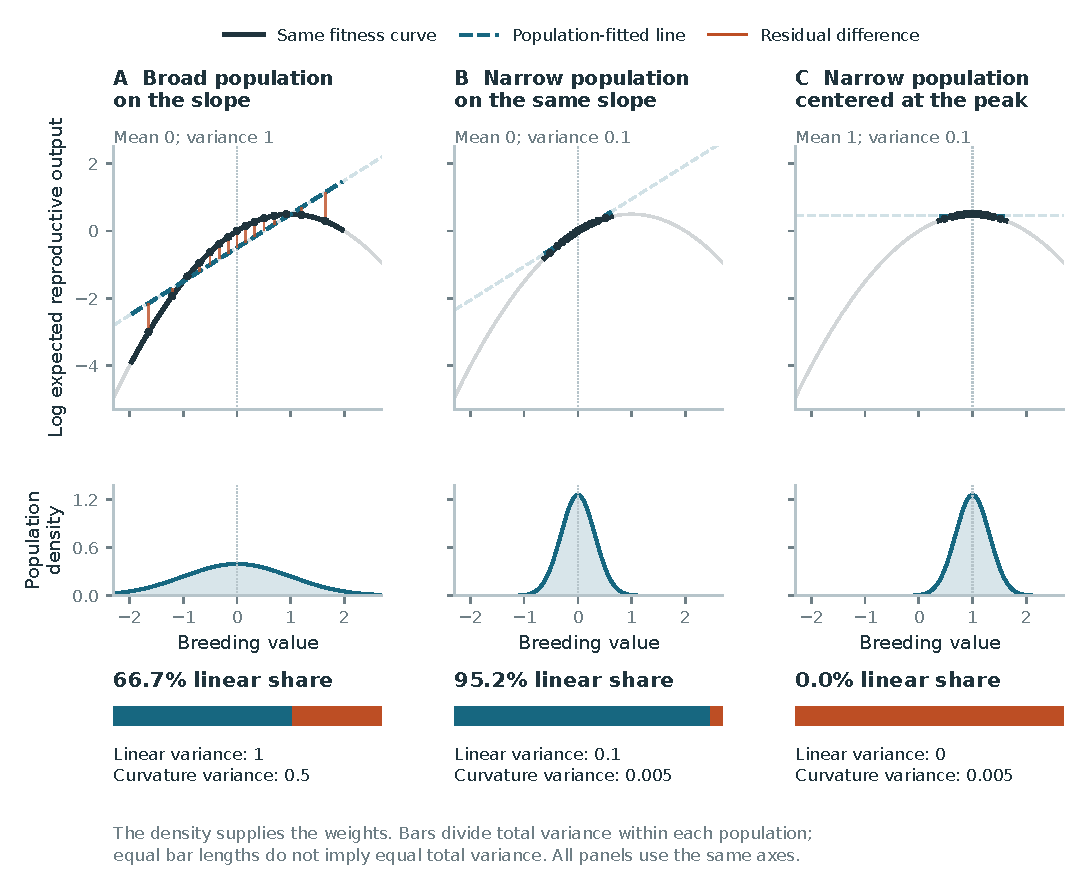
\includegraphics[width=\textwidth]{../one_trait_visual/figures/one_trait_additive_channel.pdf}
\caption{The curve is the same in all three populations. Population variance changes the weights assigned to its values; moving the mean to the peak also changes the local slope. The displayed densities are separate from the fitness scale. All values in the table are population calculations, not estimates from the plotted points.}
\label{worked:fig_one_trait}
\end{figure}

\paragraph{Biological interpretation.}
A narrow population has a large linear share in the second case because its mean is on the slope. Narrowness by itself does not give a large share: at the peak the first-order component vanishes while curvature still produces variation.

\section{Rotating the population on a fixed two-trait surface}
\label{worked:rotation}

The geometry example takes $\bGamma=0.8\mat I$ and an optimum whose original coordinates are $(0.9375,0.375)^{\mathsf T}$. An orthonormal coordinate change places the direction towards the optimum along the first axis. This preliminary relabelling does not change any variance component. The mean remains zero and the gradient is $(g,0)^{\mathsf T}$, where
\[
 g^2=(0.8)^2(0.9375^2+0.375^2)=0.6525.
\]
Now physically rotate the covariance, keeping the fitness surface and trait axes fixed:
\[
 \mat G_\varphi=\mat R_\varphi
 \begin{pmatrix}0.20&0\\0&0.005\end{pmatrix}
 \mat R_\varphi^{\mathsf T},\qquad
 \mat R_\varphi=
 \begin{pmatrix}\cos\varphi&-\sin\varphi\\
                 \sin\varphi&\cos\varphi\end{pmatrix}.
\]
Matrix multiplication gives
$G_{\varphi,11}=0.20\cos^2\varphi+0.005\sin^2\varphi$. Since only the first gradient coordinate is nonzero,
\begin{align}
 \Vlin(\varphi)&=0.6525\{0.20\cos^2\varphi+0.005\sin^2\varphi\},\\
 \Vquad(\varphi)&=\frac{0.8^2}{2}\tr(\mat G_\varphi^2)
 =\frac{0.8^2}{2}(0.20^2+0.005^2)=0.012808.
\end{align}
The second equality follows because rotation preserves the covariance eigenvalues, and the curvature is isotropic in this example. It need not hold for arbitrary curvature.

\begin{center}
\begin{tabular}{@{}lrrr@{}}
\toprule Rotation & $\Vlin$ & $\Vquad$ & $\Ag$\\
\midrule
$0^\circ$ &0.1305&0.012808&0.910626\\
$45^\circ$&0.06688125&0.012808&0.839276\\
$90^\circ$&0.0032625&0.012808&0.203012\\
\bottomrule
\end{tabular}
\end{center}
At $90^\circ$, the long axis is perpendicular to the gradient, but variance $0.005$ remains in the gradient direction. A section along the long axis therefore has zero first-order slope even though the full population has a positive linear component. A one-dimensional slice cannot replace the full two-trait calculation.

There is another angle in the teaching figures, defined between centred fitness functions under the inner product $\langle f,h\rangle=\E[fh]$. If both the linear component and total variance are positive, let $\psi$ be the angle between $L$ and $L+Q_c$. Orthogonality gives
\[
 \cos\psi
 =\frac{\E[L(L+Q_c)]}
 {\sqrt{\E[L^2]}\sqrt{\E[(L+Q_c)^2]}}
 =\sqrt{\frac{\Vlin}{\Vlin+\Vquad}},
 \qquad \Ag=\cos^2\psi.
\]
This angle is between functions, with the population supplying their inner product. It is not the physical rotation $\varphi$ of the covariance ellipse. When $L$ is the zero function, its ordinary angle is undefined; a drawn $90^\circ$ triangle then represents a limit.

\subsection{The same share from different population changes}
\label{worked:comparison}

The four geometry comparison cases alter covariance scale $s$ and the distance to the optimum by a factor $d$. With isotropic fixed curvature and the original direction to the optimum retained, the new gradient is $d\vect b_0$ and the new covariance is $s\mat G_0$. Hence
\[
 \Vlin(s,d)=sd^2L_0,\qquad
 \Vquad(s,d)=s^2Q_0,\qquad
 \Ag(s,d)=\frac{d^2L_0}{d^2L_0+sQ_0}.
\]
Case A has $(s,d)=(1,1)$ and gives $0.603954$. Case B has $(0.11,1)$ and gives $0.932720$. Case C has $(0.11,0)$ and gives zero. Case D has $(1,1/\sqrt{0.11})$, so
\[
 \Ag(1,1/\sqrt{0.11})
 =\frac{L_0/0.11}{L_0/0.11+Q_0}
 =\frac{L_0}{L_0+0.11Q_0}
 =\Ag(0.11,1).
\]
The identical shares in B and D describe different absolute components. B narrows the population. D retains its covariance and places its mean farther from the peak. The share alone does not identify which biological difference occurred.

\section{Reproductive contributions of a fixed sample of parents}
\label{worked:parental}

For a displayed sample of $n$ parents with known log conditional means $\ell_i$, the equal-frequency and expected-output weights are
\[
 q_i^{(0)}=\frac1n,\qquad
 q_i^{(W)}=\frac{\exp(\ell_i)}{\sum_j\exp(\ell_j)}.
\]
Fit an affine predictor $\widehat\ell_i$ using an intercept and all relevant breeding-value coordinates. The line-based reproductive weights are
$q_i^{(1)}=\exp(\widehat\ell_i)/\sum_j\exp(\widehat\ell_j)$.
For any specified group $S$, its population fraction is
$\sum_{i\in S}q_i^{(0)}$ and its expected reproductive fraction is
$\sum_{i\in S}q_i^{(W)}$. The difference is entirely a difference of weights on the same parents.

The two-trait companion recovers case 25 from the Main Figure 2 random stream and retains all 20,000 parents for calculation. The group is defined by a first-trait breeding value more than one sample standard deviation below its mean. It contains 3,180 parents, so its frequency is $3180/20000=0.159$. Its expected reproductive fraction under the curved relationship is $0.2846675$; the fitted plane assigns it $0.3412681$.

The displayed shifts standardise each coordinate by that trait's starting sample standard deviation. In this coordinate system the full shift has length $0.6380495$, whereas the plane-based shift has length $0.8299486$. The reported length overestimate is
\[
 \frac{0.8299486}{0.6380495}-1=0.3007591.
\]
This is a comparison of two shift lengths in the displayed coordinates. It is not the norm of their vector difference divided by the full shift, and the coordinatewise standardisation is not generally the $\mat G^{-1}$ norm used in Chapter~\ref{selection:chapter}. The example illustrates changed reproductive contributions without changing the definition of that theorem's error bound.

For the 800-genotype estimation example, realised counts $r_i$ give an additional set of weights,
$q_i^{(\mathrm{obs})}=r_i/\sum_jr_j$, provided total reproduction is positive. The sample has 2,862 offspring and 88 zero counts. For this teaching comparison, the group is defined from the separately saved true simulated breeding values: it includes values more than one sample standard deviation above their mean. The group contains 122 genotypes, with frequency $122/800=0.1525$, and contributes 585 observed offspring, a fraction $585/2862=0.2044025$. Its conditional expected fraction under the generating curve is approximately $0.212940$. The difference between those last two fractions is sampling variation in reproduction. The true breeding values and generating curve are used only to check this teaching comparison; they are not inputs to the estimator. None of these weighted parental distributions specifies offspring breeding values without a transmission model.

\section{The mathematics guide's recurring example}
\label{worked:guide}

The guide's five figures and eleven checkpoints use the preceding derivations with a small set of parameters. In its phenotype construction, $\theta=4$, $\omega^2=1$ and $V_E=1$. Conditional averaging gives
$\ell_A(a)=c-(a-4)^2/4$. At the reference mean zero this is
$\ell_0+2a-a^2/4$, with $b=2$ and $H=-0.5$. The following calculations make the numerical checks reproducible without reading values from a graph.

\subsection{Conditional averages and finite differences}

For outputs $(0,2)$ the conditional sample mean is 1 and its logarithm is zero. For $(1,3)$ the mean is 2 and its logarithm is $\log2$. The first group's mean of logged counts is not finite. These are checks on the order of operations, rather than estimates from the full teaching dataset.

For a quadratic polynomial $\ell_0+bx+Hx^2/2$,
\begin{align}
 \frac{\ell(\varepsilon)-\ell(-\varepsilon)}{2\varepsilon}
 &=\frac{2b\varepsilon}{2\varepsilon}=b,\\
 \frac{\ell(\varepsilon)-2\ell(0)+\ell(-\varepsilon)}{\varepsilon^2}
 &=\frac{H\varepsilon^2}{\varepsilon^2}=H.
\end{align}
With $\varepsilon=0.2$, the changes from $\ell_0$ are $0.39$ and $-0.41$.
The two finite differences are $0.80/0.40=2$ and $-0.02/0.04=-0.5$.
They are exact here because the function is quadratic; general smooth functions also have finite-difference approximation error.

\subsection{Components, units and selected-parent moments}

With $G=1$, the components are $b^2G=4$ and $H^2G^2/2=0.125$, so
$\Ag=4/4.125=32/33$. The centred quadratic term is
$Q_c=-0.25(x^2-1)$. At $x=2$ the product $LQ_c$ is $4(-0.75)=-3$; at
$x=-2$ it is $(-4)(-0.75)=3$. Equal Gaussian weights make these paired contributions cancel. Chapter~\ref{gaussian:chapter} establishes this for the whole distribution.

Changing trait units to $x'=10x$ gives $G'=100$, $b'=0.2$ and $H'=-0.005$.
Substitution gives $(0.2)^2(100)=4$ and
$(-0.005)^2(100)^2/2=0.125$, so neither component changes.

With $\Gamma=0.5$, selected variance is
$G_{\mathrm{sel}}=(1+0.5)^{-1}=2/3$ and selected-parent displacement is
$(2/3)2=4/3$. Ignoring curvature predicts displacement 2. Its relative error is
$(2-4/3)/(4/3)=1/2$. Replacing $b=2$ by $b=10$ changes the share to
$100/100.125=0.998752$, but the full and linear displacements become
$20/3$ and 10, retaining the same relative error $1/2$.

\subsection{Inheritance and phenotype-regression checkpoints}

The guide takes $B=1$, $\gamma=0.5$, $\rho=0.5$ and $g_0=1$. Iteration gives
\[
 g_1=\frac56,\qquad g_2=\frac{27}{34},\qquad
 g_3=\frac{149}{190},\qquad g_4=\frac{827}{1058}.
\]
The decimal values are $0.833333$, $0.794118$, $0.784211$ and $0.781664$.
Solving the scalar fixed-point equation gives $g^*=(\sqrt{17}-1)/4$.
With $\rho=1$ instead, $g_4^{-1}=g_0^{-1}+4\gamma=3$, so $g_4=1/3$.

The final checkpoint takes $P=1.5$, $\beta=0.4$, $\gamma=-0.2$ and $G=0.5$ in the raw relative-fitness regression convention. Here $\gamma$ denotes the regression coefficient, not the stabilising parameter in the preceding paragraph. Chapter~\ref{conversion:chapter} gives
\begin{align}
 \alpha&=1-\tfrac12(-0.2)(1.5)=1.15,\\
 G_{\mathrm{sel}}&=0.5+(0.5)^2\{-0.2-(0.4)^2\}=0.41,\\
 b&=\frac{0.5(0.4)}{0.41}=0.4878048780,\\
 H&=\frac1{0.5}-\frac1{0.41}=-0.4390243902.
\end{align}
The guide's tenth checkpoint concerns logical scope: a current-population approximation check is not a test of an inheritance recursion. The simulation calculation below explains why.

\section{The fitted estimation example}
\label{worked:estimation}

Chapter~\ref{estimation:chapter} derives the calibration, conditional likelihood and uncertainty procedure. The default example generates 800 genotypes with three independent noisy height observations per genotype and one reproductive count. Its generating parameters are $b=0.7$, $H=-0.7$ and $G=1$, giving
\[
 \Vlin=0.7^2=0.49,\qquad
 \Vquad=\frac{(-0.7)^2}{2}=0.245,\qquad
 \Ag=\frac{0.49}{0.735}=\frac23.
\]
The observation seed is $20261005$; the bootstrap seed is $20261006$.
The recorded results are:

\begin{center}
\small
\begin{tabular}{@{}lrrl@{}}
\toprule Quantity & Generating value & Estimate & Conditional 95\% interval\\
\midrule
$b$ &0.7&0.682560&$[0.600334,\;0.778885]$\\
$H$ &$-0.7$&$-0.769799$&$[-0.916719,\;-0.630133]$\\
$G$ &1&1.002149&$[0.876642,\;1.136257]$\\
$\Vlin$ &0.49&0.466889&$[0.354749,\;0.599602]$\\
$\Vquad$ &0.245&0.297570&$[0.195636,\;0.421178]$\\
$\Ag$ &$2/3$&0.610744&$[0.533024,\;0.685713]$\\
\bottomrule
\end{tabular}
\end{center}
The fitted measurement variance is $0.979881$ and the corresponding reliability is $0.754189$. Recalibrating and refitting all 500 bootstrap samples gives the stated intervals; no reference bootstrap fit failed. The naive analysis, which treats predictions as known breeding values and refits the fitness relationship, gives $0.673984$. It changes fitted slope and curvature as well as variance, so it is not the same experiment as substituting a smaller $G$ while holding $b,H$ fixed.

The three estimation figures display the observed counts and conditional mean, component estimates with bootstrap intervals, and observable-data diagnostics. For the default data, the quartic-minus-quadratic conditional AIC difference is $3.410883$. Raising quadrature order from 41 to 81 changes each of $b,H,\Ag$ by less than $4\times10^{-13}$ for this fit. These checks support this numerical calculation under its observation model; they do not prove that the model is correct.

The separate quartic generating example adds $-0.08a^4$. Its second derivative at the mean leaves the local quadratic share at $2/3$, while its full-curve affine $R^2$ is $0.242406$. The eighth-moment derivation in Chapter~\ref{estimation:chapter} accounts for that difference. Changing functional form and increasing numerical integration accuracy address different sources of error.

\section{What the multilocus simulation assesses}
\label{worked:simulation}

The simulation uses four additive traits and Gaussian stabilising selection,
$\ell(\vect a)=-\tfrac12(\vect a-\vect\theta)^{\mathsf T}
\bGamma(\vect a-\vect\theta)$, with
$\bGamma=\operatorname{diag}(0.10,0.05,0.04,0.03)$.
At each generation, set $\vect x_i=\vect a_i-\bar{\vect a}$ and expand:
\[
 \ell(\bar{\vect a}+\vect x_i)
 =\ell(\bar{\vect a})
 +\{\bGamma(\vect\theta-\bar{\vect a})\}^{\mathsf T}\vect x_i
 -\frac12\vect x_i^{\mathsf T}\bGamma\vect x_i .
\]
Thus $\vect b=\bGamma(\vect\theta-\bar{\vect a})$ and $\mat H=-\bGamma$ are known exactly for that generation's mean. The analysis estimates covariance using
$\widehat{\mat G}=(N-1)^{-1}\sum_i\vect x_i\vect x_i^{\mathsf T}$,
inserts it into the Gaussian component formulas, and compares the resulting share with Equation~\eqref{worked:sample_r2} for the observed finite population.

Each of 20 replicates has $N=2000$, 200 loci (50 per trait) and 200 recorded generations. Allelic-effect standard deviations are
$(0.346,0.283,0.200,0.141)$. The first optimum coordinate increases by 0.3 per generation for 40 generations to 12, then remains fixed; the other coordinates remain zero. No environmental residual is added. Seeds 42--61 define the replicate runs.

For replicate $r$ and generation $t$, let
$d_{rt}=|\widehat{\Ag}_{rt}-r_{rt}^2|$. The reported statistic is the median of the $20\times200=4000$ values, namely $0.0156678857$. A table of those diagnostic values is sufficient to reproduce that summary. Recreating every individual population instead requires the SLiM model, version and seed sequence; these are provided separately in the repository.

The polynomial expansion remains exact for these individuals, but their finite breeding-value distribution need not be Gaussian. Their third and fourth moments, and finite-sample estimation, can therefore produce a discrepancy between the Gaussian component formula and the sample squared correlation. This correlation uses the theoretical linear term; it is not necessarily the best unrestricted multivariate affine fit to a non-Gaussian sample. Chapter~\ref{gaussian:chapter} gives the general moment terms that the Gaussian simplification removes.

\paragraph{Biological interpretation.}
The comparison assesses a current-population approximation in a multilocus design. Allele frequencies and associations change during that simulation. Its agreement with the variance formula consequently cannot validate the separate recursion that holds $\mat B$ fixed. It also does not test the selected-parent displacement bound unless that additional comparison is explicitly computed.

\section{Reproducing the numerical work}
\label{worked:commands}

From the repository root, the principal commands are
\begin{verbatim}
bash run_all.sh --quick
bash run_all.sh
bash run_all.sh --visuals
bash run_all.sh --simulate
bash run_shiny.sh
\end{verbatim}
The first regenerates the main figures, mathematical checks and archived simulation summary. The second adds the fitted estimation example and all 500 bootstrap refits. The third rebuilds the visual examples and offline explorers. The fourth runs fresh simulations and requires SLiM 5.2. The final command starts the Shiny app, which uses the same model and analysis code as the batch estimation example.

The \repofile{RESULTS.md}{result catalogue} and
\repofile{REPRODUCING.md}{reproduction guide} identify exact inputs and outputs.
The two offline explorers calculate the same Gaussian geometry or sample reproductive weights derived above. Changing an app control specifies a new example; it does not introduce a new theorem. The figures, observation model and proof assumptions should be interpreted together.

\appendix
\chapter{Result-by-result derivation map}\label{coverage:chapter}

This map covers all 53 records in the existing result catalogue. Some describe the same mathematics at different locations, and some describe figures, estimation procedures or teaching resources. They are not 53 distinct theorems. Each link goes to the appropriate proof or calculation.

\section{Analytical results, examples and resources}

\small\begin{longtable}{@{}p{0.60\textwidth}p{0.32\textwidth}@{}}

\toprule Result or resource & Derivation or calculation\\\midrule\endhead

Main Figure 1: Construct conditional expected fitness before taking logs\newline{\footnotesize\itshape Worked or numerical calculation} & \hyperref[worked:main1]{p.~\pageref*{worked:main1}}; \hyperref[conditioning:environmental_average]{p.~\pageref*{conditioning:environmental_average}}\\[4pt]

Main Figure 2: Gaussian population projection identity\newline{\footnotesize\itshape Worked or numerical calculation} & \hyperref[gaussian:affine_projection]{p.~\pageref*{gaussian:affine_projection}}; \hyperref[worked:main2]{p.~\pageref*{worked:main2}}\\[4pt]

Main Figure 3: Proportional covariance contraction on a fixed surface\newline{\footnotesize\itshape Worked or numerical calculation} & \hyperref[geometry:scaling]{p.~\pageref*{geometry:scaling}}; \hyperref[worked:main3]{p.~\pageref*{worked:main3}}\\[4pt]

Main Figure 4: Scalar covariance trajectory with a separately changing gradient\newline{\footnotesize\itshape Worked or numerical calculation} & \hyperref[inheritance:scalar]{p.~\pageref*{inheritance:scalar}}; \hyperref[worked:main4]{p.~\pageref*{worked:main4}}\\[4pt]

Conditional mean, logarithm and reproductive weighting\newline{\footnotesize\itshape Analytical derivation} & \hyperref[conditioning:target]{p.~\pageref*{conditioning:target}}; \hyperref[conditioning:selection_weight]{p.~\pageref*{conditioning:selection_weight}}; \hyperref[conditioning:jensen]{p.~\pageref*{conditioning:jensen}}\\[4pt]

Gaussian environmental averaging changes breeding-value curvature\newline{\footnotesize\itshape Analytical derivation} & \hyperref[conditioning:environmental_average]{p.~\pageref*{conditioning:environmental_average}}; \hyperref[worked:main1]{p.~\pageref*{worked:main1}}\\[4pt]

Local quadratic approximation and the full nonquadratic curve\newline{\footnotesize\itshape Analytical derivation} & \hyperref[gaussian:taylor_derivation]{p.~\pageref*{gaussian:taylor_derivation}}; \hyperref[estimation:quartic_centring]{p.~\pageref*{estimation:quartic_centring}}\\[4pt]

Linear and centred-quadratic Gaussian moments\newline{\footnotesize\itshape Analytical derivation} & \hyperref[gaussian:moments]{p.~\pageref*{gaussian:moments}}; \hyperref[gaussian:variance_derivation]{p.~\pageref*{gaussian:variance_derivation}}\\[4pt]

Affine regression intercept, slope and R\textsuperscript{2}\newline{\footnotesize\itshape Analytical derivation} & \hyperref[gaussian:projection_section]{p.~\pageref*{gaussian:projection_section}}\\[4pt]

Noise reduces both R\textsuperscript{2} values but their ratio recovers the share\newline{\footnotesize\itshape Analytical derivation} & \hyperref[conditioning:log_gap_model]{p.~\pageref*{conditioning:log_gap_model}}; \hyperref[gaussian:noisy_response]{p.~\pageref*{gaussian:noisy_response}}\\[4pt]

Proportional covariance scaling and the omitted fraction\newline{\footnotesize\itshape Analytical derivation} & \hyperref[geometry:scaling]{p.~\pageref*{geometry:scaling}}; \hyperref[worked:main3]{p.~\pageref*{worked:main3}}\\[4pt]

A smaller covariance can reduce the linear share\newline{\footnotesize\itshape Explicit counterexample} & \hyperref[geometry:anisotropic_counterexample]{p.~\pageref*{geometry:anisotropic_counterexample}}\\[4pt]

Changing trait units leaves the component variances unchanged\newline{\footnotesize\itshape Analytical derivation} & \hyperref[geometry:coordinate_change]{p.~\pageref*{geometry:coordinate_change}}\\[4pt]

Whitening, curvature eigenvalues and the separate Rayleigh quotient\newline{\footnotesize\itshape Analytical derivation} & \hyperref[geometry:whitening]{p.~\pageref*{geometry:whitening}}; \hyperref[geometry:physical_orientation]{p.~\pageref*{geometry:physical_orientation}}; \hyperref[worked:rotation]{p.~\pageref*{worked:rotation}}\\[4pt]

Zero terms, undefined correlation and singular covariance support\newline{\footnotesize\itshape Analytical derivation} & \hyperref[gaussian:share]{p.~\pageref*{gaussian:share}}; \hyperref[gaussian:singular_support]{p.~\pageref*{gaussian:singular_support}}\\[4pt]

Asymmetry and non-Gaussian fourth moments can change the partition\newline{\footnotesize\itshape Analytical derivation} & \hyperref[gaussian:non_gaussian]{p.~\pageref*{gaussian:non_gaussian}}\\[4pt]

Exact selected-parent mean and covariance\newline{\footnotesize\itshape Analytical derivation} & \hyperref[selection:integrability]{p.~\pageref*{selection:integrability}}; \hyperref[selection:complete_square]{p.~\pageref*{selection:complete_square}}; \hyperref[selection:normaliser]{p.~\pageref*{selection:normaliser}}; \hyperref[selection:selected_moments]{p.~\pageref*{selection:selected_moments}}\\[4pt]

A large share does not ensure an accurate parental shift or perfect rankings\newline{\footnotesize\itshape Explicit counterexample} & \hyperref[selection:linear_comparison]{p.~\pageref*{selection:linear_comparison}}; \hyperref[selection:97_50_example]{p.~\pageref*{selection:97_50_example}}; \hyperref[worked:guide]{p.~\pageref*{worked:guide}}\\[4pt]

Absolute covariance-weighted curvature bounds relative displacement error\newline{\footnotesize\itshape Analytical derivation} & \hyperref[selection:error_bound_section]{p.~\pageref*{selection:error_bound_section}}; \hyperref[selection:eigenbasis_error]{p.~\pageref*{selection:eigenbasis_error}}\\[4pt]

Fixed allelic effects do not imply fixed genic covariance\newline{\footnotesize\itshape Analytical derivation} & \hyperref[inheritance:genic]{p.~\pageref*{inheritance:genic}}\\[4pt]

Fixed-baseline covariance interval and matrix fixed-point bounds\newline{\footnotesize\itshape Analytical derivation} & \hyperref[inheritance:matrix-order]{p.~\pageref*{inheritance:matrix-order}}; \hyperref[inheritance:matrix-fixed-point]{p.~\pageref*{inheritance:matrix-fixed-point}}\\[4pt]

Scalar fixed point, contraction and a transient increase\newline{\footnotesize\itshape Analytical derivation} & \hyperref[inheritance:scalar]{p.~\pageref*{inheritance:scalar}}; \hyperref[inheritance:scalar-boundaries]{p.~\pageref*{inheritance:scalar-boundaries}}\\[4pt]

No-restoration boundary and retained null-space variation\newline{\footnotesize\itshape Analytical derivation} & \hyperref[inheritance:rho-one]{p.~\pageref*{inheritance:rho-one}}\\[4pt]

Prediction shrinkage can mimic proportional biological contraction\newline{\footnotesize\itshape Analytical derivation} & \hyperref[estimation:conditioning]{p.~\pageref*{estimation:conditioning}}; \hyperref[estimation:shrinkage]{p.~\pageref*{estimation:shrinkage}}\\[4pt]

Convert compatible phenotype regression moments to breeding-value parameters\newline{\footnotesize\itshape Analytical derivation} & \hyperref[conversion:regression]{p.~\pageref*{conversion:regression}}; \hyperref[conversion:phenotype_moments]{p.~\pageref*{conversion:phenotype_moments}}; \hyperref[conversion:breeding_moments]{p.~\pageref*{conversion:breeding_moments}}; \hyperref[conversion:inversion]{p.~\pageref*{conversion:inversion}}\\[4pt]

Appendix S1: Gaussian moments and population projections\newline{\footnotesize\itshape Analytical derivation} & \hyperref[gaussian:chapter]{Chapter~\ref*{gaussian:chapter}}; \hyperref[geometry:chapter]{Chapter~\ref*{geometry:chapter}}\\[4pt]

Appendix S2: Gaussian selection, environmental averaging and displacement bound\newline{\footnotesize\itshape Analytical derivation} & \hyperref[conditioning:environmental_average]{p.~\pageref*{conditioning:environmental_average}}; \hyperref[selection:integrability]{p.~\pageref*{selection:integrability}}; \hyperref[selection:selected_moments]{p.~\pageref*{selection:selected_moments}}; \hyperref[selection:error_bound_section]{p.~\pageref*{selection:error_bound_section}}\\[4pt]

Appendix S3: Fixed-baseline inheritance and its limits\newline{\footnotesize\itshape Analytical derivation} & \hyperref[inheritance:chapter]{Chapter~\ref*{inheritance:chapter}}\\[4pt]

Appendix S4: Forward-time finite-population approximation\newline{\footnotesize\itshape Worked or numerical calculation} & \hyperref[worked:simulation]{p.~\pageref*{worked:simulation}}\\[4pt]

Appendix S5: Moment conversion from phenotype regressions\newline{\footnotesize\itshape Analytical derivation} & \hyperref[conversion:chapter]{Chapter~\ref*{conversion:chapter}}\\[4pt]

Appendix S6: Interpretation, assumptions and boundaries\newline{\footnotesize\itshape Interpretation} & \hyperref[coverage:questions]{p.~\pageref*{coverage:questions}}; \hyperref[concepts:chapter]{Chapter~\ref*{concepts:chapter}}\\[4pt]

Appendix S7: Visual one-trait and rotation examples\newline{\footnotesize\itshape Worked or numerical calculation} & \hyperref[worked:one_trait]{p.~\pageref*{worked:one_trait}}; \hyperref[worked:rotation]{p.~\pageref*{worked:rotation}}\\[4pt]

SLiM approximation check over 4,000 generation records\newline{\footnotesize\itshape Worked or numerical calculation} & \hyperref[worked:simulation]{p.~\pageref*{worked:simulation}}\\[4pt]

One fixed curve with broad, narrow and peak-centred populations\newline{\footnotesize\itshape Worked or numerical calculation} & \hyperref[worked:one_trait]{p.~\pageref*{worked:one_trait}}\\[4pt]

Rotate the same covariance eigenvalues on a fixed surface\newline{\footnotesize\itshape Worked or numerical calculation} & \hyperref[worked:rotation]{p.~\pageref*{worked:rotation}}\\[4pt]

Average phenotype-dependent expected output at each breeding value\newline{\footnotesize\itshape Worked or numerical calculation} & \hyperref[conditioning:environmental_average]{p.~\pageref*{conditioning:environmental_average}}; \hyperref[worked:guide]{p.~\pageref*{worked:guide}}\\[4pt]

Compare the linear and centred quadratic contributions\newline{\footnotesize\itshape Worked or numerical calculation} & \hyperref[gaussian:variance_derivation]{p.~\pageref*{gaussian:variance_derivation}}; \hyperref[worked:guide]{p.~\pageref*{worked:guide}}\\[4pt]

Reproductive weighting gives a selected-parent distribution\newline{\footnotesize\itshape Worked or numerical calculation} & \hyperref[selection:linear_comparison]{p.~\pageref*{selection:linear_comparison}}; \hyperref[selection:97_50_example]{p.~\pageref*{selection:97_50_example}}; \hyperref[worked:guide]{p.~\pageref*{worked:guide}}\\[4pt]

Iterate the scalar covariance closure\newline{\footnotesize\itshape Worked or numerical calculation} & \hyperref[inheritance:guide-fixed-point]{p.~\pageref*{inheritance:guide-fixed-point}}; \hyperref[worked:guide]{p.~\pageref*{worked:guide}}\\[4pt]

From phenotype moments to log conditional-fitness parameters\newline{\footnotesize\itshape Worked or numerical calculation} & \hyperref[conversion:scalar_example]{p.~\pageref*{conversion:scalar_example}}; \hyperref[worked:guide]{p.~\pageref*{worked:guide}}\\[4pt]

Every numerical checkpoint and the multivariate extension\newline{\footnotesize\itshape Worked or numerical calculation} & \hyperref[worked:guide]{p.~\pageref*{worked:guide}}; \hyperref[gaussian:chapter]{Chapter~\ref*{gaussian:chapter}}; \hyperref[selection:chapter]{Chapter~\ref*{selection:chapter}}; \hyperref[inheritance:chapter]{Chapter~\ref*{inheritance:chapter}}; \hyperref[conversion:chapter]{Chapter~\ref*{conversion:chapter}}\\[4pt]

Two-stage estimation from repeated measurements and offspring counts\newline{\footnotesize\itshape Statistical procedure} & \hyperref[estimation:calibration]{p.~\pageref*{estimation:calibration}}; \hyperref[estimation:likelihood]{p.~\pageref*{estimation:likelihood}}; \hyperref[estimation:components]{p.~\pageref*{estimation:components}}; \hyperref[worked:estimation]{p.~\pageref*{worked:estimation}}\\[4pt]

Joint refitting and model-conditional uncertainty\newline{\footnotesize\itshape Statistical procedure} & \hyperref[estimation:bootstrap]{p.~\pageref*{estimation:bootstrap}}; \hyperref[worked:estimation]{p.~\pageref*{worked:estimation}}\\[4pt]

Latent integration, recovery and explicit numerical failures\newline{\footnotesize\itshape Statistical procedure} & \hyperref[estimation:quadrature]{p.~\pageref*{estimation:quadrature}}; \hyperref[estimation:score]{p.~\pageref*{estimation:score}}; \hyperref[estimation:integration_check]{p.~\pageref*{estimation:integration_check}}\\[4pt]

Model shape, diagnostics and the local-versus-full distinction\newline{\footnotesize\itshape Analytical derivation} & \hyperref[estimation:aic]{p.~\pageref*{estimation:aic}}; \hyperref[estimation:quartic_centring]{p.~\pageref*{estimation:quartic_centring}}; \hyperref[estimation:quartic]{p.~\pageref*{estimation:quartic}}; \hyperref[worked:estimation]{p.~\pageref*{worked:estimation}}\\[4pt]

Observed counts and latent conditional relationship\newline{\footnotesize\itshape Statistical procedure} & \hyperref[estimation:components]{p.~\pageref*{estimation:components}}; \hyperref[estimation:predictions]{p.~\pageref*{estimation:predictions}}; \hyperref[worked:estimation]{p.~\pageref*{worked:estimation}}\\[4pt]

Component estimates, naive comparison and conditional interval\newline{\footnotesize\itshape Statistical procedure} & \hyperref[estimation:bootstrap]{p.~\pageref*{estimation:bootstrap}}; \hyperref[worked:estimation]{p.~\pageref*{worked:estimation}}\\[4pt]

Observable-bin predictions and zero-count checks\newline{\footnotesize\itshape Statistical procedure} & \hyperref[estimation:predictions]{p.~\pageref*{estimation:predictions}}; \hyperref[estimation:bin_variance]{p.~\pageref*{estimation:bin_variance}}; \hyperref[estimation:quartic]{p.~\pageref*{estimation:quartic}}\\[4pt]

Runnable scientific source, reference data and result checks\newline{\footnotesize\itshape Reproduction resource} & \hyperref[worked:commands]{p.~\pageref*{worked:commands}}; \hyperref[coverage:commands]{p.~\pageref*{coverage:commands}}\\[4pt]

Observation means, population-fitted lines and parental shift\newline{\footnotesize\itshape Worked or numerical calculation} & \hyperref[conditioning:chapter]{Chapter~\ref*{conditioning:chapter}}; \hyperref[worked:one_trait]{p.~\pageref*{worked:one_trait}}; \hyperref[worked:guide]{p.~\pageref*{worked:guide}}\\[4pt]

Rotate, narrow or move a Gaussian population on one fixed surface\newline{\footnotesize\itshape Worked or numerical calculation} & \hyperref[geometry:chapter]{Chapter~\ref*{geometry:chapter}}; \hyperref[worked:rotation]{p.~\pageref*{worked:rotation}}; \hyperref[worked:comparison]{p.~\pageref*{worked:comparison}}\\[4pt]

Frequency, expected-output and recorded-count weights\newline{\footnotesize\itshape Worked or numerical calculation} & \hyperref[conditioning:selection_weight]{p.~\pageref*{conditioning:selection_weight}}; \hyperref[worked:parental]{p.~\pageref*{worked:parental}}\\[4pt]

Change measurement uncertainty, sample size and model shape\newline{\footnotesize\itshape Reproduction resource} & \hyperref[estimation:likelihood]{p.~\pageref*{estimation:likelihood}}; \hyperref[estimation:predictions]{p.~\pageref*{estimation:predictions}}; \hyperref[estimation:bootstrap]{p.~\pageref*{estimation:bootstrap}}; \hyperref[worked:commands]{p.~\pageref*{worked:commands}}\\[4pt]

\bottomrule\end{longtable}\normalsize

\section{Equation-by-equation map}\label{coverage:equations}

The following 106 source-qualified equation identifiers connect the main account and supplementary derivations to this companion. These are stable source labels, not printed equation numbers. The same label can occur in different sources. Definitions and model assumptions are identified separately from proofs and worked calculations. The source versions inspected on 2026-11-13 are identified by hashes in \repofile{tutorials/derivations/equation_map.json}{the equation map}. The map contains identifiers and concepts; the source documents are not needed to build this companion.

\Needspace{8\baselineskip}

\subsection{Main text and mathematical appendices}

\small\begin{longtable}{@{}>{\raggedright\arraybackslash}p{0.28\textwidth}>{\raggedright\arraybackslash}p{0.47\textwidth}>{\raggedright\arraybackslash}p{0.16\textwidth}@{}}

\toprule Source label & Concept and treatment & Derivation\\\midrule\endhead

\codepath{eq:target} & Conditional expected reproduction and its logarithm\newline{\footnotesize\itshape definition} & \hyperref[conditioning:target]{p.~\pageref*{conditioning:target}}; \hyperref[conditioning:log_target]{p.~\pageref*{conditioning:log_target}}\\[4pt]

\codepath{eq:selection_weight} & Normalised reproductive weighting of parental frequencies\newline{\footnotesize\itshape proof + definition} & \hyperref[conditioning:selection_weight]{p.~\pageref*{conditioning:selection_weight}}; \hyperref[conditioning:selected_density]{p.~\pageref*{conditioning:selected_density}}\\[4pt]

\codepath{eq:log_ratio} & Log differences as proportional changes in conditional mean output\newline{\footnotesize\itshape proof} & \hyperref[conditioning:log_ratio]{p.~\pageref*{conditioning:log_ratio}}\\[4pt]

\codepath{eq:jensen} & Noncommutation of averaging and taking logarithms\newline{\footnotesize\itshape proof} & \hyperref[conditioning:jensen]{p.~\pageref*{conditioning:jensen}}; \hyperref[conditioning:jensen_inequality]{p.~\pageref*{conditioning:jensen_inequality}}\\[4pt]

\codepath{eq:taylor} & Local quadratic expansion of log conditional expected output\newline{\footnotesize\itshape definition + proof} & \hyperref[gaussian:quadratic_definition]{p.~\pageref*{gaussian:quadratic_definition}}; \hyperref[gaussian:taylor_derivation]{p.~\pageref*{gaussian:taylor_derivation}}\\[4pt]

\codepath{eq:centered_terms} & Mean-centred quadratic component\newline{\footnotesize\itshape definition + proof} & \hyperref[gaussian:terms]{p.~\pageref*{gaussian:terms}}; \hyperref[gaussian:quadratic_mean]{p.~\pageref*{gaussian:quadratic_mean}}\\[4pt]

\codepath{eq:vlin} & Variance of the linear component\newline{\footnotesize\itshape proof} & \hyperref[gaussian:linear_variance]{p.~\pageref*{gaussian:linear_variance}}\\[4pt]

\codepath{eq:vquad} & Gaussian variance of the quadratic component\newline{\footnotesize\itshape proof} & \hyperref[gaussian:four_index_variance]{p.~\pageref*{gaussian:four_index_variance}}; \hyperref[gaussian:quadratic_variance]{p.~\pageref*{gaussian:quadratic_variance}}\\[4pt]

\codepath{eq:Ag} & First-order share of quadratic log-target variance\newline{\footnotesize\itshape definition} & \hyperref[gaussian:share]{p.~\pageref*{gaussian:share}}; \hyperref[gaussian:variance_partition]{p.~\pageref*{gaussian:variance_partition}}\\[4pt]

\codepath{eq:affine_projection} & Population affine projection and curvature-adjusted intercept\newline{\footnotesize\itshape proof} & \hyperref[gaussian:affine_projection]{p.~\pageref*{gaussian:affine_projection}}; \hyperref[gaussian:fitted_affine]{p.~\pageref*{gaussian:fitted_affine}}\\[4pt]

\codepath{eq:r2_identity} & Regression and squared-correlation interpretations of the share\newline{\footnotesize\itshape proof} & \hyperref[gaussian:regression_share]{p.~\pageref*{gaussian:regression_share}}; \hyperref[gaussian:correlation_identity]{p.~\pageref*{gaussian:correlation_identity}}\\[4pt]

\codepath{eq:nested_r2} & Ratio of nested fit statistics and the complementary fraction\newline{\footnotesize\itshape proof} & \hyperref[gaussian:nested_r2]{p.~\pageref*{gaussian:nested_r2}}; \hyperref[gaussian:nested_ratio]{p.~\pageref*{gaussian:nested_ratio}}\\[4pt]

\codepath{eq:scaling} & Linear and quadratic components under proportional covariance scaling\newline{\footnotesize\itshape proof} & \hyperref[geometry:scaling_proposition]{p.~\pageref*{geometry:scaling_proposition}}; \hyperref[geometry:component_scaling]{p.~\pageref*{geometry:component_scaling}}\\[4pt]

\codepath{eq:whitening} & Gradient and Hessian in population-standardised coordinates\newline{\footnotesize\itshape definition + proof} & \hyperref[geometry:whitened_coefficients]{p.~\pageref*{geometry:whitened_coefficients}}; \hyperref[geometry:spectral_components]{p.~\pageref*{geometry:spectral_components}}\\[4pt]

\codepath{eq:log_quadratic_weight} & Exact quadratic reproductive-weight model\newline{\footnotesize\itshape definition} & \hyperref[selection:model]{p.~\pageref*{selection:model}}; \hyperref[selection:log_quadratic_weight]{p.~\pageref*{selection:log_quadratic_weight}}\\[4pt]

\codepath{eq:selected_mean} & Exact selected-parent mean displacement\newline{\footnotesize\itshape proof} & \hyperref[selection:selected_moments]{p.~\pageref*{selection:selected_moments}}; \hyperref[selection:moment_formulas]{p.~\pageref*{selection:moment_formulas}}\\[4pt]

\codepath{eq:selected_covariance} & Exact covariance under parental reproductive weights\newline{\footnotesize\itshape proof} & \hyperref[selection:selected_moments]{p.~\pageref*{selection:selected_moments}}; \hyperref[selection:moment_formulas]{p.~\pageref*{selection:moment_formulas}}\\[4pt]

\codepath{eq:counterexample} & Large variance share with a one-half displacement overestimate\newline{\footnotesize\itshape calculation} & \hyperref[selection:97_50_example]{p.~\pageref*{selection:97_50_example}}; \hyperref[worked:guide]{p.~\pageref*{worked:guide}}\\[4pt]

\codepath{eq:T} & Population-scaled stabilising curvature\newline{\footnotesize\itshape definition} & \hyperref[selection:T]{p.~\pageref*{selection:T}}; \hyperref[selection:precision_factorisation]{p.~\pageref*{selection:precision_factorisation}}\\[4pt]

\codepath{eq:response_bound} & Covariance-scaled relative displacement-error bound\newline{\footnotesize\itshape proof} & \hyperref[selection:relative_bound]{p.~\pageref*{selection:relative_bound}}; \hyperref[selection:full_bound]{p.~\pageref*{selection:full_bound}}\\[4pt]

\codepath{eq:fixedB_recursion} & Covariance update under fixed genic baseline and association retention\newline{\footnotesize\itshape definition + proof} & \hyperref[inheritance:retention-assumption]{p.~\pageref*{inheritance:retention-assumption}}; \hyperref[inheritance:recursion]{p.~\pageref*{inheritance:recursion}}\\[4pt]

\codepath{eq:genic_baseline} & Genic covariance from allele frequencies and fixed allelic effects\newline{\footnotesize\itshape proof} & \hyperref[inheritance:genic-formula]{p.~\pageref*{inheritance:genic-formula}}; \hyperref[inheritance:association-decomposition]{p.~\pageref*{inheritance:association-decomposition}}\\[4pt]

\codepath{eq:loewner_interval} & Invariant order interval for the covariance map\newline{\footnotesize\itshape definition + proof} & \hyperref[inheritance:interval]{p.~\pageref*{inheritance:interval}}; \hyperref[inheritance:invariance]{p.~\pageref*{inheritance:invariance}}\\[4pt]

\codepath{eq:fixedpoint_bounds} & Bounds on every positive covariance fixed point\newline{\footnotesize\itshape proof} & \hyperref[inheritance:existence]{p.~\pageref*{inheritance:existence}}; \hyperref[inheritance:fixed-bounds]{p.~\pageref*{inheritance:fixed-bounds}}\\[4pt]

\codepath{eq:scalar_recursion} & One-trait or isotropic covariance update\newline{\footnotesize\itshape definition + proof} & \hyperref[inheritance:scalar-map]{p.~\pageref*{inheritance:scalar-map}}; \hyperref[inheritance:scalar]{p.~\pageref*{inheritance:scalar}}\\[4pt]

\codepath{eq:scalar_root} & Unique positive scalar covariance fixed point\newline{\footnotesize\itshape proof} & \hyperref[inheritance:scalar-quadratic]{p.~\pageref*{inheritance:scalar-quadratic}}; \hyperref[inheritance:positive-root]{p.~\pageref*{inheritance:positive-root}}\\[4pt]

\codepath{eq:rho_one} & Precision accumulation with complete association retention\newline{\footnotesize\itshape proof} & \hyperref[inheritance:precision-iteration]{p.~\pageref*{inheritance:precision-iteration}}; \hyperref[inheritance:rho-one]{p.~\pageref*{inheritance:rho-one}}\\[4pt]

\codepath{eq:log_error_model} & Observation model with a constant conditional log gap\newline{\footnotesize\itshape definition + proof} & \hyperref[conditioning:constant_gap]{p.~\pageref*{conditioning:constant_gap}}; \hyperref[gaussian:noise_model]{p.~\pageref*{gaussian:noise_model}}\\[4pt]

\codepath{eq:ebv_inflation} & Share after substituting shrunken prediction covariance\newline{\footnotesize\itshape proof} & \hyperref[estimation:shrinkage_formula]{p.~\pageref*{estimation:shrinkage_formula}}; \hyperref[estimation:shrinkage_share]{p.~\pageref*{estimation:shrinkage_share}}\\[4pt]

\codepath{eq:LA_regression} & Raw relative-fitness phenotype regression and quadratic convention\newline{\footnotesize\itshape definition} & \hyperref[conversion:regression_model]{p.~\pageref*{conversion:regression_model}}; \hyperref[conversion:coefficient_convention]{p.~\pageref*{conversion:coefficient_convention}}\\[4pt]

\codepath{eq:LA_conversion} & Conversion of selected moments into log-quadratic parameters\newline{\footnotesize\itshape proof} & \hyperref[conversion:selected_formula]{p.~\pageref*{conversion:selected_formula}}; \hyperref[conversion:conversion_formula]{p.~\pageref*{conversion:conversion_formula}}\\[4pt]

\codepath{eq:fitness_model} & Phenotype-fitness model with independent Gaussian environment\newline{\footnotesize\itshape definition} & \hyperref[conditioning:phenotype_fitness]{p.~\pageref*{conditioning:phenotype_fitness}}; \hyperref[conditioning:environmental_average]{p.~\pageref*{conditioning:environmental_average}}\\[4pt]

\codepath{eq:environmental_average} & Gaussian environmental convolution of the fitness curve\newline{\footnotesize\itshape proof} & \hyperref[conditioning:environment_formula]{p.~\pageref*{conditioning:environment_formula}}; \hyperref[conditioning:environmental_average]{p.~\pageref*{conditioning:environmental_average}}\\[4pt]

\codepath{eq:precision_order} & Inverse-order covariance contraction under stabilising curvature\newline{\footnotesize\itshape proof} & \hyperref[inheritance:inverse-order]{p.~\pageref*{inheritance:inverse-order}}; \hyperref[inheritance:selection-order]{p.~\pageref*{inheritance:selection-order}}\\[4pt]

\codepath{eq:LA_moments} & Phenotype-regression normalisation and selected moments\newline{\footnotesize\itshape proof} & \hyperref[conversion:regression_moments]{p.~\pageref*{conversion:regression_moments}}; \hyperref[conversion:phenotype_moment_formula]{p.~\pageref*{conversion:phenotype_moment_formula}}\\[4pt]

\codepath{eq:LA_selected_mean} & Selected breeding-value mean from phenotype regression\newline{\footnotesize\itshape proof} & \hyperref[conversion:selected_breeding_moments]{p.~\pageref*{conversion:selected_breeding_moments}}; \hyperref[conversion:selected_formula]{p.~\pageref*{conversion:selected_formula}}\\[4pt]

\codepath{eq:LA_selected_cov} & Selected breeding-value covariance from phenotype regression\newline{\footnotesize\itshape proof} & \hyperref[conversion:selected_breeding_moments]{p.~\pageref*{conversion:selected_breeding_moments}}; \hyperref[conversion:selected_formula]{p.~\pageref*{conversion:selected_formula}}\\[4pt]

\bottomrule\end{longtable}\normalsize

\Needspace{8\baselineskip}

\subsection{Appendix S7: visual walkthrough}

\small\begin{longtable}{@{}>{\raggedright\arraybackslash}p{0.28\textwidth}>{\raggedright\arraybackslash}p{0.47\textwidth}>{\raggedright\arraybackslash}p{0.16\textwidth}@{}}

\toprule Source label & Concept and treatment & Derivation\\\midrule\endhead

\codepath{eq:visual_model} & Fixed one-trait curve and Gaussian populations\newline{\footnotesize\itshape definition} & \hyperref[worked:one_trait]{p.~\pageref*{worked:one_trait}}\\[4pt]

\codepath{eq:visual_variances} & Variance components for the three one-trait populations\newline{\footnotesize\itshape calculation + proof} & \hyperref[worked:one_trait]{p.~\pageref*{worked:one_trait}}; \hyperref[gaussian:variance_formulas]{p.~\pageref*{gaussian:variance_formulas}}\\[4pt]

\codepath{eq:visual_line} & Population-fitted line for the one-trait walkthrough\newline{\footnotesize\itshape calculation + proof} & \hyperref[worked:one_trait]{p.~\pageref*{worked:one_trait}}; \hyperref[gaussian:fitted_affine]{p.~\pageref*{gaussian:fitted_affine}}\\[4pt]

\codepath{eq:visual_rotation_surface} & Two-trait surface expressed along and across the gradient\newline{\footnotesize\itshape definition + calculation} & \hyperref[worked:rotation]{p.~\pageref*{worked:rotation}}; \hyperref[geometry:rotation_formula]{p.~\pageref*{geometry:rotation_formula}}\\[4pt]

\codepath{eq:visual_rotation_variances} & Full-population components under physical covariance rotation\newline{\footnotesize\itshape calculation + proof} & \hyperref[worked:rotation]{p.~\pageref*{worked:rotation}}; \hyperref[geometry:rotation_formula]{p.~\pageref*{geometry:rotation_formula}}\\[4pt]

\bottomrule\end{longtable}\normalsize

\Needspace{8\baselineskip}

\subsection{Supplementary File 1: mathematics guide}

\small\begin{longtable}{@{}>{\raggedright\arraybackslash}p{0.28\textwidth}>{\raggedright\arraybackslash}p{0.47\textwidth}>{\raggedright\arraybackslash}p{0.16\textwidth}@{}}

\toprule Source label & Concept and treatment & Derivation\\\midrule\endhead

\codepath{eq:guide-target} & Conditional expected reproductive output\newline{\footnotesize\itshape definition} & \hyperref[conditioning:target]{p.~\pageref*{conditioning:target}}\\[4pt]

\codepath{eq:guide-log-target} & Logarithm of conditional expected output\newline{\footnotesize\itshape definition} & \hyperref[conditioning:log_target]{p.~\pageref*{conditioning:log_target}}\\[4pt]

\codepath{eq:guide-jensen} & Averaging versus logging individual outputs\newline{\footnotesize\itshape proof} & \hyperref[conditioning:jensen]{p.~\pageref*{conditioning:jensen}}; \hyperref[conditioning:jensen_inequality]{p.~\pageref*{conditioning:jensen_inequality}}\\[4pt]

\codepath{eq:guide-selection-weight} & Normalised reproductive weighting of breeding values\newline{\footnotesize\itshape proof + definition} & \hyperref[conditioning:selection_weight]{p.~\pageref*{conditioning:selection_weight}}; \hyperref[conditioning:selected_density]{p.~\pageref*{conditioning:selected_density}}\\[4pt]

\codepath{eq:guide-phenotype-fitness} & The guide's Gaussian phenotype-fitness example\newline{\footnotesize\itshape definition + calculation} & \hyperref[conditioning:phenotype_fitness]{p.~\pageref*{conditioning:phenotype_fitness}}; \hyperref[worked:guide]{p.~\pageref*{worked:guide}}\\[4pt]

\codepath{eq:guide-environmental-average} & Conditional mean for the guide's environmental parameters\newline{\footnotesize\itshape proof + calculation} & \hyperref[conditioning:environment_formula]{p.~\pageref*{conditioning:environment_formula}}; \hyperref[worked:guide]{p.~\pageref*{worked:guide}}\\[4pt]

\codepath{eq:guide-quadratic-example} & Expansion of the guide's exact quadratic log mean\newline{\footnotesize\itshape calculation} & \hyperref[worked:guide]{p.~\pageref*{worked:guide}}; \hyperref[conditioning:environment_derivatives]{p.~\pageref*{conditioning:environment_derivatives}}\\[4pt]

\codepath{eq:guide-finite-slope} & Symmetric finite-difference estimate of slope\newline{\footnotesize\itshape calculation + proof} & \hyperref[worked:guide]{p.~\pageref*{worked:guide}}; \hyperref[gaussian:taylor_derivation]{p.~\pageref*{gaussian:taylor_derivation}}\\[4pt]

\codepath{eq:guide-finite-curvature} & Symmetric second difference for curvature\newline{\footnotesize\itshape calculation + proof} & \hyperref[worked:guide]{p.~\pageref*{worked:guide}}; \hyperref[gaussian:taylor_derivation]{p.~\pageref*{gaussian:taylor_derivation}}\\[4pt]

\codepath{eq:guide-local-description} & One-trait quadratic approximation\newline{\footnotesize\itshape definition + proof} & \hyperref[gaussian:quadratic_definition]{p.~\pageref*{gaussian:quadratic_definition}}; \hyperref[gaussian:taylor_derivation]{p.~\pageref*{gaussian:taylor_derivation}}\\[4pt]

\codepath{eq:guide-environmental-integral} & Integral over environmental deviations in the guide example\newline{\footnotesize\itshape definition + proof} & \hyperref[conditioning:environment_integral]{p.~\pageref*{conditioning:environment_integral}}; \hyperref[conditioning:environmental_average]{p.~\pageref*{conditioning:environmental_average}}\\[4pt]

\codepath{eq:guide-general-completing-square} & Completing the environmental square\newline{\footnotesize\itshape proof} & \hyperref[conditioning:environmental_average]{p.~\pageref*{conditioning:environmental_average}}\\[4pt]

\codepath{eq:guide-environmental-average-general} & General Gaussian environmental convolution\newline{\footnotesize\itshape proof} & \hyperref[conditioning:environment_formula]{p.~\pageref*{conditioning:environment_formula}}; \hyperref[conditioning:environmental_average]{p.~\pageref*{conditioning:environmental_average}}\\[4pt]

\codepath{eq:guide-normal-moments} & Centred Gaussian moments through order four\newline{\footnotesize\itshape proof} & \hyperref[gaussian:mgf_derivatives]{p.~\pageref*{gaussian:mgf_derivatives}}; \hyperref[gaussian:fourth_moment]{p.~\pageref*{gaussian:fourth_moment}}\\[4pt]

\codepath{eq:guide-centered-Q} & Centred scalar quadratic component\newline{\footnotesize\itshape definition + proof} & \hyperref[gaussian:terms]{p.~\pageref*{gaussian:terms}}; \hyperref[gaussian:quadratic_mean]{p.~\pageref*{gaussian:quadratic_mean}}\\[4pt]

\codepath{eq:guide-vlin-one} & Scalar linear variance\newline{\footnotesize\itshape proof} & \hyperref[gaussian:linear_variance]{p.~\pageref*{gaussian:linear_variance}}\\[4pt]

\codepath{eq:guide-vquad-one} & Scalar quadratic variance\newline{\footnotesize\itshape proof} & \hyperref[gaussian:quadratic_variance]{p.~\pageref*{gaussian:quadratic_variance}}; \hyperref[gaussian:fourth_moment]{p.~\pageref*{gaussian:fourth_moment}}\\[4pt]

\codepath{eq:guide-correlation} & Squared correlation between the linear term and full quadratic target\newline{\footnotesize\itshape proof} & \hyperref[gaussian:correlation_identity]{p.~\pageref*{gaussian:correlation_identity}}\\[4pt]

\codepath{eq:Ag} & First-order variance share\newline{\footnotesize\itshape definition} & \hyperref[gaussian:share]{p.~\pageref*{gaussian:share}}; \hyperref[gaussian:singular_support]{p.~\pageref*{gaussian:singular_support}}\\[4pt]

\codepath{eq:guide-projection} & Population affine-regression R-squared equals the share\newline{\footnotesize\itshape proof} & \hyperref[gaussian:regression_share]{p.~\pageref*{gaussian:regression_share}}; \hyperref[gaussian:affine_projection]{p.~\pageref*{gaussian:affine_projection}}\\[4pt]

\codepath{eq:guide-one-trait-slope} & Scalar least-squares slope equals the local slope under Gaussian quadratic conditions\newline{\footnotesize\itshape proof} & \hyperref[gaussian:normal_equations]{p.~\pageref*{gaussian:normal_equations}}; \hyperref[gaussian:affine_projection]{p.~\pageref*{gaussian:affine_projection}}\\[4pt]

\codepath{eq:guide-nested-r2} & Ratio of noisy affine and quadratic fit statistics\newline{\footnotesize\itshape proof} & \hyperref[gaussian:nested_r2]{p.~\pageref*{gaussian:nested_r2}}; \hyperref[gaussian:nested_ratio]{p.~\pageref*{gaussian:nested_ratio}}\\[4pt]

\codepath{eq:guide-scaling} & Proportional covariance scaling of the two components\newline{\footnotesize\itshape proof} & \hyperref[geometry:component_scaling]{p.~\pageref*{geometry:component_scaling}}; \hyperref[geometry:scaling_proposition]{p.~\pageref*{geometry:scaling_proposition}}\\[4pt]

\codepath{eq:guide-selected-moments} & Scalar selected-parent variance and mean shift\newline{\footnotesize\itshape proof} & \hyperref[selection:scalar_moments]{p.~\pageref*{selection:scalar_moments}}; \hyperref[selection:selected_moments]{p.~\pageref*{selection:selected_moments}}\\[4pt]

\codepath{eq:guide-response-bound-one} & One-dimensional curvature bound on relative displacement error\newline{\footnotesize\itshape proof + calculation} & \hyperref[selection:scalar_relative_error]{p.~\pageref*{selection:scalar_relative_error}}; \hyperref[selection:full_bound]{p.~\pageref*{selection:full_bound}}\\[4pt]

\codepath{eq:guide-recursion} & Scalar fixed-baseline inheritance closure\newline{\footnotesize\itshape definition + proof} & \hyperref[inheritance:scalar-map]{p.~\pageref*{inheritance:scalar-map}}; \hyperref[inheritance:retention-assumption]{p.~\pageref*{inheritance:retention-assumption}}\\[4pt]

\codepath{eq:guide-scalar-bounds} & Numerical endpoints of the scalar invariant interval\newline{\footnotesize\itshape calculation + proof} & \hyperref[inheritance:fixed-bounds]{p.~\pageref*{inheritance:fixed-bounds}}; \hyperref[inheritance:scalar-boundaries]{p.~\pageref*{inheritance:scalar-boundaries}}\\[4pt]

\codepath{eq:guide-general-fixedpoint-quadratic} & Polynomial satisfied by the scalar equilibrium\newline{\footnotesize\itshape proof} & \hyperref[inheritance:scalar-quadratic]{p.~\pageref*{inheritance:scalar-quadratic}}\\[4pt]

\codepath{eq:guide-scalar-root} & Positive scalar equilibrium root\newline{\footnotesize\itshape proof} & \hyperref[inheritance:positive-root]{p.~\pageref*{inheritance:positive-root}}; \hyperref[inheritance:rationalised-root]{p.~\pageref*{inheritance:rationalised-root}}\\[4pt]

\codepath{eq:guide-contraction} & Exact distance formula and scalar contraction inequality\newline{\footnotesize\itshape proof} & \hyperref[inheritance:contraction]{p.~\pageref*{inheritance:contraction}}; \hyperref[inheritance:contraction-bound]{p.~\pageref*{inheritance:contraction-bound}}\\[4pt]

\codepath{eq:guide-rho-one} & Scalar precision after repeated updates with full retention\newline{\footnotesize\itshape proof} & \hyperref[inheritance:precision-iteration]{p.~\pageref*{inheritance:precision-iteration}}; \hyperref[inheritance:rho-one]{p.~\pageref*{inheritance:rho-one}}\\[4pt]

\codepath{eq:guide-LA} & Scalar phenotype regression of relative fitness\newline{\footnotesize\itshape definition} & \hyperref[conversion:regression_model]{p.~\pageref*{conversion:regression_model}}; \hyperref[conversion:coefficient_convention]{p.~\pageref*{conversion:coefficient_convention}}\\[4pt]

\codepath{eq:guide-intercept} & Relative-fitness intercept and its numerical value\newline{\footnotesize\itshape proof + calculation} & \hyperref[conversion:phenotype_moment_formula]{p.~\pageref*{conversion:phenotype_moment_formula}}; \hyperref[conversion:scalar_example]{p.~\pageref*{conversion:scalar_example}}\\[4pt]

\codepath{eq:guide-first-moment} & First selected phenotype moment\newline{\footnotesize\itshape proof} & \hyperref[conversion:regression_moments]{p.~\pageref*{conversion:regression_moments}}; \hyperref[conversion:phenotype_moment_formula]{p.~\pageref*{conversion:phenotype_moment_formula}}\\[4pt]

\codepath{eq:guide-second-moment} & Second selected phenotype moment\newline{\footnotesize\itshape proof} & \hyperref[conversion:regression_moments]{p.~\pageref*{conversion:regression_moments}}; \hyperref[conversion:phenotype_moment_formula]{p.~\pageref*{conversion:phenotype_moment_formula}}\\[4pt]

\codepath{eq:guide-conditional-A-one} & Breeding-value mean and variance conditional on phenotype\newline{\footnotesize\itshape proof} & \hyperref[conversion:conditional_moments]{p.~\pageref*{conversion:conditional_moments}}; \hyperref[conversion:conditional_formula]{p.~\pageref*{conversion:conditional_formula}}\\[4pt]

\codepath{eq:guide-BV-moments} & Selected breeding-value moments in one trait\newline{\footnotesize\itshape proof} & \hyperref[conversion:selected_formula]{p.~\pageref*{conversion:selected_formula}}; \hyperref[conversion:scalar_example]{p.~\pageref*{conversion:scalar_example}}\\[4pt]

\codepath{eq:guide-conversion-one} & Scalar inversion from selected moments to log-quadratic parameters\newline{\footnotesize\itshape proof + calculation} & \hyperref[conversion:conversion_formula]{p.~\pageref*{conversion:conversion_formula}}; \hyperref[conversion:scalar_numbers]{p.~\pageref*{conversion:scalar_numbers}}\\[4pt]

\codepath{eq:guide-ebv} & Share under fixed-coefficient prediction-variance substitution\newline{\footnotesize\itshape proof + calculation} & \hyperref[estimation:shrinkage_share]{p.~\pageref*{estimation:shrinkage_share}}; \hyperref[estimation:shrinkage]{p.~\pageref*{estimation:shrinkage}}\\[4pt]

\codepath{eq:guide-trace-reduction} & Four-index reduction of quadratic variance to a trace\newline{\footnotesize\itshape proof} & \hyperref[gaussian:four_index_variance]{p.~\pageref*{gaussian:four_index_variance}}; \hyperref[gaussian:quadratic_variance]{p.~\pageref*{gaussian:quadratic_variance}}\\[4pt]

\codepath{eq:guide-multi-variances} & Multivariate linear variance, quadratic variance and orthogonality\newline{\footnotesize\itshape proof} & \hyperref[gaussian:variance_formulas]{p.~\pageref*{gaussian:variance_formulas}}; \hyperref[gaussian:orthogonality]{p.~\pageref*{gaussian:orthogonality}}\\[4pt]

\codepath{eq:guide-multi-selected} & Multivariate selected-parent mean and covariance\newline{\footnotesize\itshape proof} & \hyperref[selection:selected_moments]{p.~\pageref*{selection:selected_moments}}; \hyperref[selection:moment_formulas]{p.~\pageref*{selection:moment_formulas}}\\[4pt]

\codepath{eq:guide-whitened-full} & Exact selected displacement in covariance-scaled coordinates\newline{\footnotesize\itshape proof} & \hyperref[selection:whitened_error_identity]{p.~\pageref*{selection:whitened_error_identity}}; \hyperref[selection:precision_factorisation]{p.~\pageref*{selection:precision_factorisation}}\\[4pt]

\codepath{eq:guide-whitened-error} & Displacement error in covariance-scaled coordinates\newline{\footnotesize\itshape proof} & \hyperref[selection:whitened_error_identity]{p.~\pageref*{selection:whitened_error_identity}}\\[4pt]

\codepath{eq:guide-multi-bound} & Relative displacement bound and Frobenius upper bound\newline{\footnotesize\itshape proof} & \hyperref[selection:relative_bound]{p.~\pageref*{selection:relative_bound}}; \hyperref[selection:full_bound]{p.~\pageref*{selection:full_bound}}\\[4pt]

\codepath{eq:guide-genic-baseline} & Multitrait genic covariance from loci\newline{\footnotesize\itshape proof} & \hyperref[inheritance:genic-formula]{p.~\pageref*{inheritance:genic-formula}}; \hyperref[inheritance:genic]{p.~\pageref*{inheritance:genic}}\\[4pt]

\codepath{eq:guide-matrix-interval-map} & Invariance of the covariance order interval\newline{\footnotesize\itshape proof} & \hyperref[inheritance:invariance]{p.~\pageref*{inheritance:invariance}}; \hyperref[inheritance:existence]{p.~\pageref*{inheritance:existence}}\\[4pt]

\codepath{eq:guide-multi-conditioning} & Multivariate breeding-value conditioning on phenotype\newline{\footnotesize\itshape proof} & \hyperref[conversion:conditional_moments]{p.~\pageref*{conversion:conditional_moments}}; \hyperref[conversion:conditional_second]{p.~\pageref*{conversion:conditional_second}}\\[4pt]

\codepath{eq:guide-multi-raw-derivatives} & Derivatives of the logged phenotype-regression polynomial\newline{\footnotesize\itshape proof} & \hyperref[conversion:raw_derivatives]{p.~\pageref*{conversion:raw_derivatives}}; \hyperref[conversion:raw_log]{p.~\pageref*{conversion:raw_log}}\\[4pt]

\bottomrule\end{longtable}\normalsize

\Needspace{8\baselineskip}

\subsection{Supplementary File 3: worked estimation}

\small\begin{longtable}{@{}>{\raggedright\arraybackslash}p{0.28\textwidth}>{\raggedright\arraybackslash}p{0.47\textwidth}>{\raggedright\arraybackslash}p{0.16\textwidth}@{}}

\toprule Source label & Concept and treatment & Derivation\\\midrule\endhead

\codepath{eq:A} & Gaussian latent breeding-value population in the estimation example\newline{\footnotesize\itshape definition} & \hyperref[estimation:model]{p.~\pageref*{estimation:model}}; \hyperref[estimation:measurement_model]{p.~\pageref*{estimation:measurement_model}}\\[4pt]

\codepath{eq:measurement} & Repeated noisy trait measurements\newline{\footnotesize\itshape definition} & \hyperref[estimation:measurement_model]{p.~\pageref*{estimation:measurement_model}}; \hyperref[estimation:model]{p.~\pageref*{estimation:model}}\\[4pt]

\codepath{eq:count} & Conditional Poisson reproductive-count model\newline{\footnotesize\itshape definition} & \hyperref[estimation:count_model]{p.~\pageref*{estimation:count_model}}; \hyperref[estimation:model]{p.~\pageref*{estimation:model}}\\[4pt]

\codepath{eq:surface} & Quadratic log conditional expected count\newline{\footnotesize\itshape definition} & \hyperref[estimation:count_model]{p.~\pageref*{estimation:count_model}}\\[4pt]

\codepath{eq:linear} & Generating linear variance in the worked example\newline{\footnotesize\itshape calculation + proof} & \hyperref[estimation:components]{p.~\pageref*{estimation:components}}; \hyperref[gaussian:linear_variance]{p.~\pageref*{gaussian:linear_variance}}\\[4pt]

\codepath{eq:quadratic} & Generating quadratic variance in the worked example\newline{\footnotesize\itshape calculation + proof} & \hyperref[estimation:components]{p.~\pageref*{estimation:components}}; \hyperref[gaussian:quadratic_variance]{p.~\pageref*{gaussian:quadratic_variance}}\\[4pt]

\codepath{eq:share} & Generating variance share in the worked example\newline{\footnotesize\itshape calculation} & \hyperref[estimation:components]{p.~\pageref*{estimation:components}}; \hyperref[worked:estimation]{p.~\pageref*{worked:estimation}}\\[4pt]

\codepath{eq:Ehat} & Unbiased within-genotype measurement-variance calibration\newline{\footnotesize\itshape proof} & \hyperref[estimation:anova_calibration]{p.~\pageref*{estimation:anova_calibration}}; \hyperref[estimation:calibration_estimators]{p.~\pageref*{estimation:calibration_estimators}}\\[4pt]

\codepath{eq:Ghat} & Unbiased between-genotype variance calibration\newline{\footnotesize\itshape proof} & \hyperref[estimation:anova_calibration]{p.~\pageref*{estimation:anova_calibration}}; \hyperref[estimation:calibration_estimators]{p.~\pageref*{estimation:calibration_estimators}}\\[4pt]

\codepath{eq:shrink} & Calibrated prediction reliability and centred conditional mean\newline{\footnotesize\itshape proof + calculation} & \hyperref[estimation:posterior]{p.~\pageref*{estimation:posterior}}; \hyperref[estimation:reliability_identities]{p.~\pageref*{estimation:reliability_identities}}\\[4pt]

\codepath{eq:posterior} & Normal latent distribution conditional on repeated measurements\newline{\footnotesize\itshape proof} & \hyperref[estimation:posterior_formula]{p.~\pageref*{estimation:posterior_formula}}; \hyperref[estimation:posterior]{p.~\pageref*{estimation:posterior}}\\[4pt]

\codepath{eq:likelihood} & Poisson likelihood integrated over uncertain breeding value\newline{\footnotesize\itshape proof} & \hyperref[estimation:mixture_likelihood]{p.~\pageref*{estimation:mixture_likelihood}}; \hyperref[estimation:likelihood]{p.~\pageref*{estimation:likelihood}}\\[4pt]

\codepath{eq:derivatives} & Slope and curvature of the fitted quadratic log mean\newline{\footnotesize\itshape proof + calculation} & \hyperref[estimation:components]{p.~\pageref*{estimation:components}}\\[4pt]

\codepath{eq:quarticvar} & Complete even-part variance with a quartic term\newline{\footnotesize\itshape proof} & \hyperref[estimation:quartic_variance]{p.~\pageref*{estimation:quartic_variance}}; \hyperref[estimation:quartic_full_r2]{p.~\pageref*{estimation:quartic_full_r2}}\\[4pt]

\codepath{eq:quarticR2} & Full-curve affine R-squared for the quartic generating function\newline{\footnotesize\itshape proof + calculation} & \hyperref[estimation:quartic_full_r2]{p.~\pageref*{estimation:quartic_full_r2}}; \hyperref[estimation:quartic]{p.~\pageref*{estimation:quartic}}\\[4pt]

\bottomrule\end{longtable}\normalsize

\subsection{Unlabelled intermediate displays}

A further 87 unlabelled displays were inspected. They supply definitions, intermediate algebra and numerical substitutions within the derivations above. The machine-readable equation map groups them by concept and identifies their companion targets; no additional result was left without a derivation or calculation.

\section{The eleven interpretation questions}\label{coverage:questions}

The questions in Appendix S6 can be followed through the derivations as follows.

\begin{description}[style=nextline]

\item[Q1: what the share measures] A fraction of variance in a quadratic log conditional-mean description under the stated population. See \hyperref[gaussian:share]{p.~\pageref*{gaussian:share}}.

\item[Q2: established tools and the question addressed] The prerequisite sources and their roles are separated from the comparisons made here. See \hyperref[concepts:chapter]{Chapter~\ref*{concepts:chapter}}.

\item[Q3: why average before taking logs] Log conditional mean and conditional mean log are different targets. See \hyperref[conditioning:jensen]{p.~\pageref*{conditioning:jensen}}.

\item[Q4: gene action and a cutoff] A population fitness description alone identifies neither gene action nor a universal threshold. See \hyperref[gaussian:share]{p.~\pageref*{gaussian:share}}.

\item[Q5: which Gaussian assumptions matter] Third and fourth moments show which identities fail outside the Gaussian model. See \hyperref[gaussian:non_gaussian]{p.~\pageref*{gaussian:non_gaussian}}.

\item[Q6: estimation] Observation and latent-value uncertainty enter the likelihood and refitting procedure. See \hyperref[estimation:chapter]{Chapter~\ref*{estimation:chapter}}.

\item[Q7: zero gradient and zero variance] Zero shares, undefined ratios and reduced-rank supports are treated separately. See \hyperref[gaussian:singular_support]{p.~\pageref*{gaussian:singular_support}}.

\item[Q8: rankings and selection accuracy] Exact weighting and counterexamples distinguish a close fit from an accurate parental prediction. See \hyperref[selection:chapter]{Chapter~\ref*{selection:chapter}}.

\item[Q9: covariance, dimensions and orientation] Whitening, Rayleigh quotients and physical rotation answer different comparison questions. See \hyperref[geometry:chapter]{Chapter~\ref*{geometry:chapter}}.

\item[Q10: inheritance and equilibrium] The fixed baseline and retention rule are explicit modelling assumptions. See \hyperref[inheritance:chapter]{Chapter~\ref*{inheritance:chapter}}.

\item[Q11: use of the descriptive share] Report the share with both absolute components to distinguish different population changes. See \hyperref[worked:comparison]{p.~\pageref*{worked:comparison}}.

\end{description}

\section{Commands associated with the results}\label{coverage:commands}

Commands start at the repository root. Inputs, outputs and assumptions remain in \repofile{reference/result_catalog.json}{the machine-readable catalogue}. Executing these implementations does not replace the analytical arguments.

\begin{description}[style=nextline]

\item[main figures] Generate the four main figures from recorded parameters and seeds.
\begin{quote}\small\ttfamily\raggedright\detokenize{python code/figures.py}\end{quote}

\item[core mathematics] Check 30 matrix cases, coordinate changes, proportional scaling, bounds and scalar trajectories.
\begin{quote}\small\ttfamily\raggedright\detokenize{python code/verify_mathematics.py}\end{quote}

\item[result checks] Independent small numerical examples of the identities, scope conditions and counterexamples; no random simulation or document rebuild.
\begin{quote}\small\ttfamily\raggedright\detokenize{python code/reproduce_result_checks.py}\end{quote}

\item[simulation archive] Validate and summarise the 20 archived diagnostic tables; does not run SLiM.
\begin{quote}\small\ttfamily\raggedright\detokenize{python code/summarize_simulation.py}\end{quote}

\item[fresh simulation] Run seeds 42--61 with SLiM 5.2, reconstruct diagnostics and compare every diagnostic table with the archive.
\begin{quote}\small\ttfamily\raggedright\detokenize{bash run_all.sh --simulate}\end{quote}

\item[guide figures] Regenerate all five mathematics-guide figures and check their stated values.
\begin{quote}\small\ttfamily\raggedright\detokenize{python code/guide_figures.py}\end{quote}

\item[intro checks] Print quadrature checks of one-trait population regressions and selected-parent weighting.
\begin{quote}\small\ttfamily\raggedright\detokenize{python tutorials/introduction/check_examples.py}\end{quote}

\item[intro figures] Rebuild three introductory teaching figures from their specified examples.
\begin{quote}\small\ttfamily\raggedright\detokenize{python tutorials/introduction/make_figures.py}\end{quote}

\item[one trait] Calculate and quadrature-check the three one-trait populations, then draw Figure A1.
\begin{quote}\small\ttfamily\raggedright\detokenize{python tutorials/one_trait_visual/make_figure.py}\end{quote}

\item[geometry values] Quadrature-check all rotation and comparison cases without rebuilding visual documents.
\begin{quote}\small\ttfamily\raggedright\detokenize{python tutorials/geometry/code/geometry.py}\end{quote}

\item[geometry visuals] Rebuild the two-page geometry figure and offline explorer; Figure A2 is page one.
\begin{quote}\small\ttfamily\raggedright\detokenize{bash tutorials/geometry/run.sh}\end{quote}

\item[parental weighting] Recover the fixed parental cloud, compare frequency and reproductive weights, and rebuild its figures and offline explorer.
\begin{quote}\small\ttfamily\raggedright\detokenize{bash tutorials/parental_weighting/run.sh}\end{quote}

\item[estimation] Recreate the default observations, latent-value fit, 500 bootstrap refits and three estimation figures. The seed is 20261005; the bootstrap seed is 20261006.
\begin{quote}\small\ttfamily\raggedright\detokenize{bash run_estimation.sh}\end{quote}

\item[estimation checks] Run eight scientific checks: moments, observation/truth separation, independent integration, recovery, bootstrap calibration, quartic scope, integration failure and failed calibration.
\begin{quote}\small\ttfamily\raggedright\detokenize{python -m unittest discover -s examples/estimating_variance_share -p test_model.py}\end{quote}

\item[quartic case] Generate the optional misspecified quadratic analysis of data from a quartic log mean. These fitted results are an exploratory case; the cited 0.2424 is the exact generating full-curve R\textsuperscript{2}.
\begin{quote}\small\ttfamily\raggedright\detokenize{bash run_estimation.sh --quartic 0.08 --output outputs/estimation_quartic}\end{quote}

\item[shiny] Launch the local Shiny for Python teaching app. Its download records the displayed data, settings, estimates and any completed bootstrap.
\begin{quote}\small\ttfamily\raggedright\detokenize{bash run_shiny.sh}\end{quote}

\item[reference comparison] After a complete default run, compare figure parameters/results, archived-simulation summary, observations and every bootstrap draw with the reference records.
\begin{quote}\small\ttfamily\raggedright\detokenize{python code/check_results.py default}\end{quote}

\end{description}

\chapter{Mathematical concepts, biological questions and sources}
\label{concepts:chapter}

This index connects the mathematical tools to the questions they answer in the companion. The references provide the established background. The derivations in the chapters show how those tools apply to the specified population and observation models.

\section{Probability and population description}

\paragraph{Conditional expectation and the tower property.}
Conditional expectation gives mean reproductive output at each breeding value. The tower property then explains why averaging individual output within breeding-value classes preserves the expected-output weighting of parental classes. Chapter~\ref{conditioning:chapter} proves the relevant identities. The covariance form connects this calculation to the selection component of the Price identity \citep{Price1970}; it does not by itself supply a transmission term.

\paragraph{Gaussian moments and the moment-generating function.}
Gaussian symmetry removes odd moments, while the fourth moment is a sum over covariance pairings \citep{Isserlis1918}. Chapter~\ref{gaussian:chapter} derives the required identities and carries their indices through the quadratic-form variance. The same identities enter phenotype-regression conversion in Chapter~\ref{conversion:chapter}. Their use is a statement about the breeding-value or phenotype distribution, not a statement about whether gene action is additive.

\paragraph{Projection and explained variance.}
Population least squares is an orthogonal projection under the inner product defined by population frequencies. Its normal equations identify the fitted intercept and slope. Chapter~\ref{gaussian:chapter} derives those equations directly, so the reader can see why a tangent and a fitted line generally have different intercepts. Chapter~\ref{geometry:chapter} then connects squared correlation to an angle between functions. This projection angle is distinct from the physical orientation of genetic covariance.

\section{Linear algebra, selection and inheritance}

\paragraph{Congruence, similarity and matrix norms.}
Congruence preserves positive semidefiniteness; similarity preserves eigenvalues and trace. These are different operations, both needed when transforming covariance and curvature. Chapters~\ref{geometry:chapter}--\ref{inheritance:chapter} explain them at the point of use. The linear algebra and convex-set background is treated in \citet{BoydVandenberghe2004}. In biological terms, these tools separate a change of measurement units from a change in the population, and distinguish absolute curvature from its fraction of fitness variation.

\paragraph{Directional evolvability.}
The Rayleigh quotient $\vect u^{\mathsf T}\mat G\vect u$ measures variance along a unit direction. The connection to directional evolvability is developed by \citet{HansenHoule2008}. Chapter~\ref{geometry:chapter} shows exactly which norm is held fixed in that comparison. This is essential because fixing the gradient's ordinary norm and fixing its whitened norm define different comparisons.

\paragraph{Completing the square and change of weights.}
Multiplying a Gaussian population density by an exponential quadratic weight changes its precision and mean. Chapter~\ref{selection:chapter} performs the factorisation and normalisation explicitly, including the condition that the integral be finite. Conditional averaging over environmental effects and Gaussian selection calculations have a quantitative-genetic precedent in \citet{Lande1979}. Their exactness in this companion depends on the stated distributions and functional form.

\paragraph{Genic covariance and associations between loci.}
The distinction between a genic baseline and association covariance is central to selection-induced changes in genetic variance \citep{Bulmer1971,Bulmer1974,BartonTurelli1991}. Chapter~\ref{inheritance:chapter} shows how the particular scalar retention assumption generates the model's recursion. These sources support the biological background; they do not make that one-parameter closure universal. Broader quantitative-genetic context is available in \citet{WalshLynch2018}.

\paragraph{Existence, uniqueness and convergence.}
Brouwer's finite-dimensional fixed-point theorem establishes existence for a continuous map from a nonempty compact convex set into itself. Chapter~\ref{inheritance:chapter} verifies every condition for the covariance order interval. A standard account is \citet{GranasDugundji2003}. The scalar contraction argument is stronger: it also yields uniqueness and convergence, following the principle associated with \citet{Banach1922}. Existence alone does not imply either conclusion for the general matrix recursion.

\section{Estimation and interpretation}

\paragraph{Prediction uncertainty and Gaussian conditioning.}
Repeated measurements lead to a conditional distribution of breeding value, not a perfectly known value. Chapter~\ref{estimation:chapter} derives its mean, variance and reliability, then integrates the reproductive likelihood over that distribution. \citet{HadfieldEtAl2010} explains the inferential problems that can arise when predicted random effects are treated as observed quantities in a second analysis. The companion's fixed-coefficient shrinkage calculation identifies one specific effect; it is not a universal formula for every such analysis.

\paragraph{Latent integration and Gaussian quadrature.}
The likelihood integrates a count probability over the conditional breeding-value distribution. Its Gauss--Hermite approximation uses an explicitly stated normalisation. The general quadrature framework is documented by \citet{NISTDLMF}, and the probabilists' Hermite convention used by the code is documented by \citet{SciPyHermite}. Polynomial exactness is a property of the quadrature rule; a Poisson--Gaussian mixture integrand is not generally a polynomial of the required degree.

\paragraph{Bootstrap uncertainty and model comparison.}
Bootstrap calculations approximate the sampling distribution of an estimator by repeating its analysis under a specified generating distribution \citep{Efron1979}. Chapter~\ref{estimation:chapter} identifies that distribution and shows why the calibration must be repeated as well as the fitness fit. The AIC comparison uses the likelihood and parameter-count penalty of \citet{Akaike1974}. In this example both calculations remain conditional on the chosen observation model.

\paragraph{Phenotype regressions and breeding-value parameters.}
\citet{LandeArnold1983} provides the population-regression framework for selection on correlated phenotypes. The quadratic coefficient convention matters \citep{StinchcombeEtAl2008}. Chapter~\ref{conversion:chapter} derives the moment conversion under explicit joint-distribution and selection-mediation assumptions. It also explains why differentiating the logarithm of a fitted raw-scale polynomial is a different operation. Log-link fitness models \citep{MorrisseyGoudie2022} and the distinction between latent and observed scales \citep{deVillemereuilEtAl2016} provide related methodological context.

\section{How to assess a calculation}

A reader checking a result can ask four questions in sequence. First, which probability distribution supplies the expectation or covariance? Second, is the fitness relationship a local polynomial approximation or the exact model used for weighting? Third, does the calculation describe parents or require an additional transmission model? Fourth, are its inputs population quantities, estimates or realised observations? The answer to each question fixes the assumptions needed for the next step.

This sequence prevents several common substitutions: a sample of predictions for the true breeding-value distribution; a high explained fraction for a small absolute error; a phenotype regression for the conditional fitness surface without a conversion argument; or a covariance fixed point for a full evolutionary trajectory. The result map in Appendix~\ref{coverage:chapter} points to the relevant derivation whenever one of these distinctions matters.

\clearpage
\phantomsection
\addcontentsline{toc}{chapter}{References}
\bibliographystyle{plainnat}
\bibliography{references,foundations}
\end{document}
